\documentclass[aspectratio=169]{beamer}
\usetheme{Madrid}
\usecolortheme{whale}
\usepackage{graphicx}
\usepackage{booktabs} % For better looking tables
\title{Cross-Section Comparison: RS67 vs RS57-70}
\author{Analysis Report}
\date{\today}
\begin{document}
\begin{frame}
  \titlepage
\end{frame}
\begin{frame}{Live Protons on Target (POT) Summary}
  \centering
  \small
  \begin{tabular}{lcccc}
    \toprule
    \textbf{Roadset} & \textbf{LH2 POT} & \textbf{Flask POT} & \textbf{LD2 POT} & \textbf{Total (H2+D2+F)} \\
    \midrule
    57 & $3.53 \times 10^{16}$ & $3.92 \times 10^{15}$ & $1.77 \times 10^{16}$ & $5.69 \times 10^{16}$ \\
    59 & $9.37 \times 10^{15}$ & $1.01 \times 10^{15}$ & $4.32 \times 10^{15}$ & $1.47 \times 10^{16}$ \\
    62 & $5.65 \times 10^{16}$ & $1.18 \times 10^{16}$ & $2.52 \times 10^{16}$ & $9.35 \times 10^{16}$ \\
    67 & $1.61 \times 10^{17}$ & $3.66 \times 10^{16}$ & $7.69 \times 10^{16}$ & $2.75 \times 10^{17}$ \\
    70 & $1.79 \times 10^{16}$ & $3.84 \times 10^{15}$ & $8.75 \times 10^{15}$ & $3.05 \times 10^{16}$ \\
    \midrule
    \textbf{57--70 Combined} & $\mathbf{2.80 \times 10^{17}}$ & $\mathbf{5.72 \times 10^{16}}$ & $\mathbf{1.33 \times 10^{17}}$ & $\mathbf{4.70 \times 10^{17}}$ \\
    \bottomrule
  \end{tabular}
  \vspace{0.5cm}
  \begin{itemize}
    \item POT values extracted from analysis header file.
    \item RS57--70 used as the primary integrated dataset for comparison.
  \end{itemize}
\end{frame}
\begin{frame}{Comparison for $0.0 \leq x_F < 0.05$}
  \begin{columns}
    \begin{column}{0.5\textwidth}
      \centering \textbf{Target: LH2}
      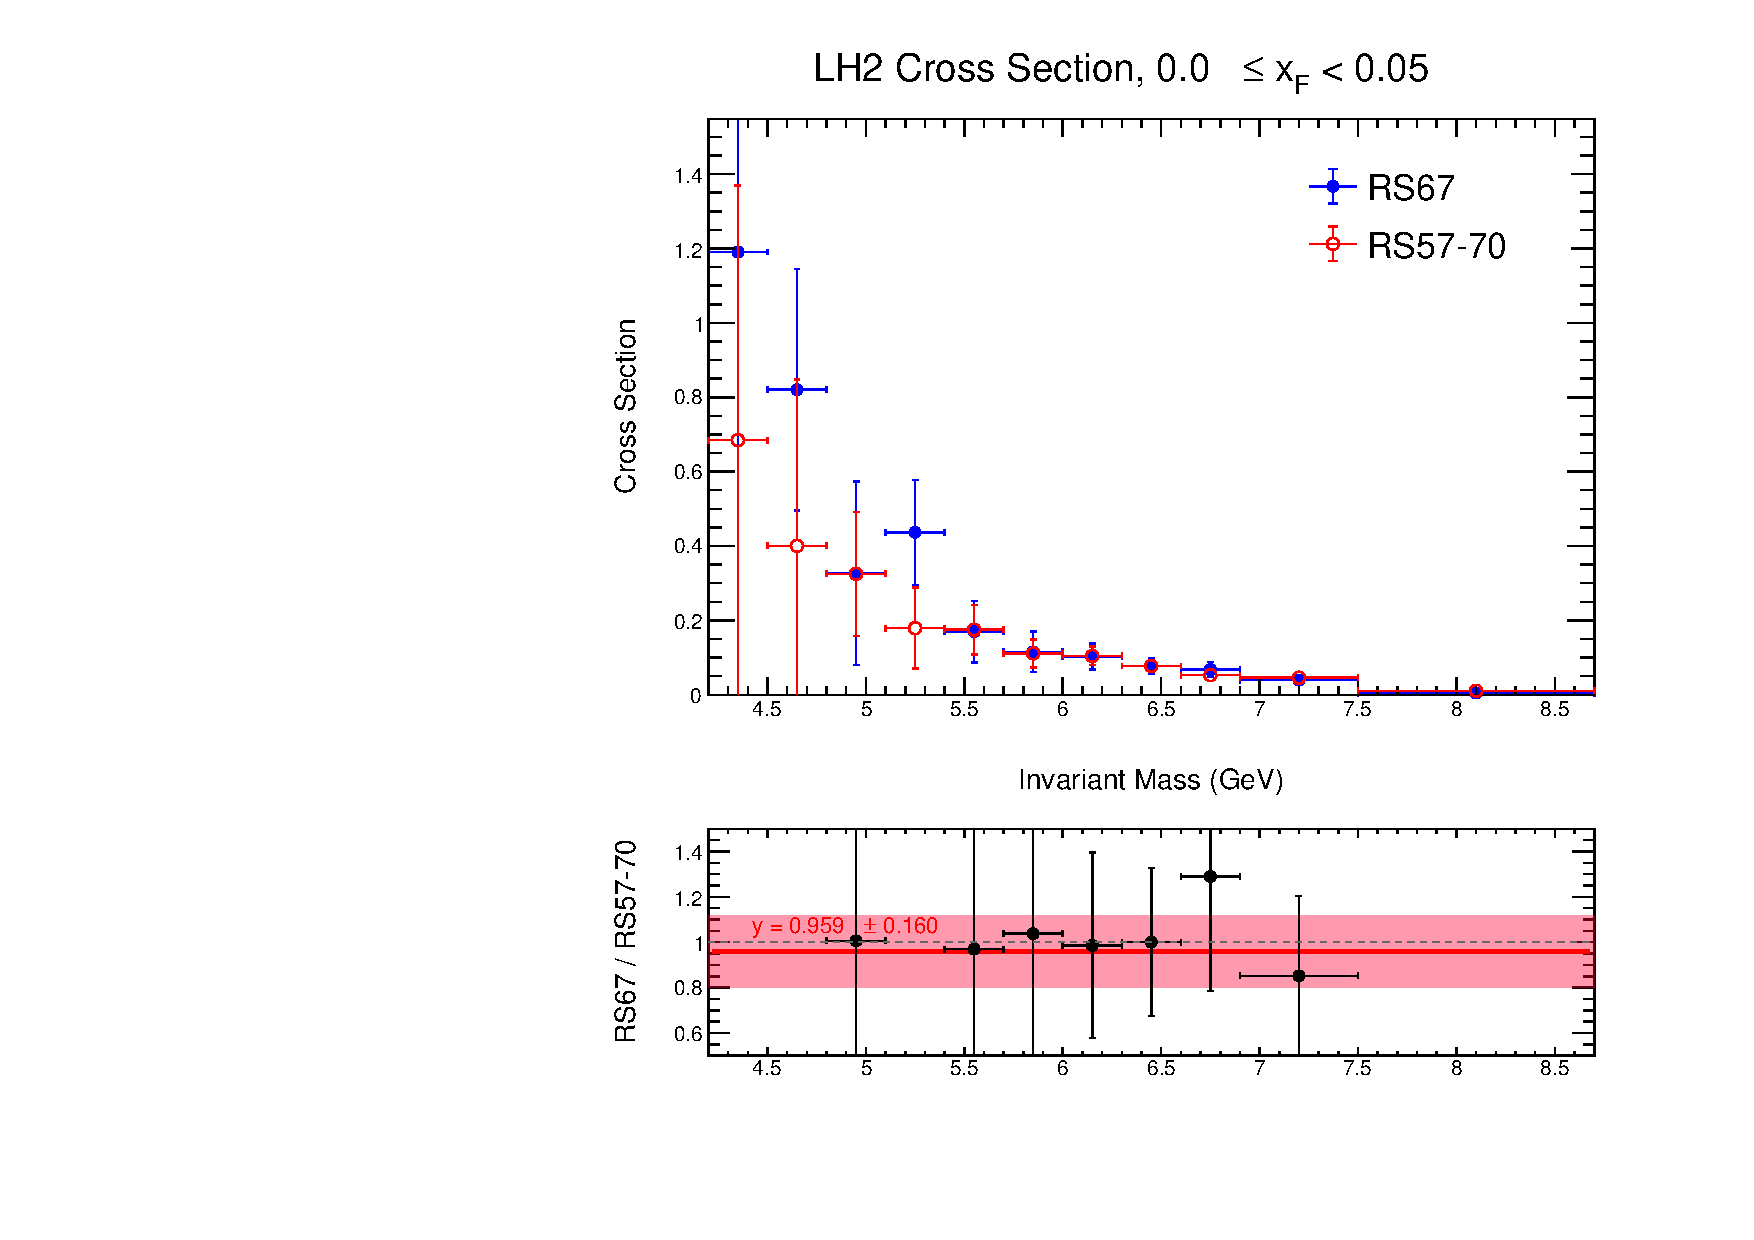
\includegraphics[width=\textwidth]{comparison_plots/XSec_Compare_LH2_xF_0.pdf}
    \end{column}
    \begin{column}{0.5\textwidth}
      \centering \textbf{Target: LD2}
      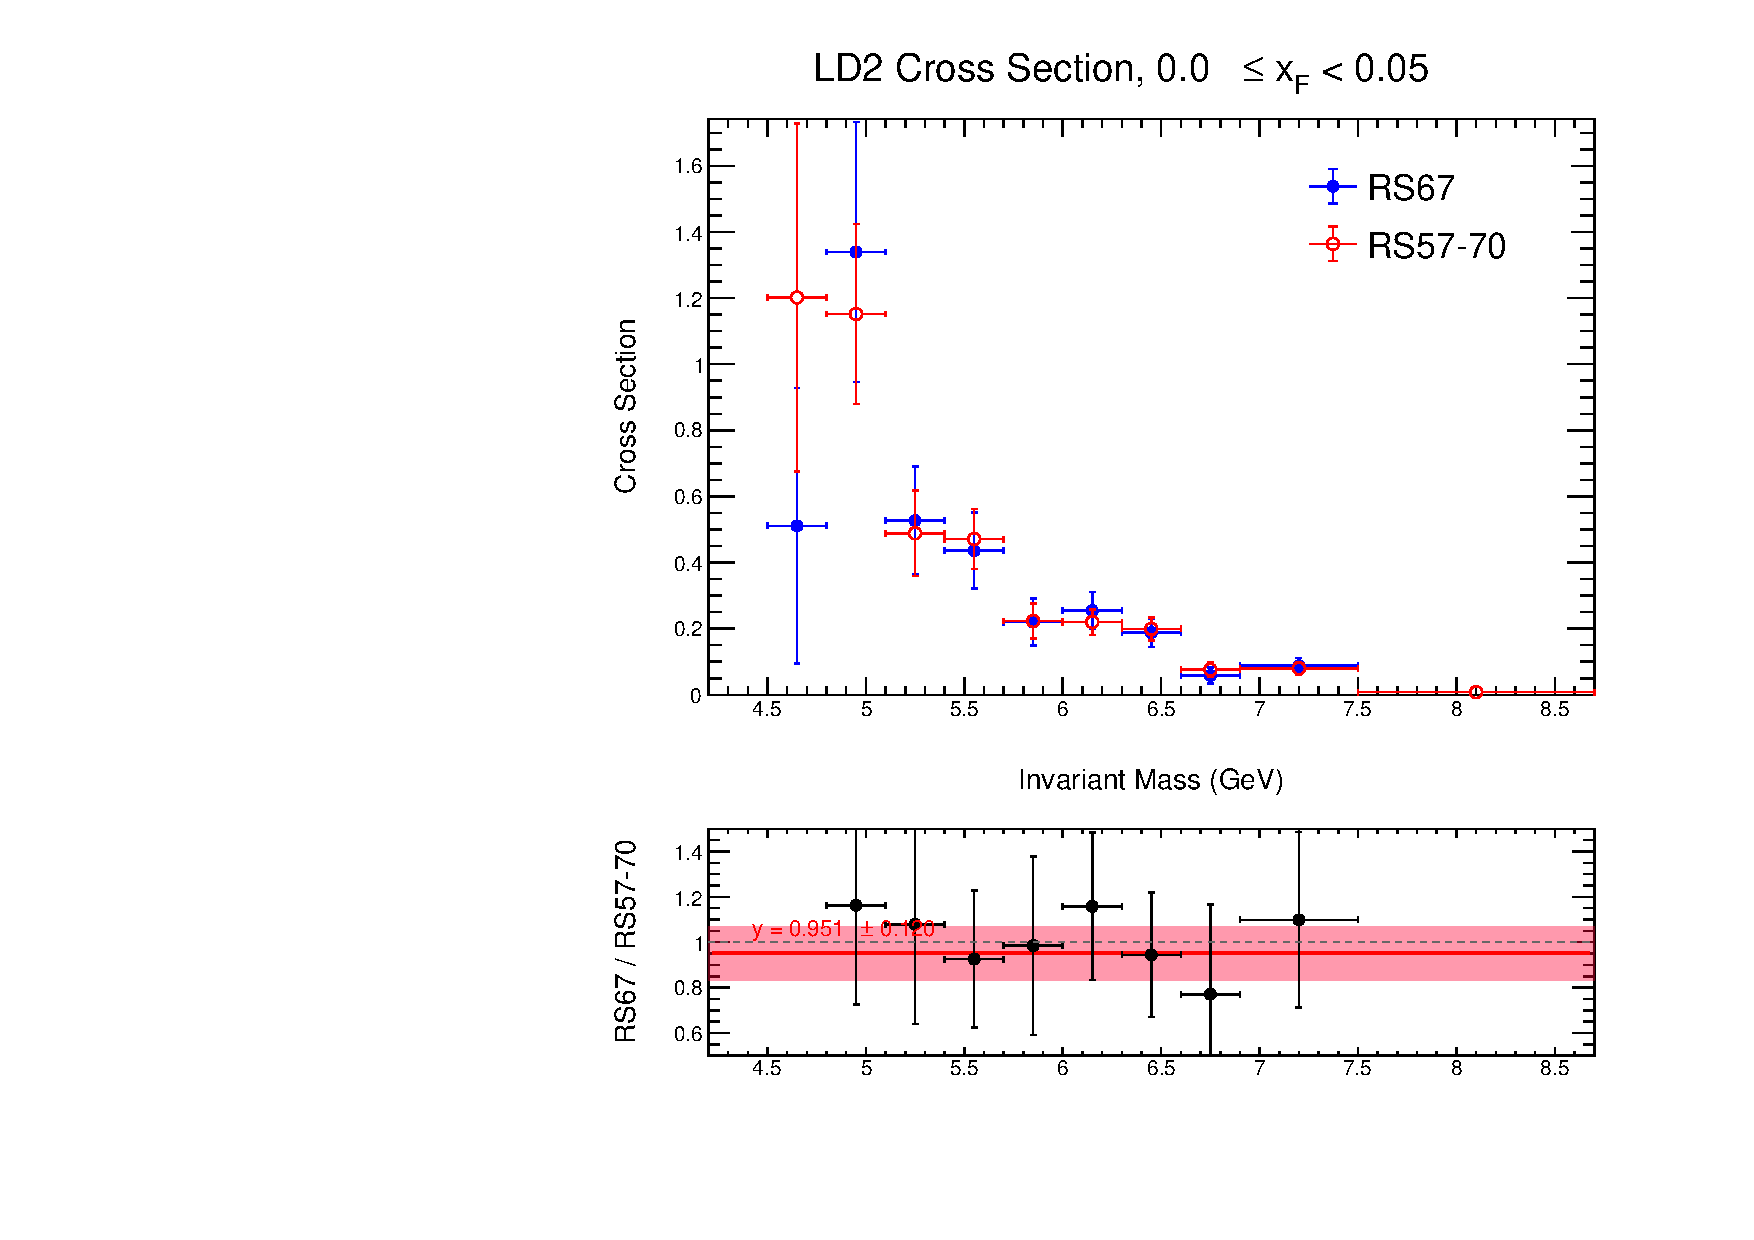
\includegraphics[width=\textwidth]{comparison_plots/XSec_Compare_LD2_xF_0.pdf}
    \end{column}
  \end{columns}
\end{frame}
\begin{frame}{Comparison for $0.05 \leq x_F < 0.1$}
  \begin{columns}
    \begin{column}{0.5\textwidth}
      \centering \textbf{Target: LH2}
      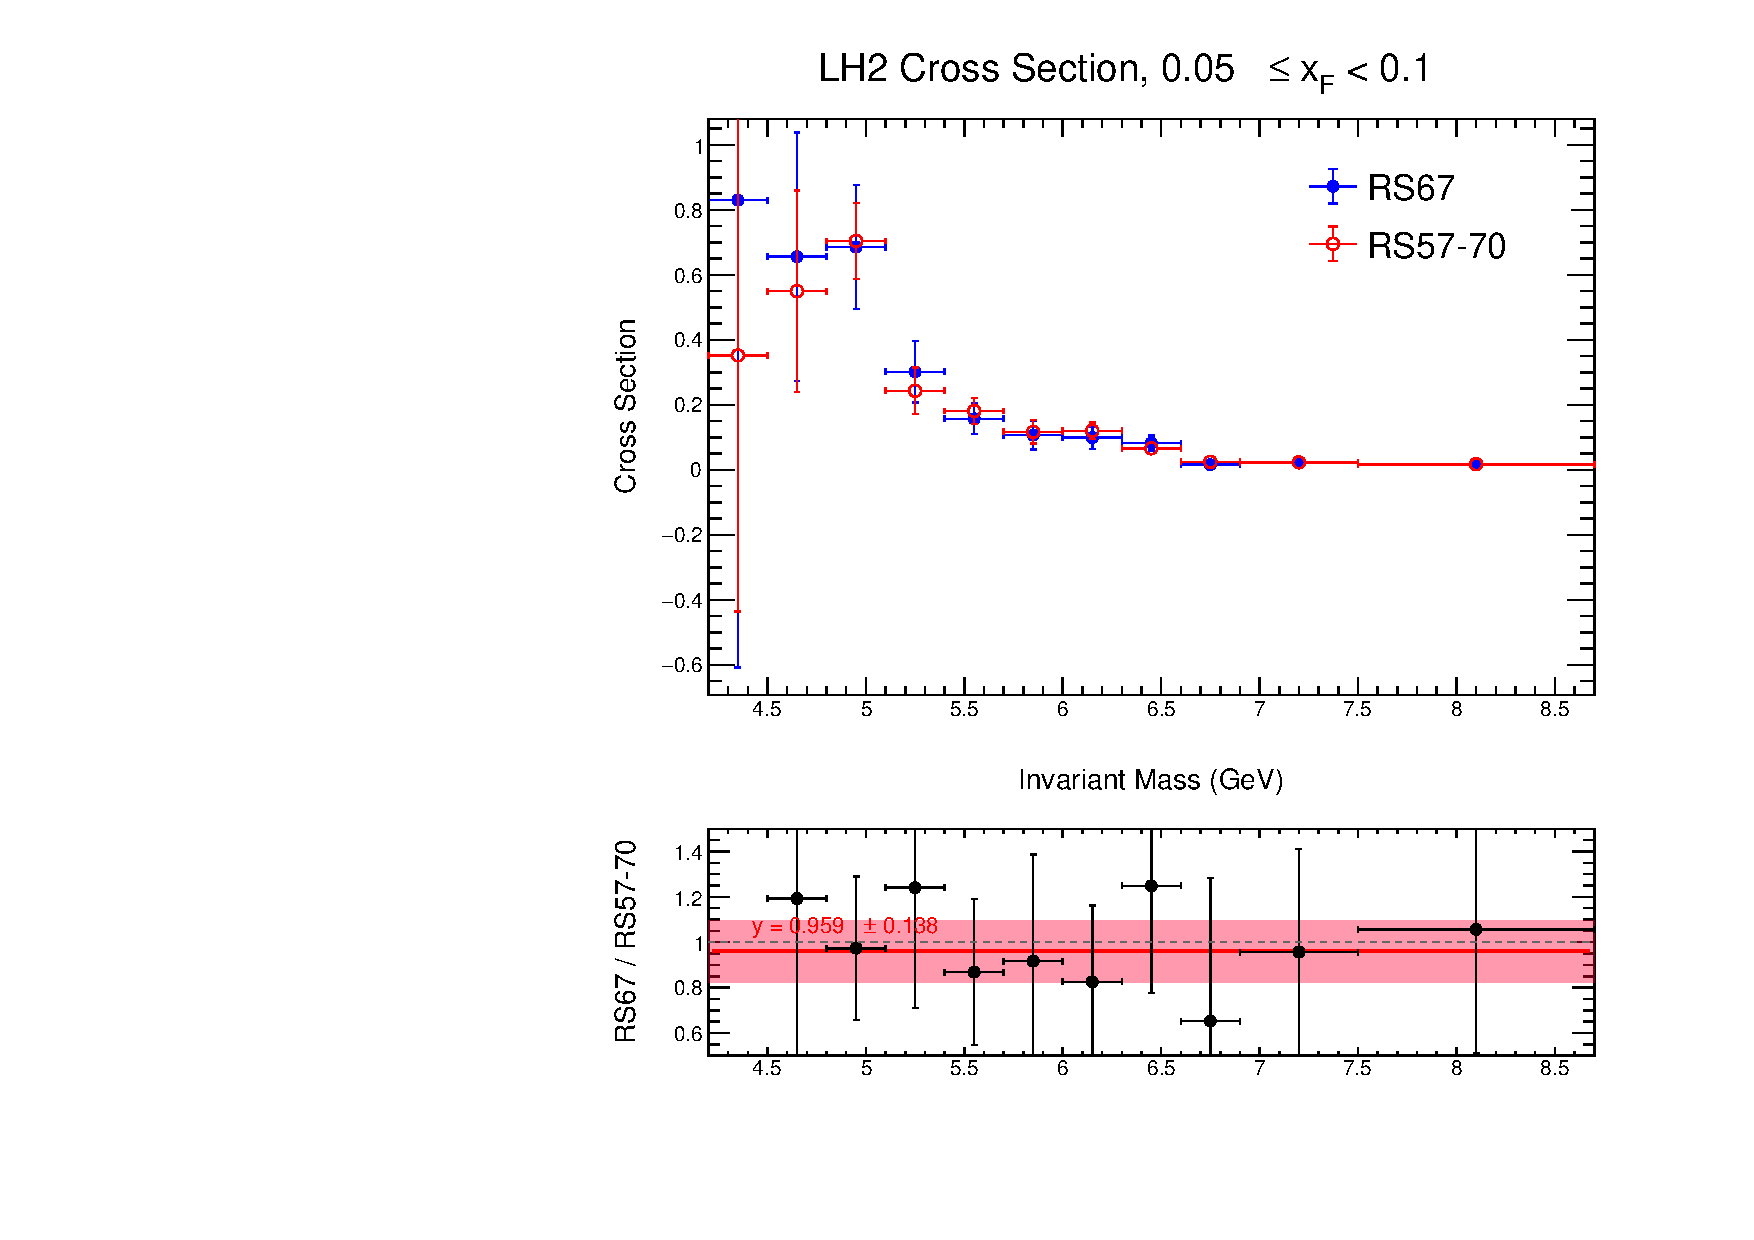
\includegraphics[width=\textwidth]{comparison_plots/XSec_Compare_LH2_xF_1.pdf}
    \end{column}
    \begin{column}{0.5\textwidth}
      \centering \textbf{Target: LD2}
      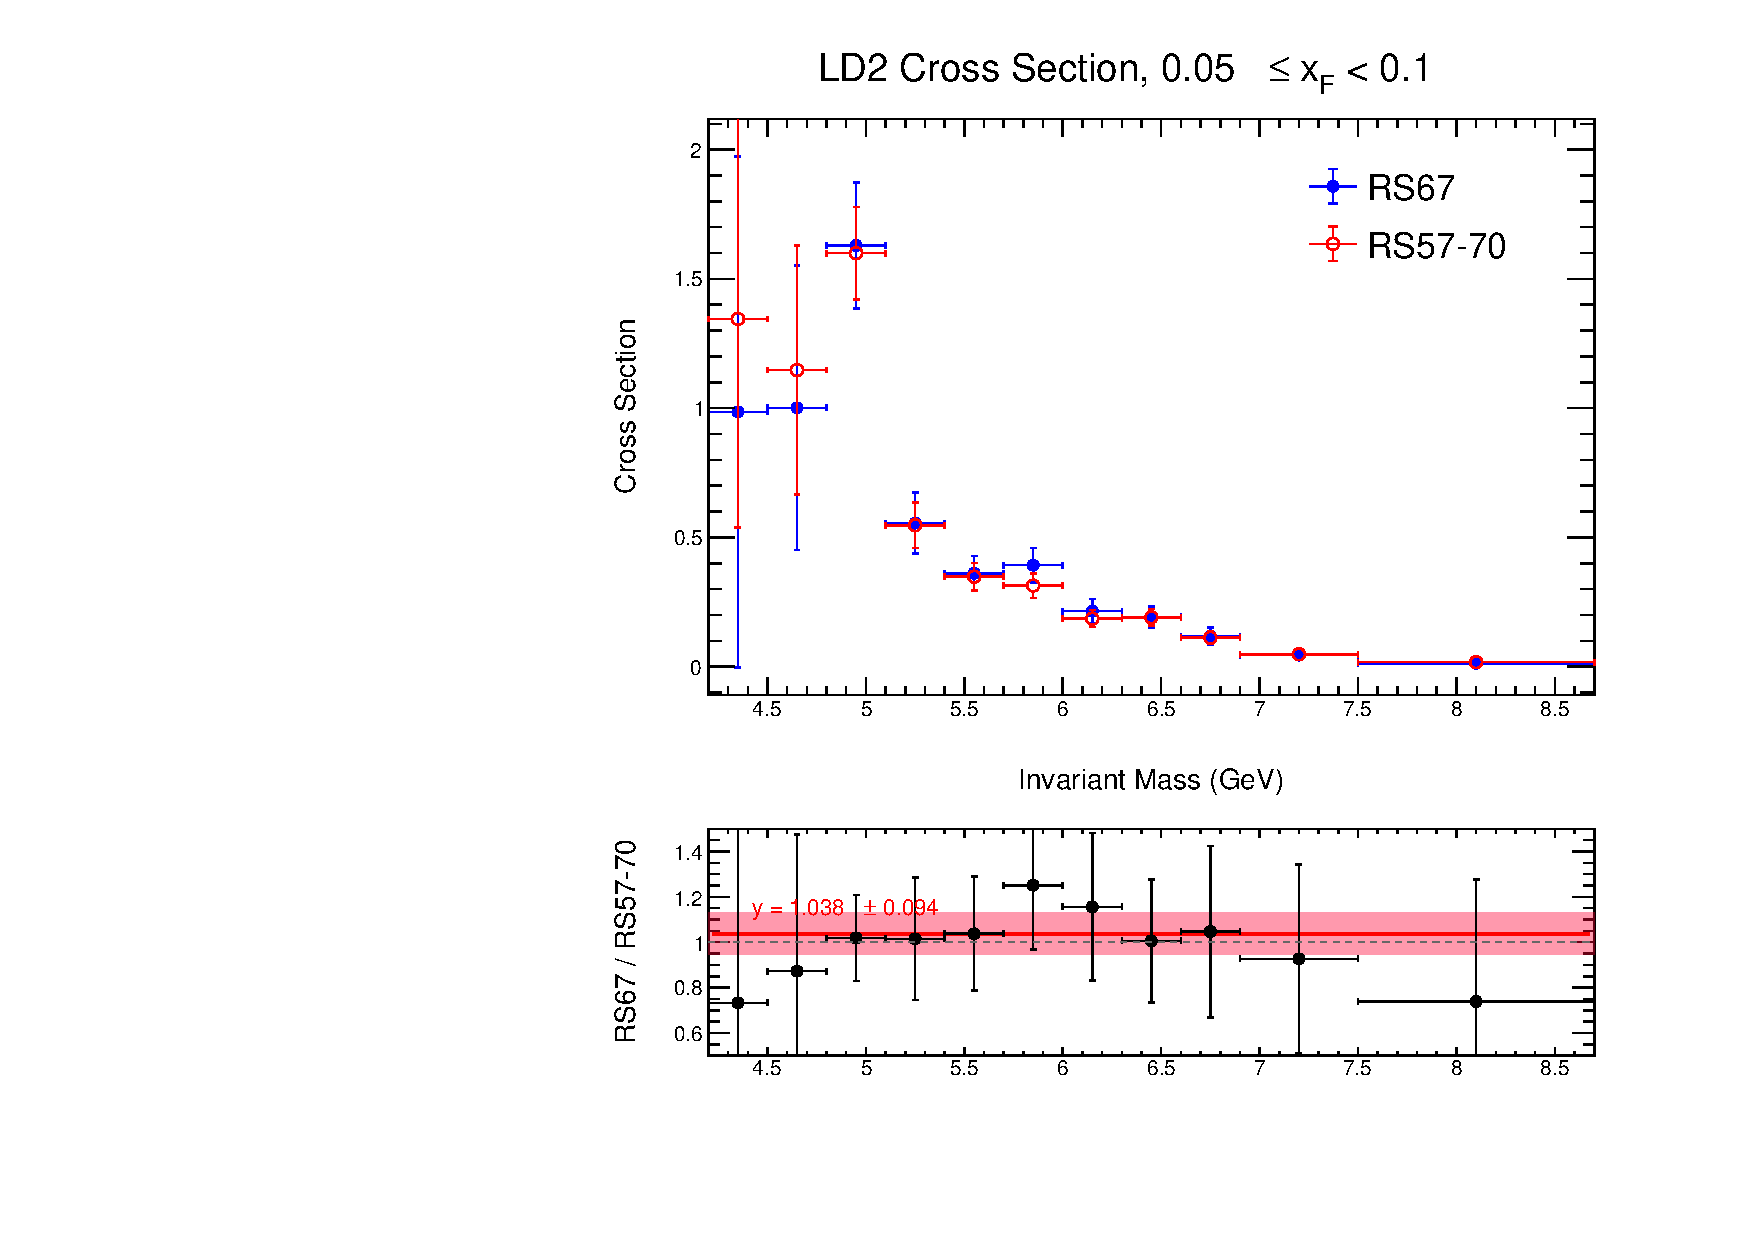
\includegraphics[width=\textwidth]{comparison_plots/XSec_Compare_LD2_xF_1.pdf}
    \end{column}
  \end{columns}
\end{frame}
\begin{frame}{Comparison for $0.1 \leq x_F < 0.15$}
  \begin{columns}
    \begin{column}{0.5\textwidth}
      \centering \textbf{Target: LH2}
      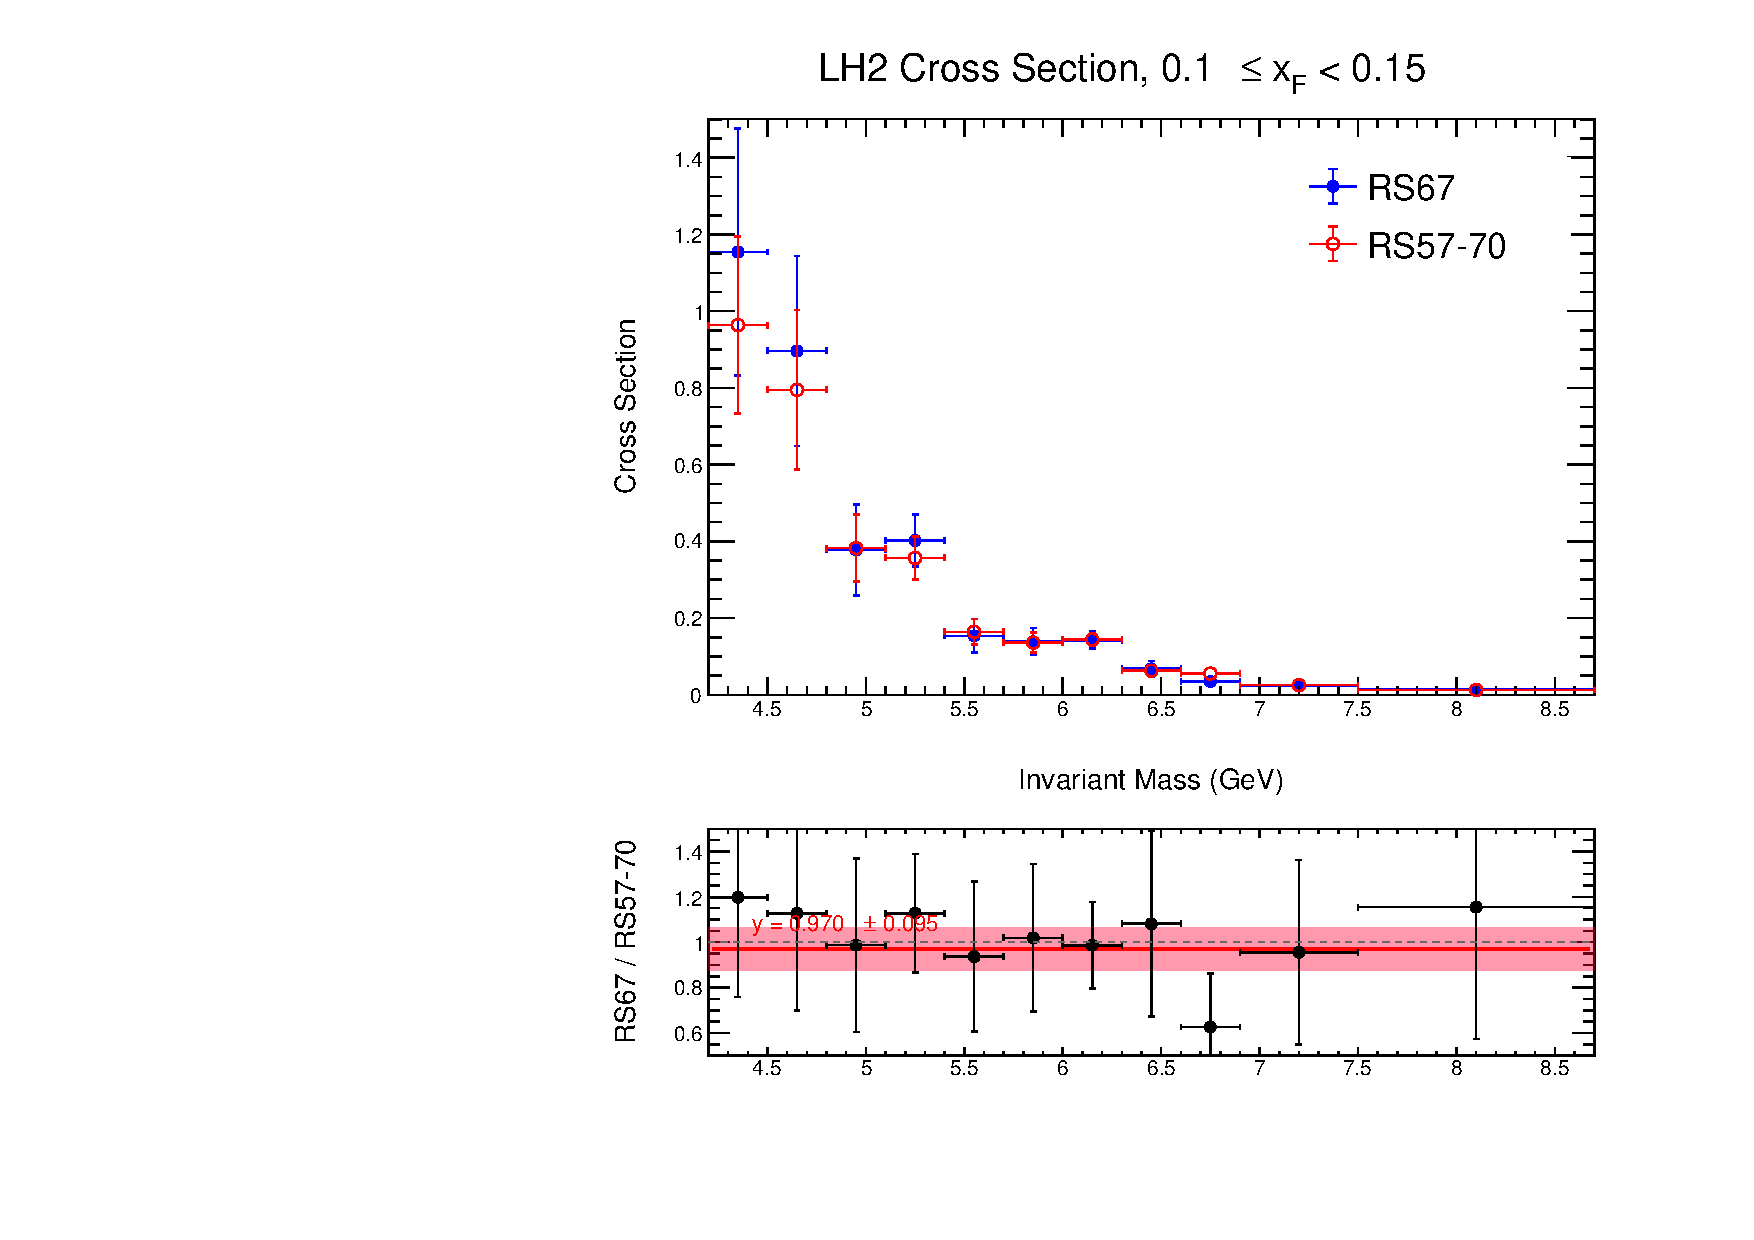
\includegraphics[width=\textwidth]{comparison_plots/XSec_Compare_LH2_xF_2.pdf}
    \end{column}
    \begin{column}{0.5\textwidth}
      \centering \textbf{Target: LD2}
      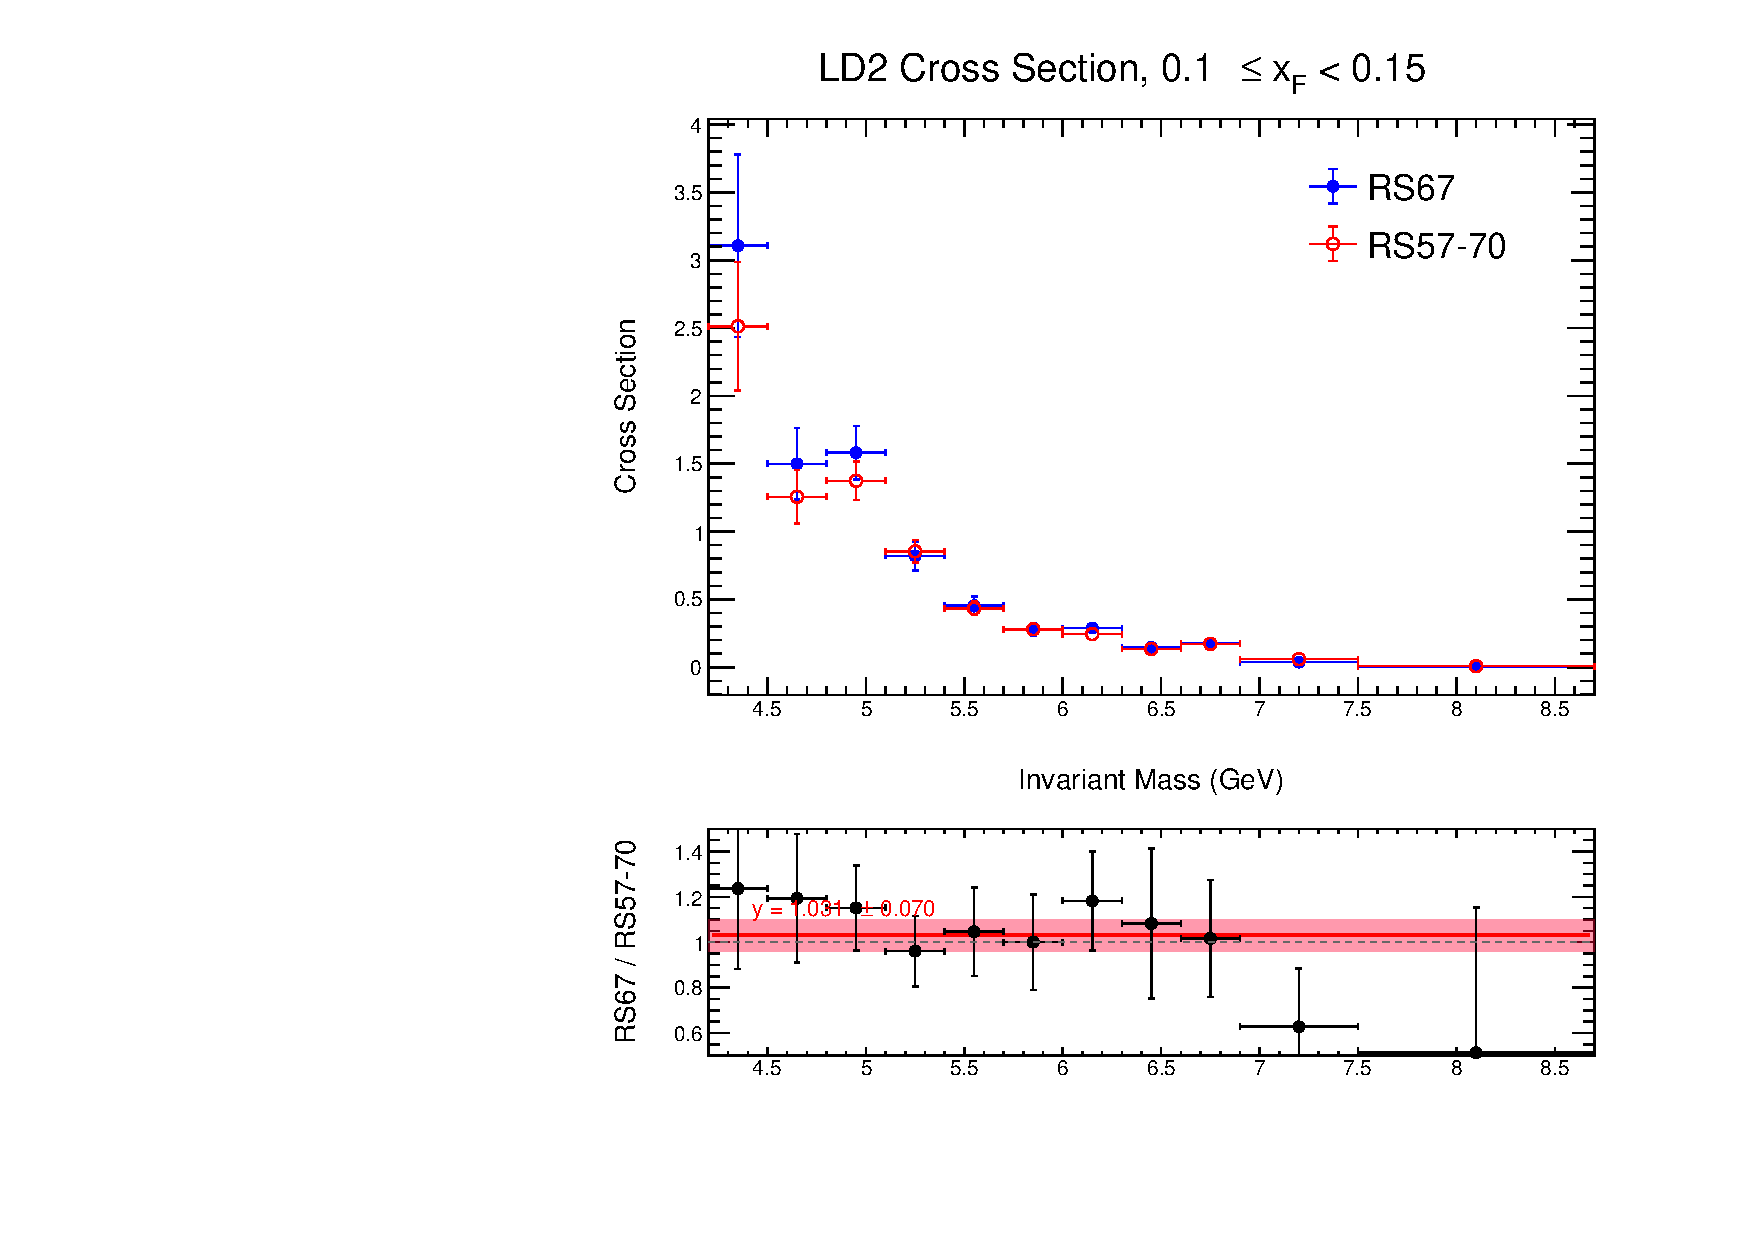
\includegraphics[width=\textwidth]{comparison_plots/XSec_Compare_LD2_xF_2.pdf}
    \end{column}
  \end{columns}
\end{frame}
\begin{frame}{Comparison for $0.15 \leq x_F < 0.2$}
  \begin{columns}
    \begin{column}{0.5\textwidth}
      \centering \textbf{Target: LH2}
      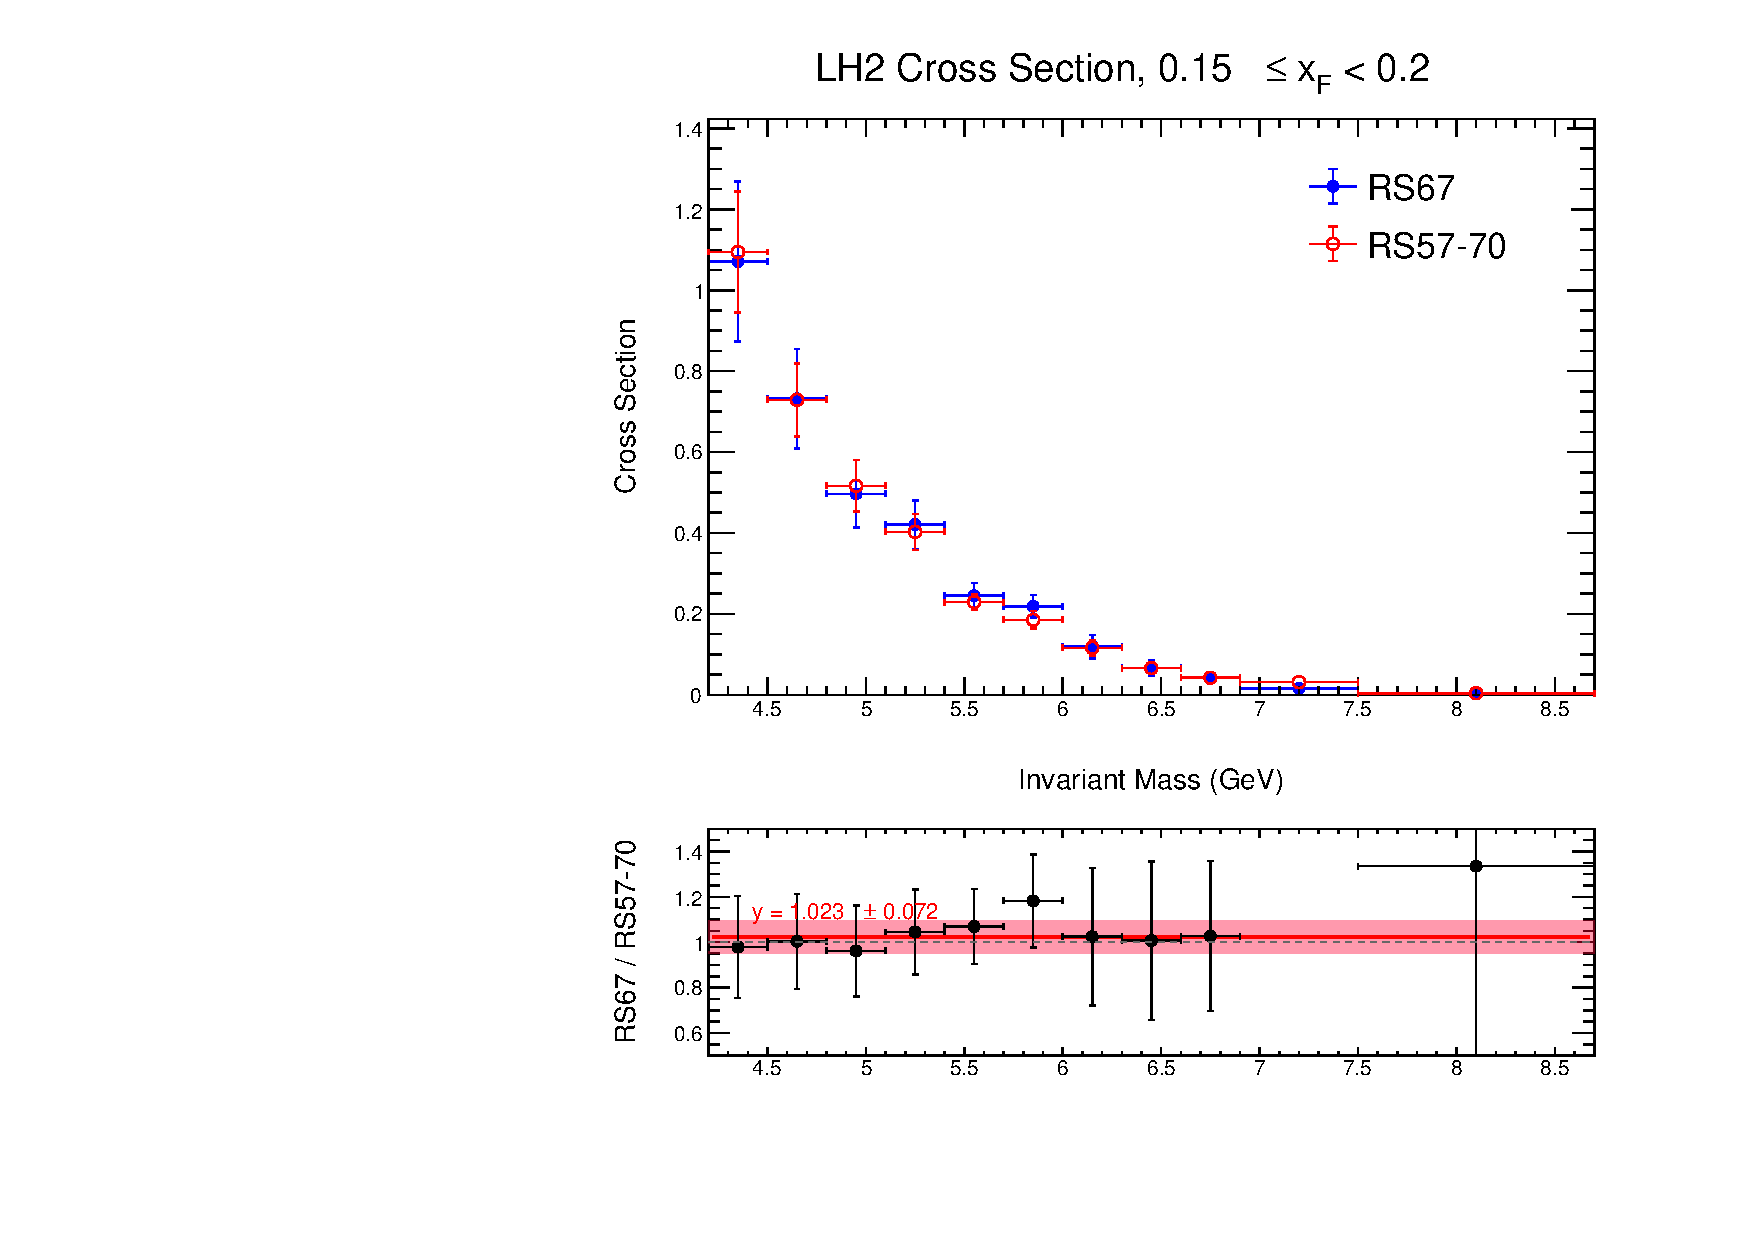
\includegraphics[width=\textwidth]{comparison_plots/XSec_Compare_LH2_xF_3.pdf}
    \end{column}
    \begin{column}{0.5\textwidth}
      \centering \textbf{Target: LD2}
      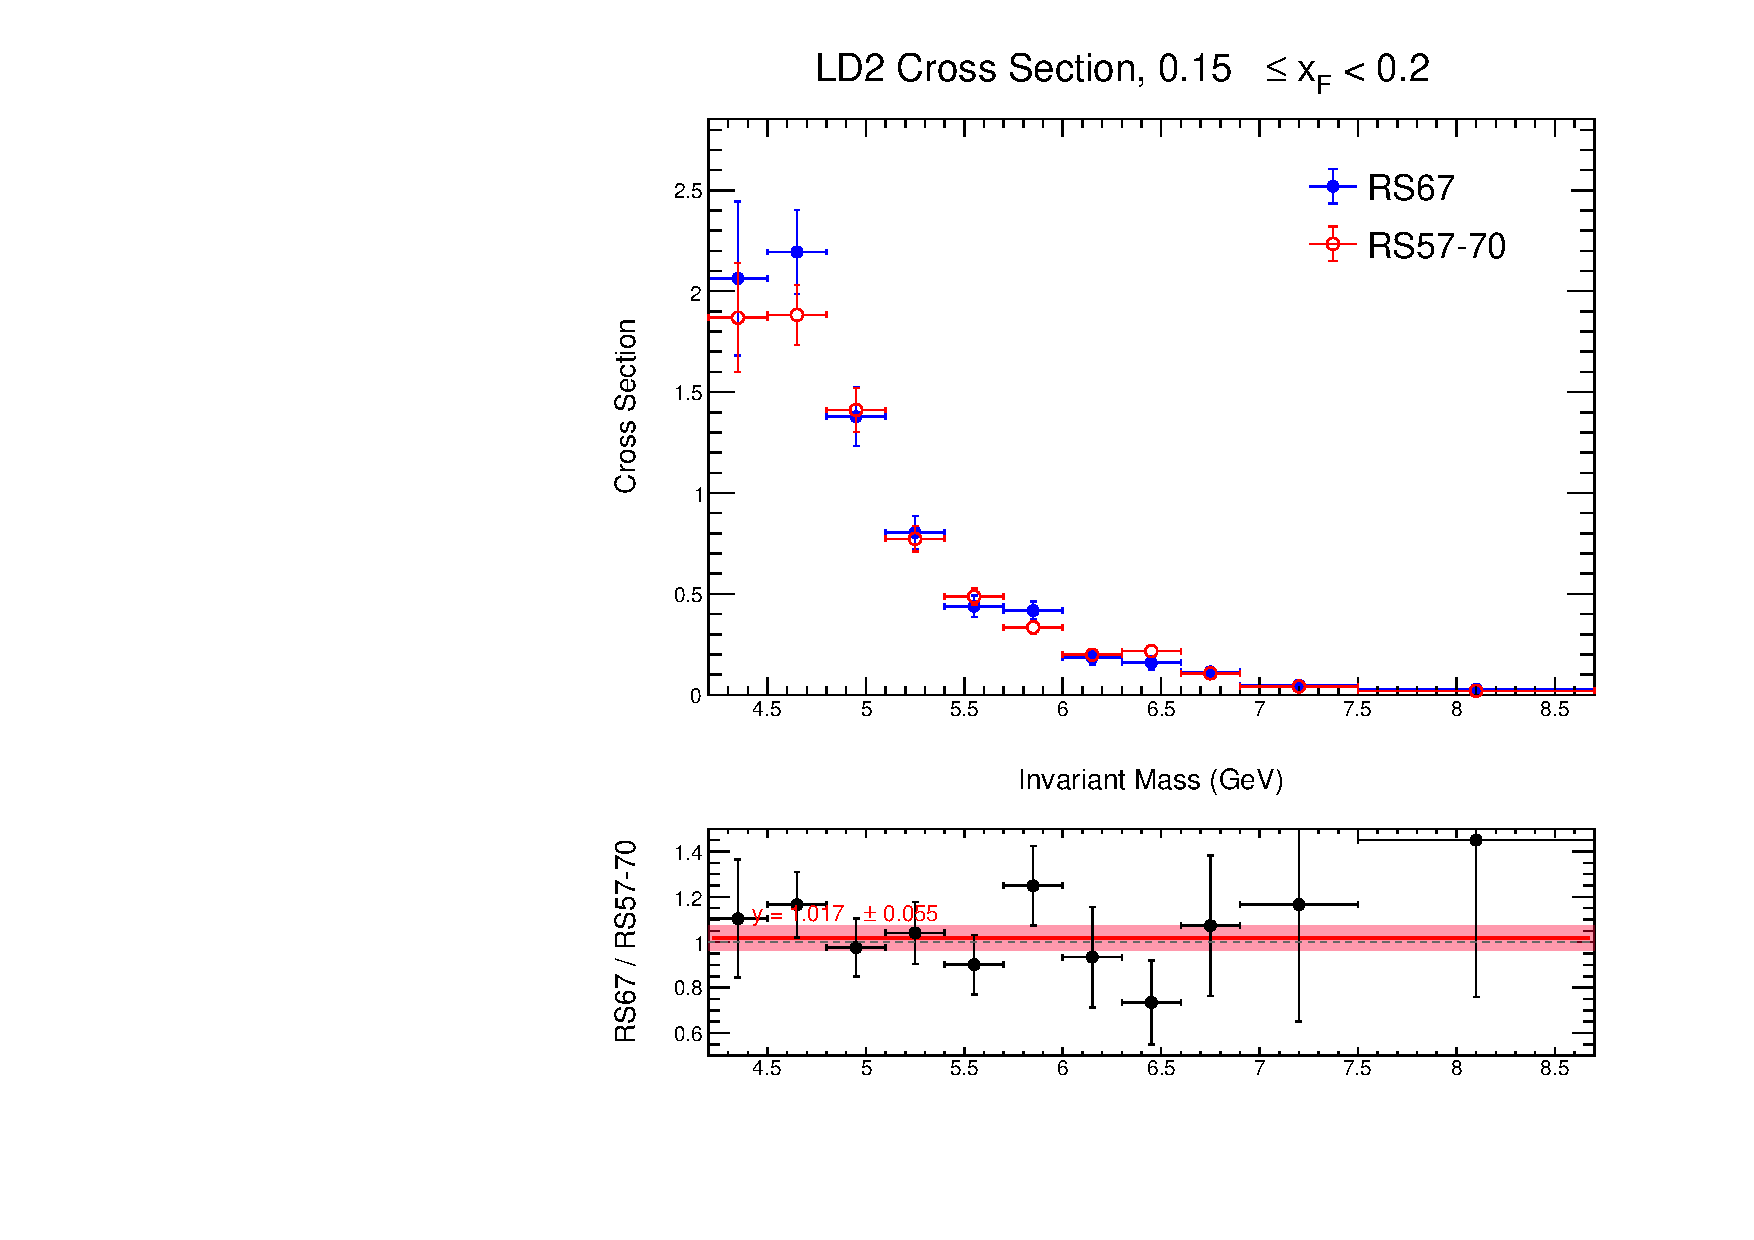
\includegraphics[width=\textwidth]{comparison_plots/XSec_Compare_LD2_xF_3.pdf}
    \end{column}
  \end{columns}
\end{frame}
\begin{frame}{Comparison for $0.2 \leq x_F < 0.25$}
  \begin{columns}
    \begin{column}{0.5\textwidth}
      \centering \textbf{Target: LH2}
      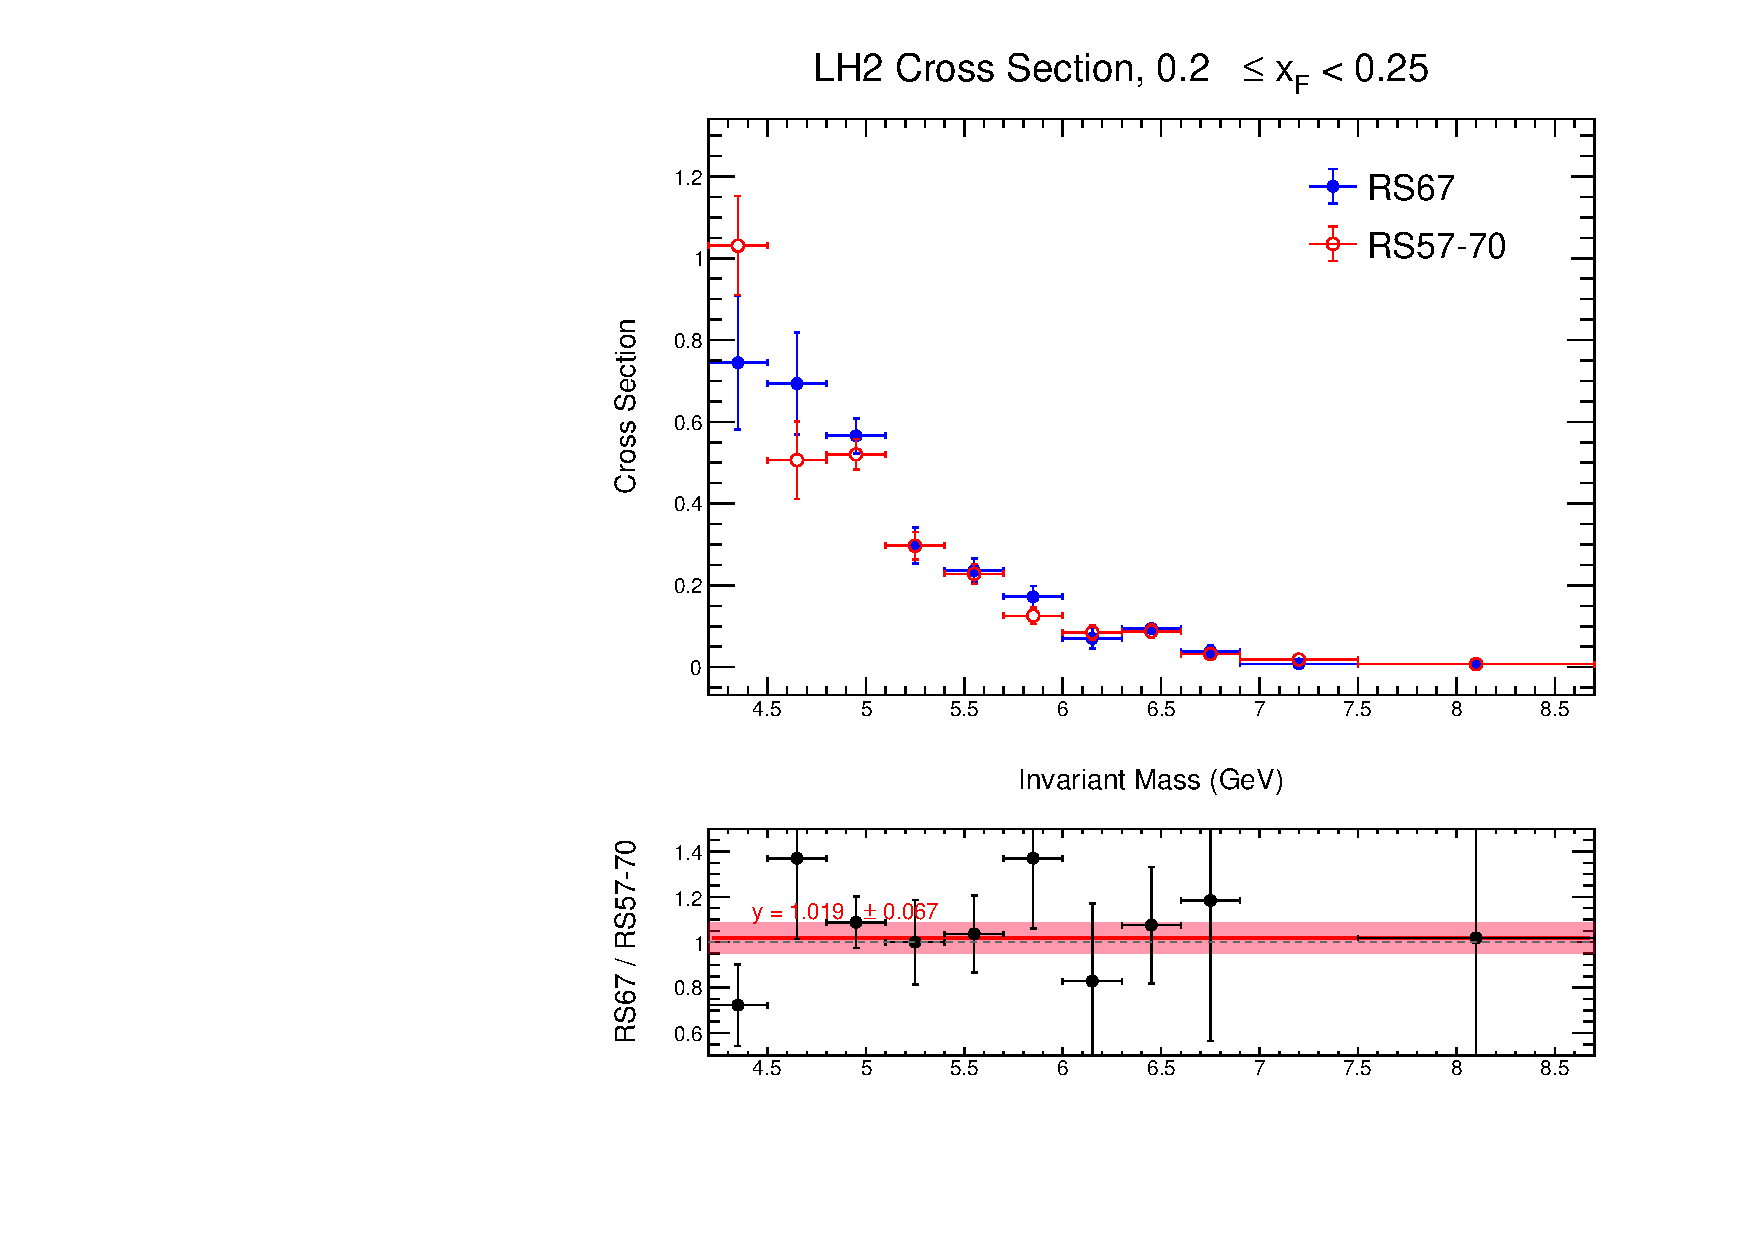
\includegraphics[width=\textwidth]{comparison_plots/XSec_Compare_LH2_xF_4.pdf}
    \end{column}
    \begin{column}{0.5\textwidth}
      \centering \textbf{Target: LD2}
      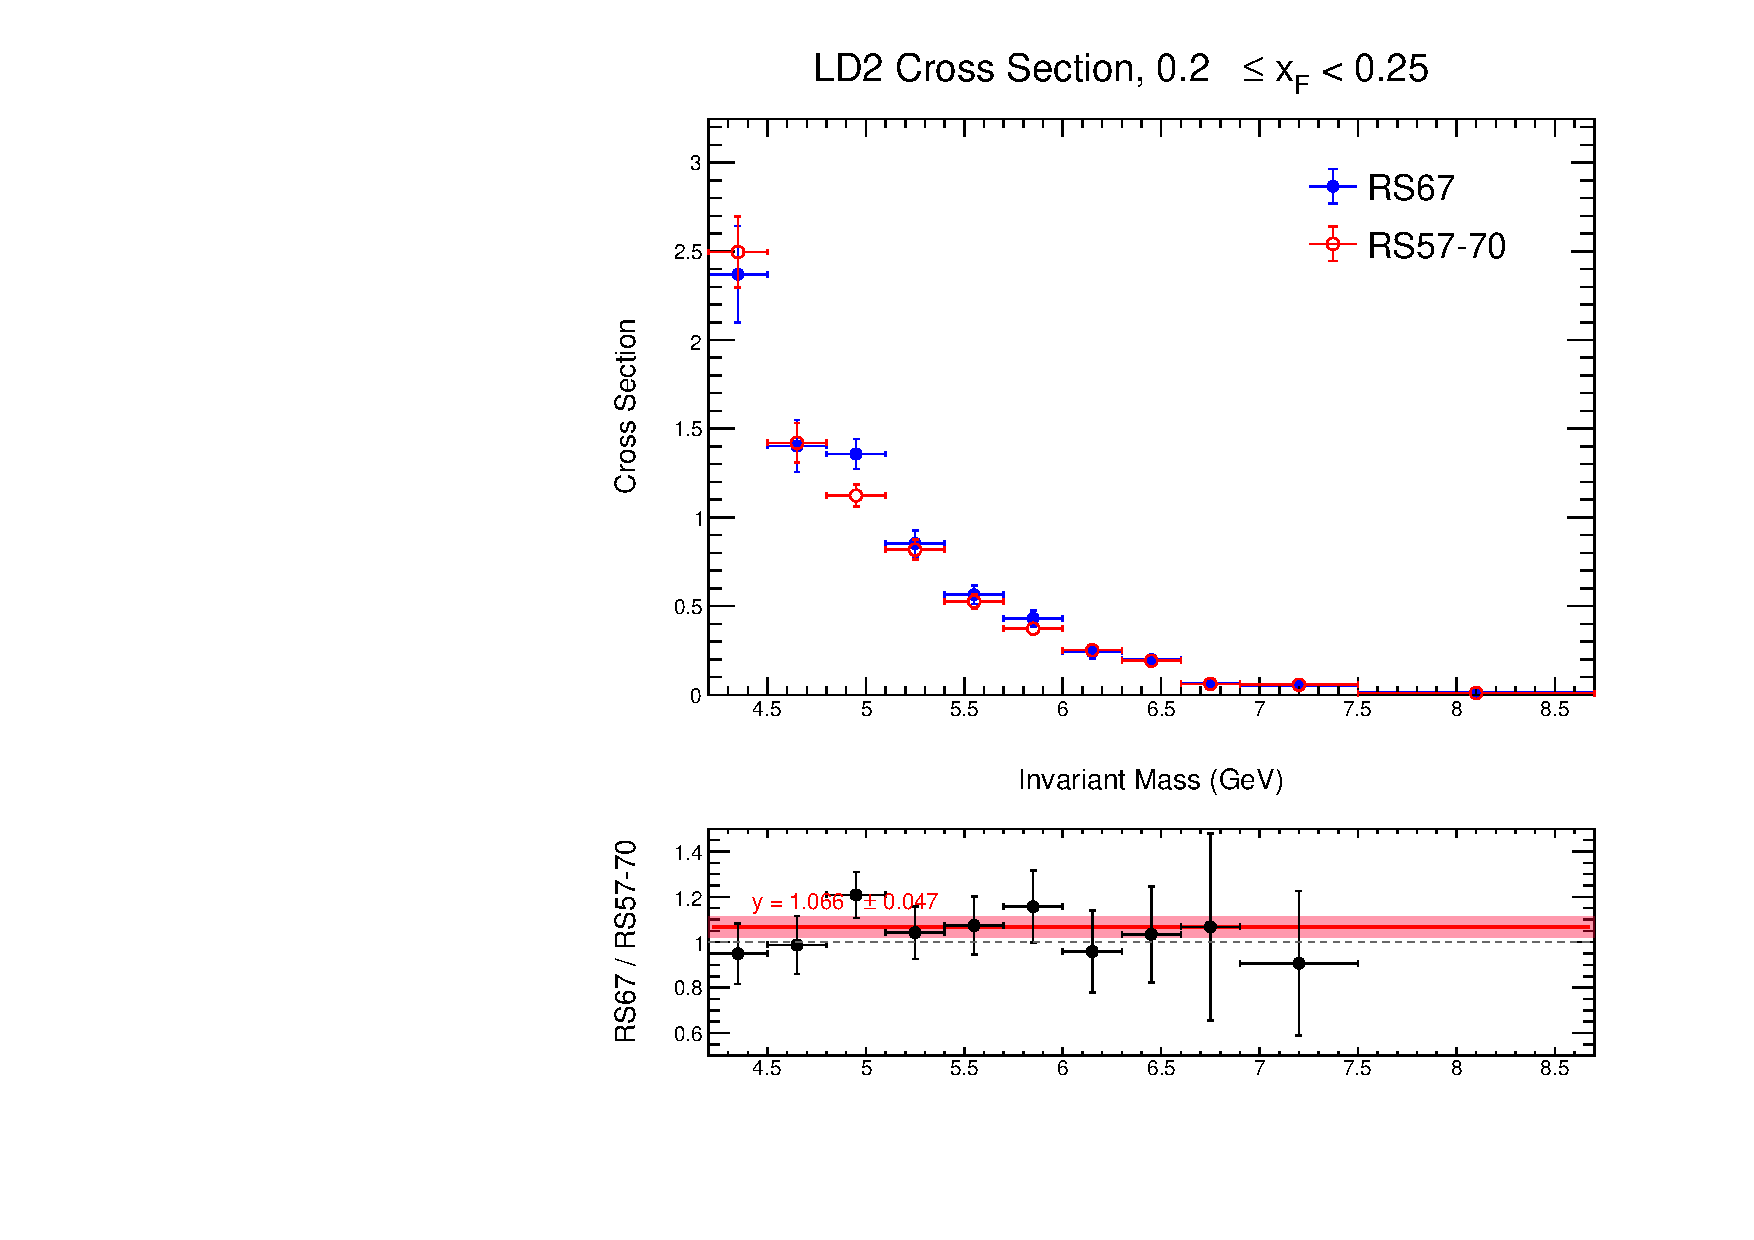
\includegraphics[width=\textwidth]{comparison_plots/XSec_Compare_LD2_xF_4.pdf}
    \end{column}
  \end{columns}
\end{frame}
\begin{frame}{Comparison for $0.25 \leq x_F < 0.3$}
  \begin{columns}
    \begin{column}{0.5\textwidth}
      \centering \textbf{Target: LH2}
      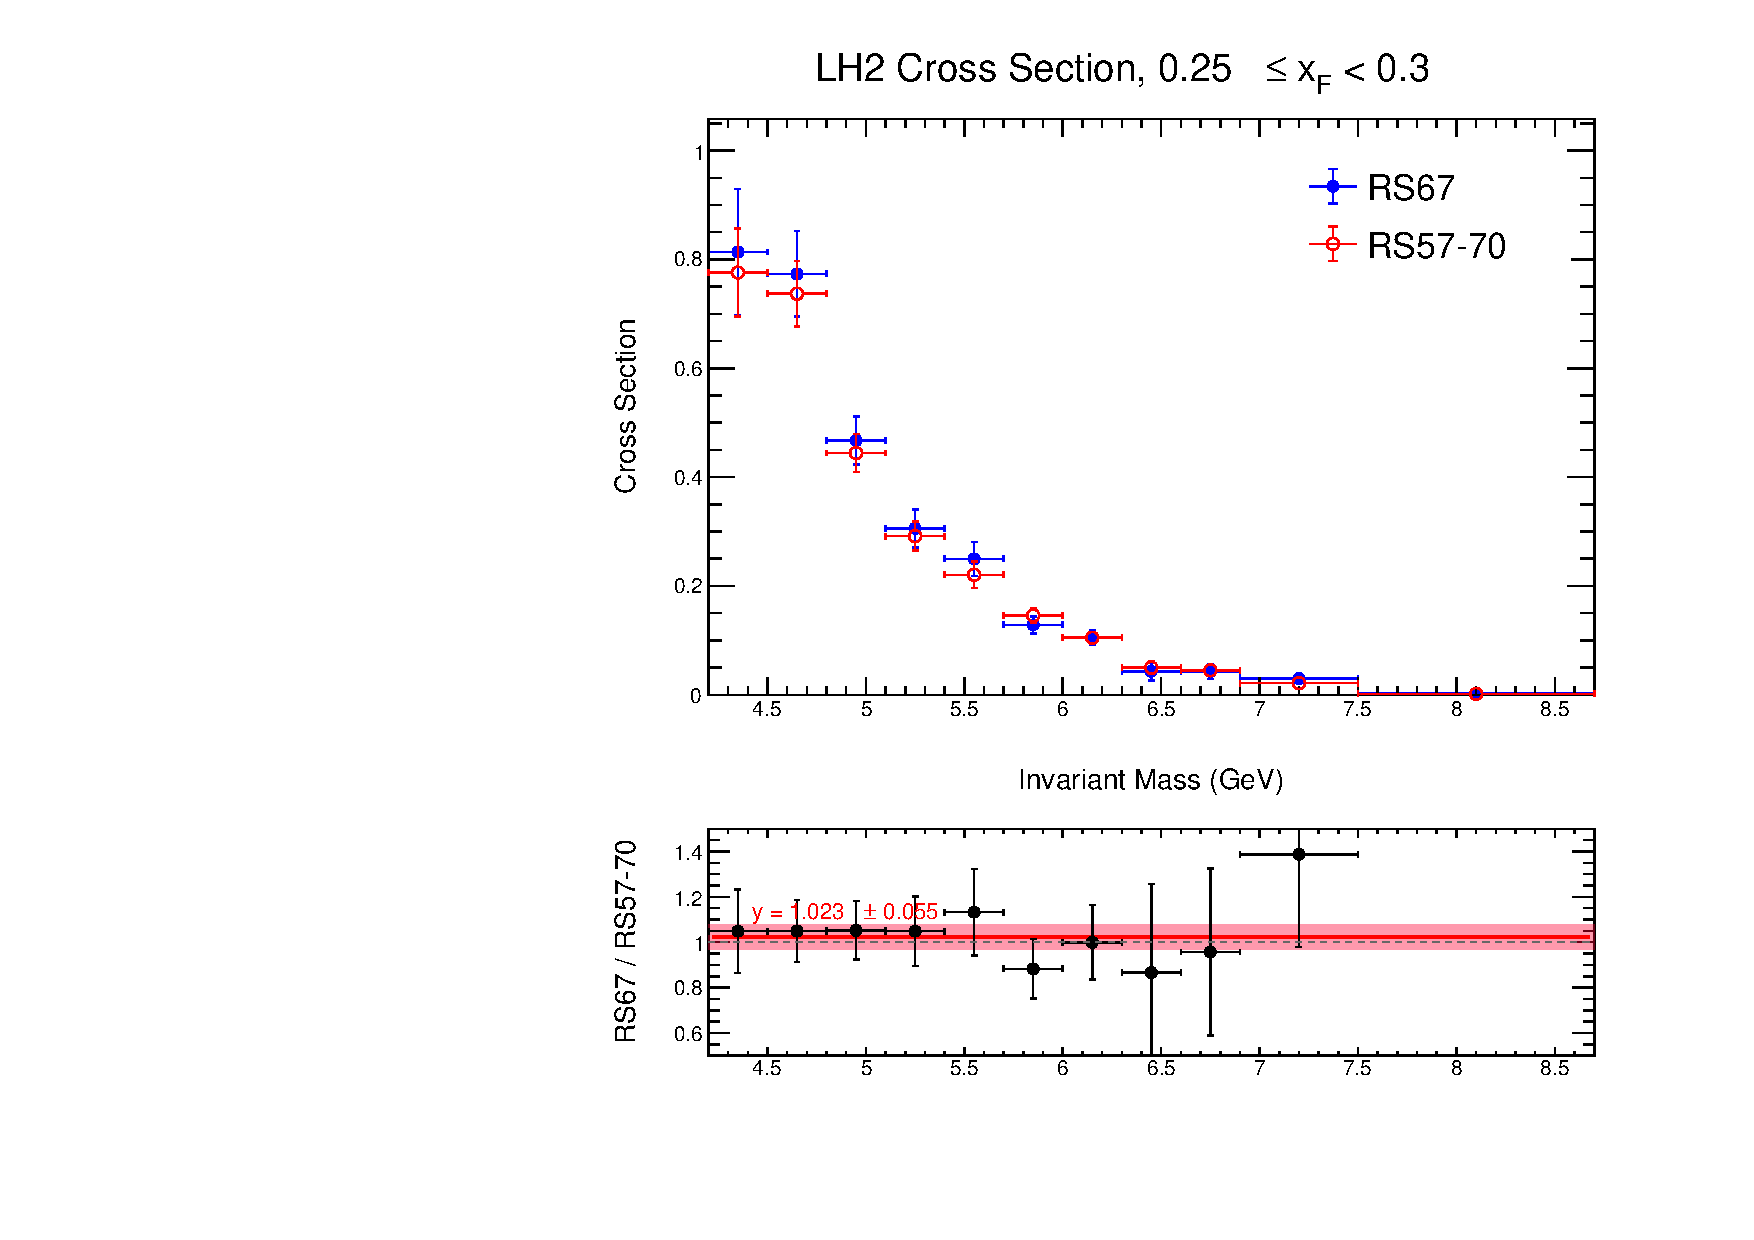
\includegraphics[width=\textwidth]{comparison_plots/XSec_Compare_LH2_xF_5.pdf}
    \end{column}
    \begin{column}{0.5\textwidth}
      \centering \textbf{Target: LD2}
      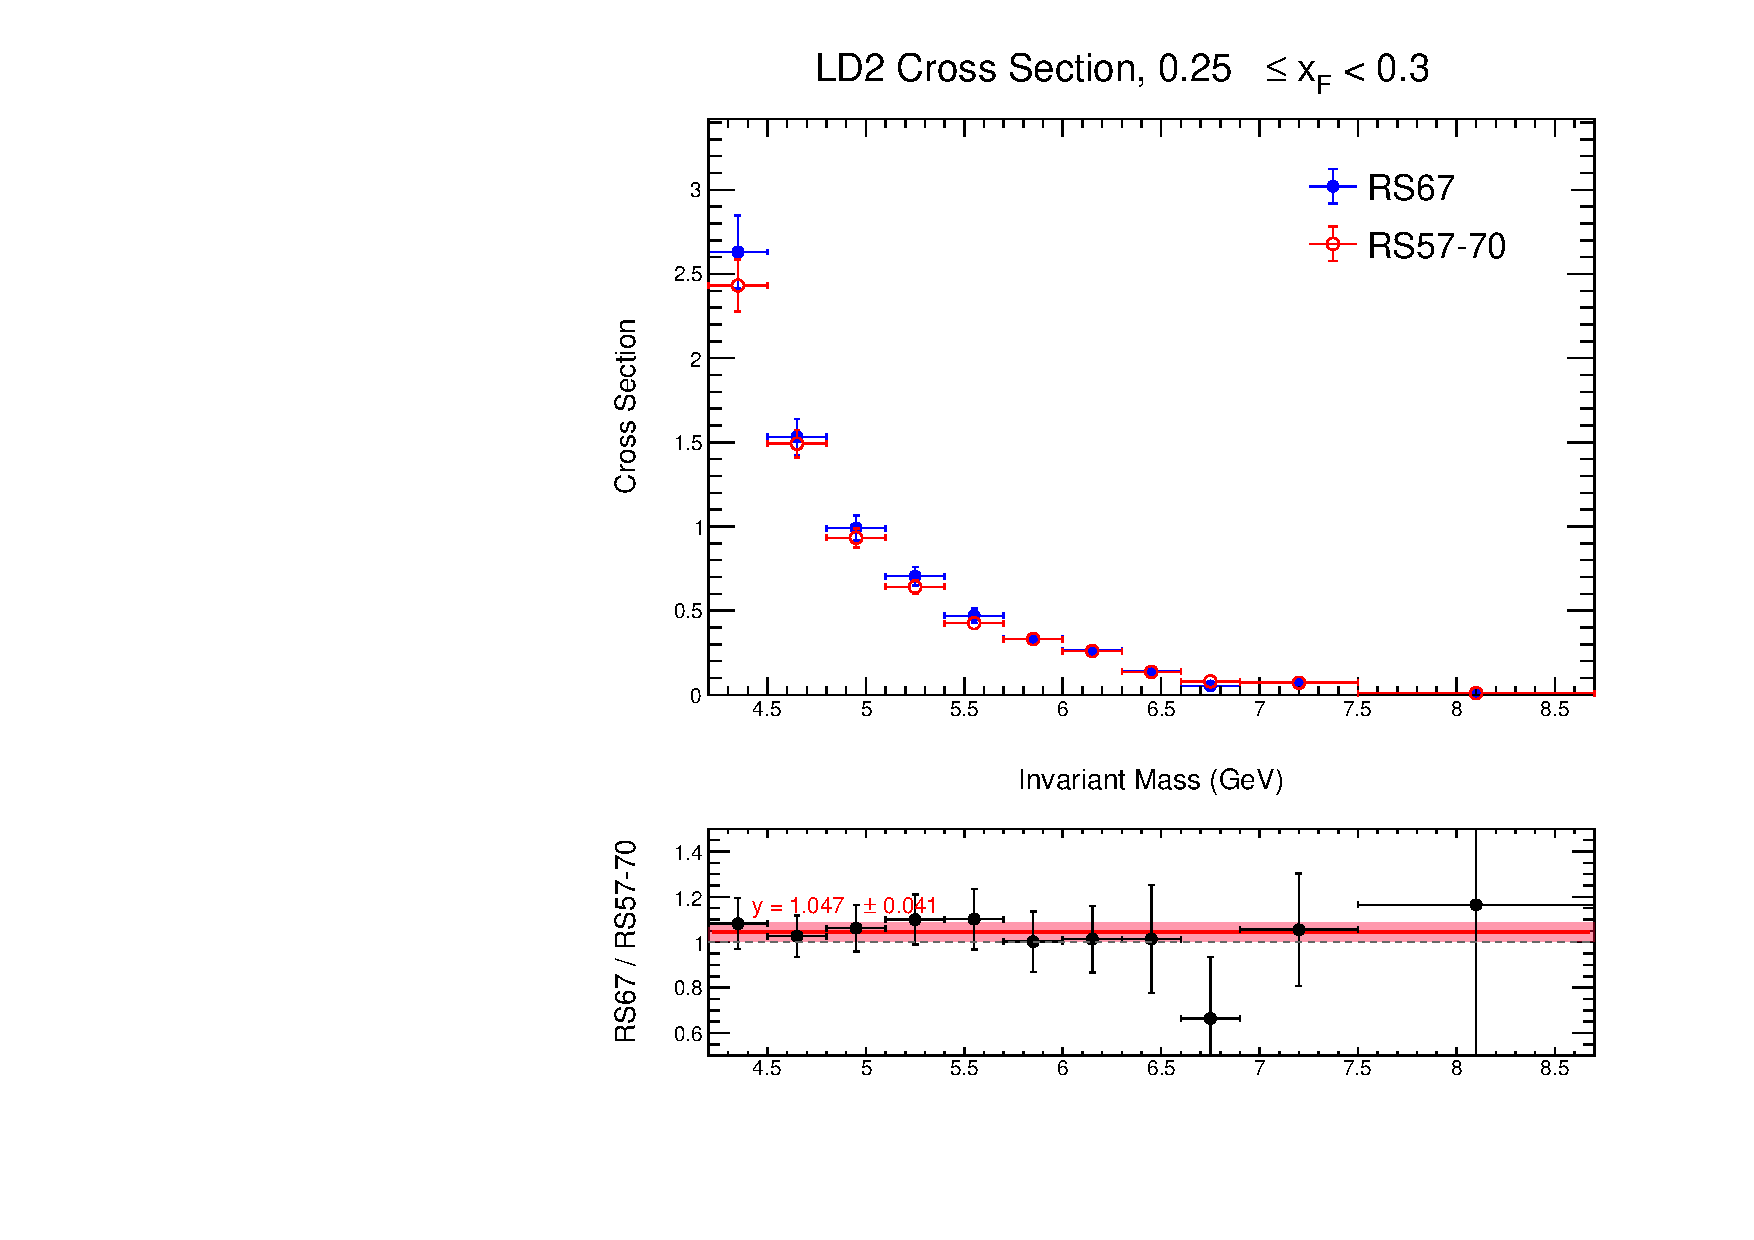
\includegraphics[width=\textwidth]{comparison_plots/XSec_Compare_LD2_xF_5.pdf}
    \end{column}
  \end{columns}
\end{frame}
\begin{frame}{Comparison for $0.3 \leq x_F < 0.35$}
  \begin{columns}
    \begin{column}{0.5\textwidth}
      \centering \textbf{Target: LH2}
      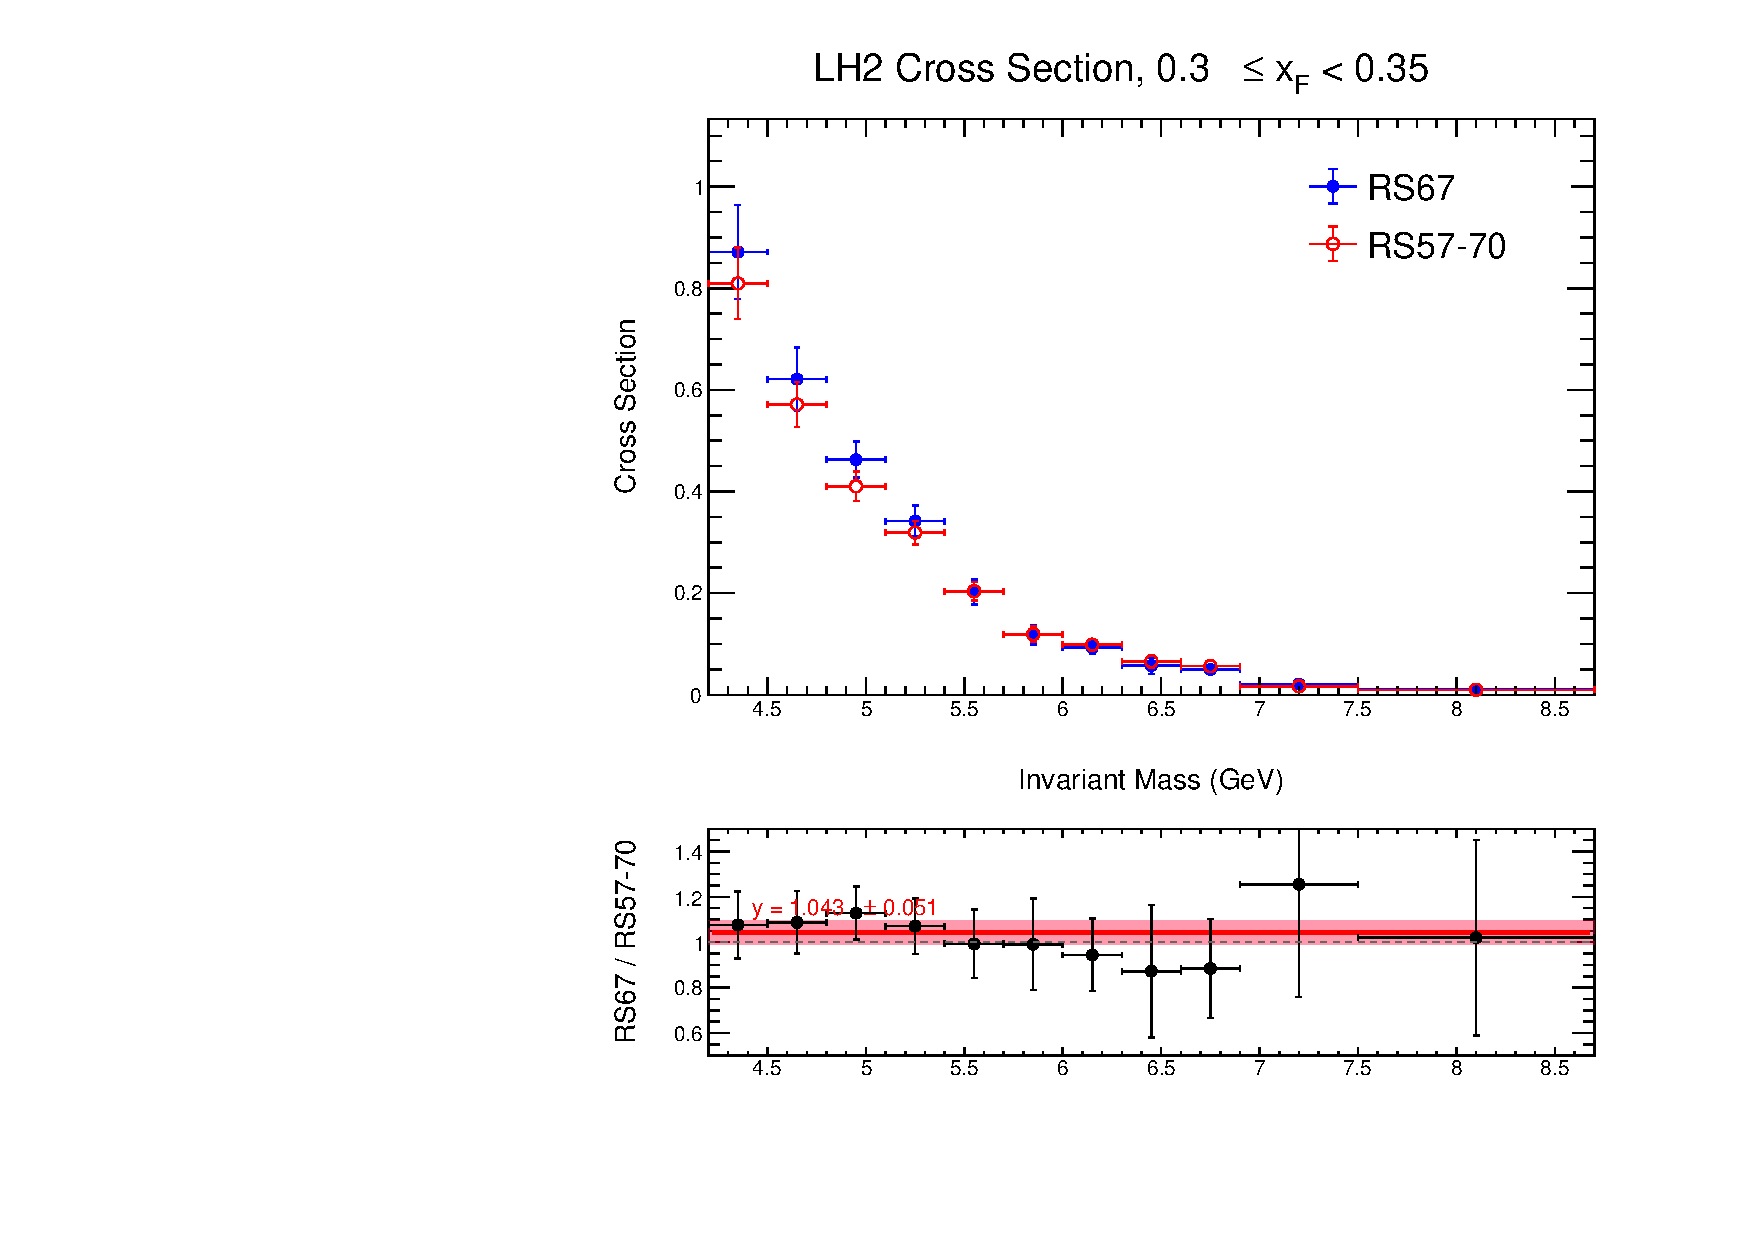
\includegraphics[width=\textwidth]{comparison_plots/XSec_Compare_LH2_xF_6.pdf}
    \end{column}
    \begin{column}{0.5\textwidth}
      \centering \textbf{Target: LD2}
      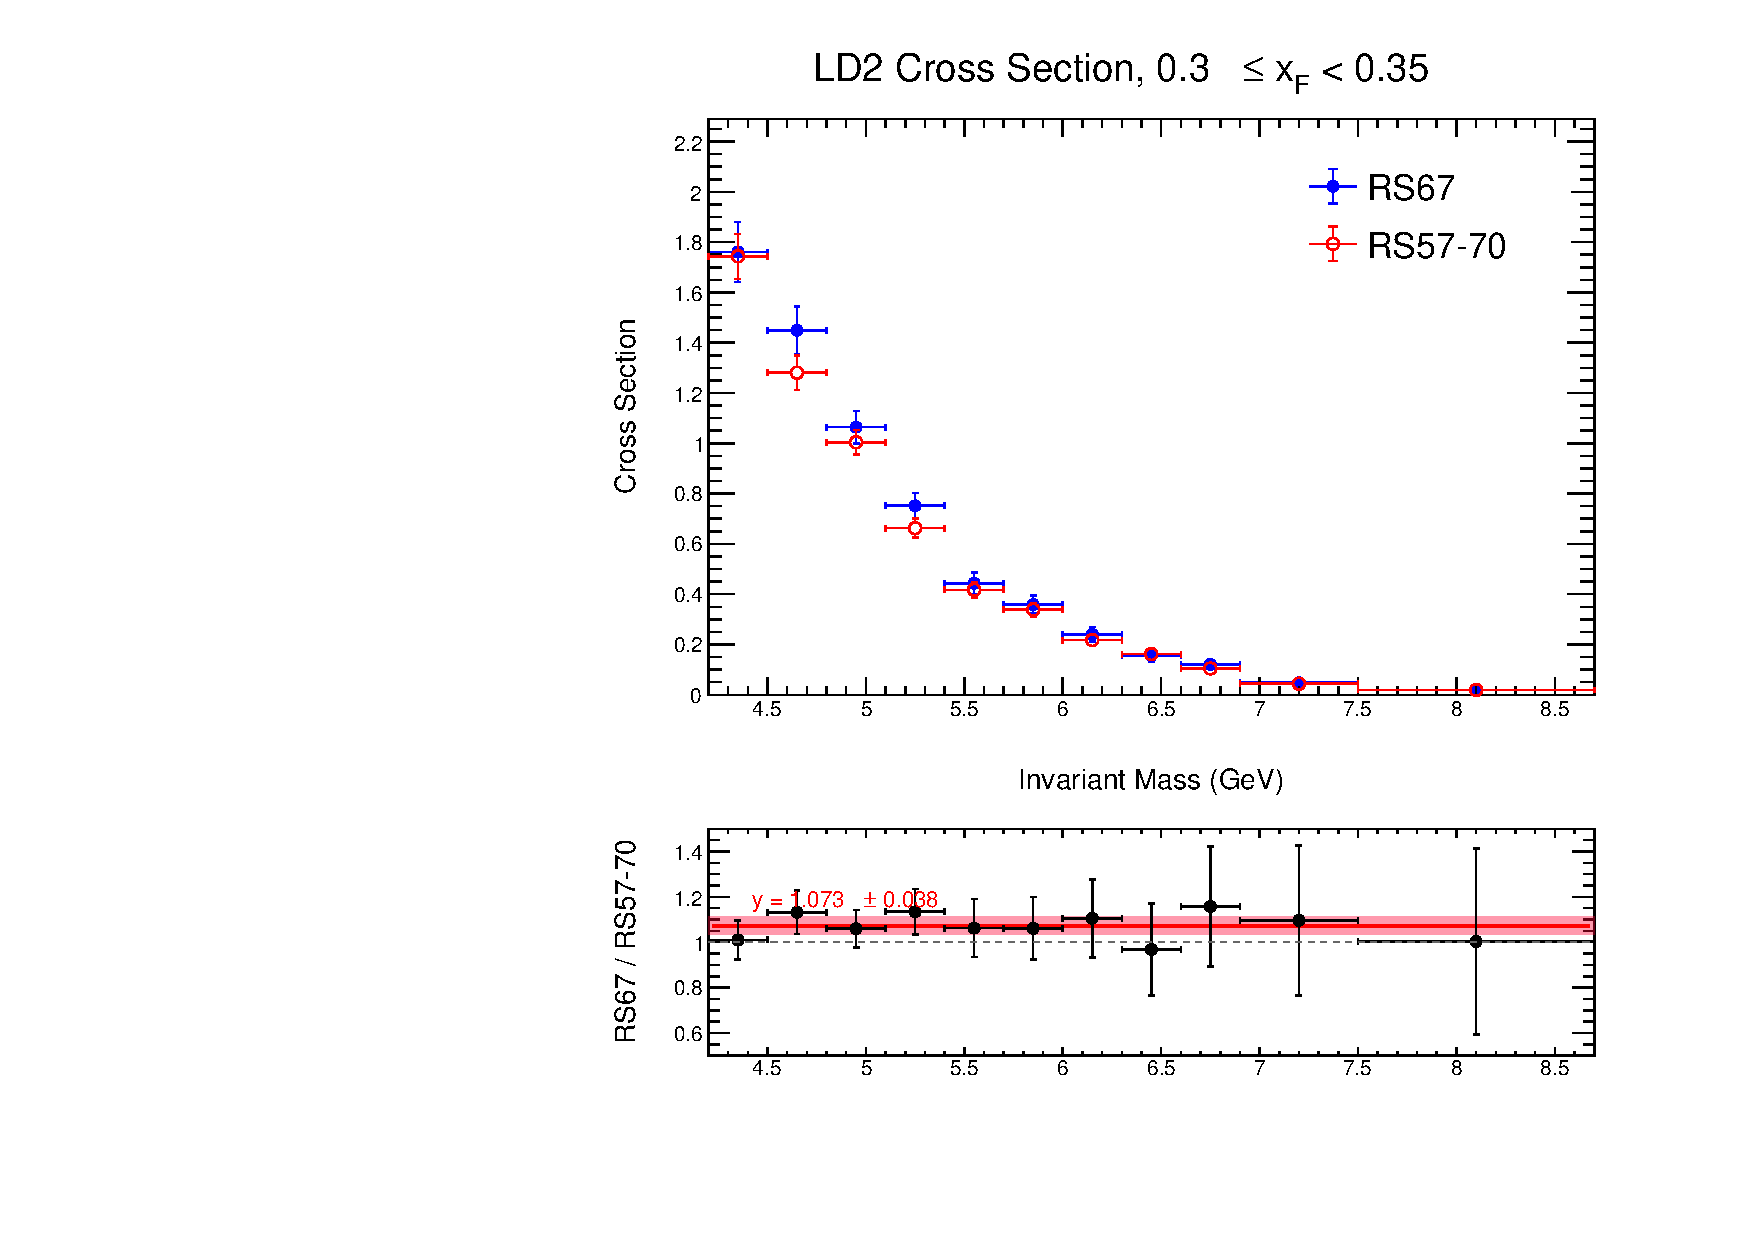
\includegraphics[width=\textwidth]{comparison_plots/XSec_Compare_LD2_xF_6.pdf}
    \end{column}
  \end{columns}
\end{frame}
\begin{frame}{Comparison for $0.35 \leq x_F < 0.4$}
  \begin{columns}
    \begin{column}{0.5\textwidth}
      \centering \textbf{Target: LH2}
      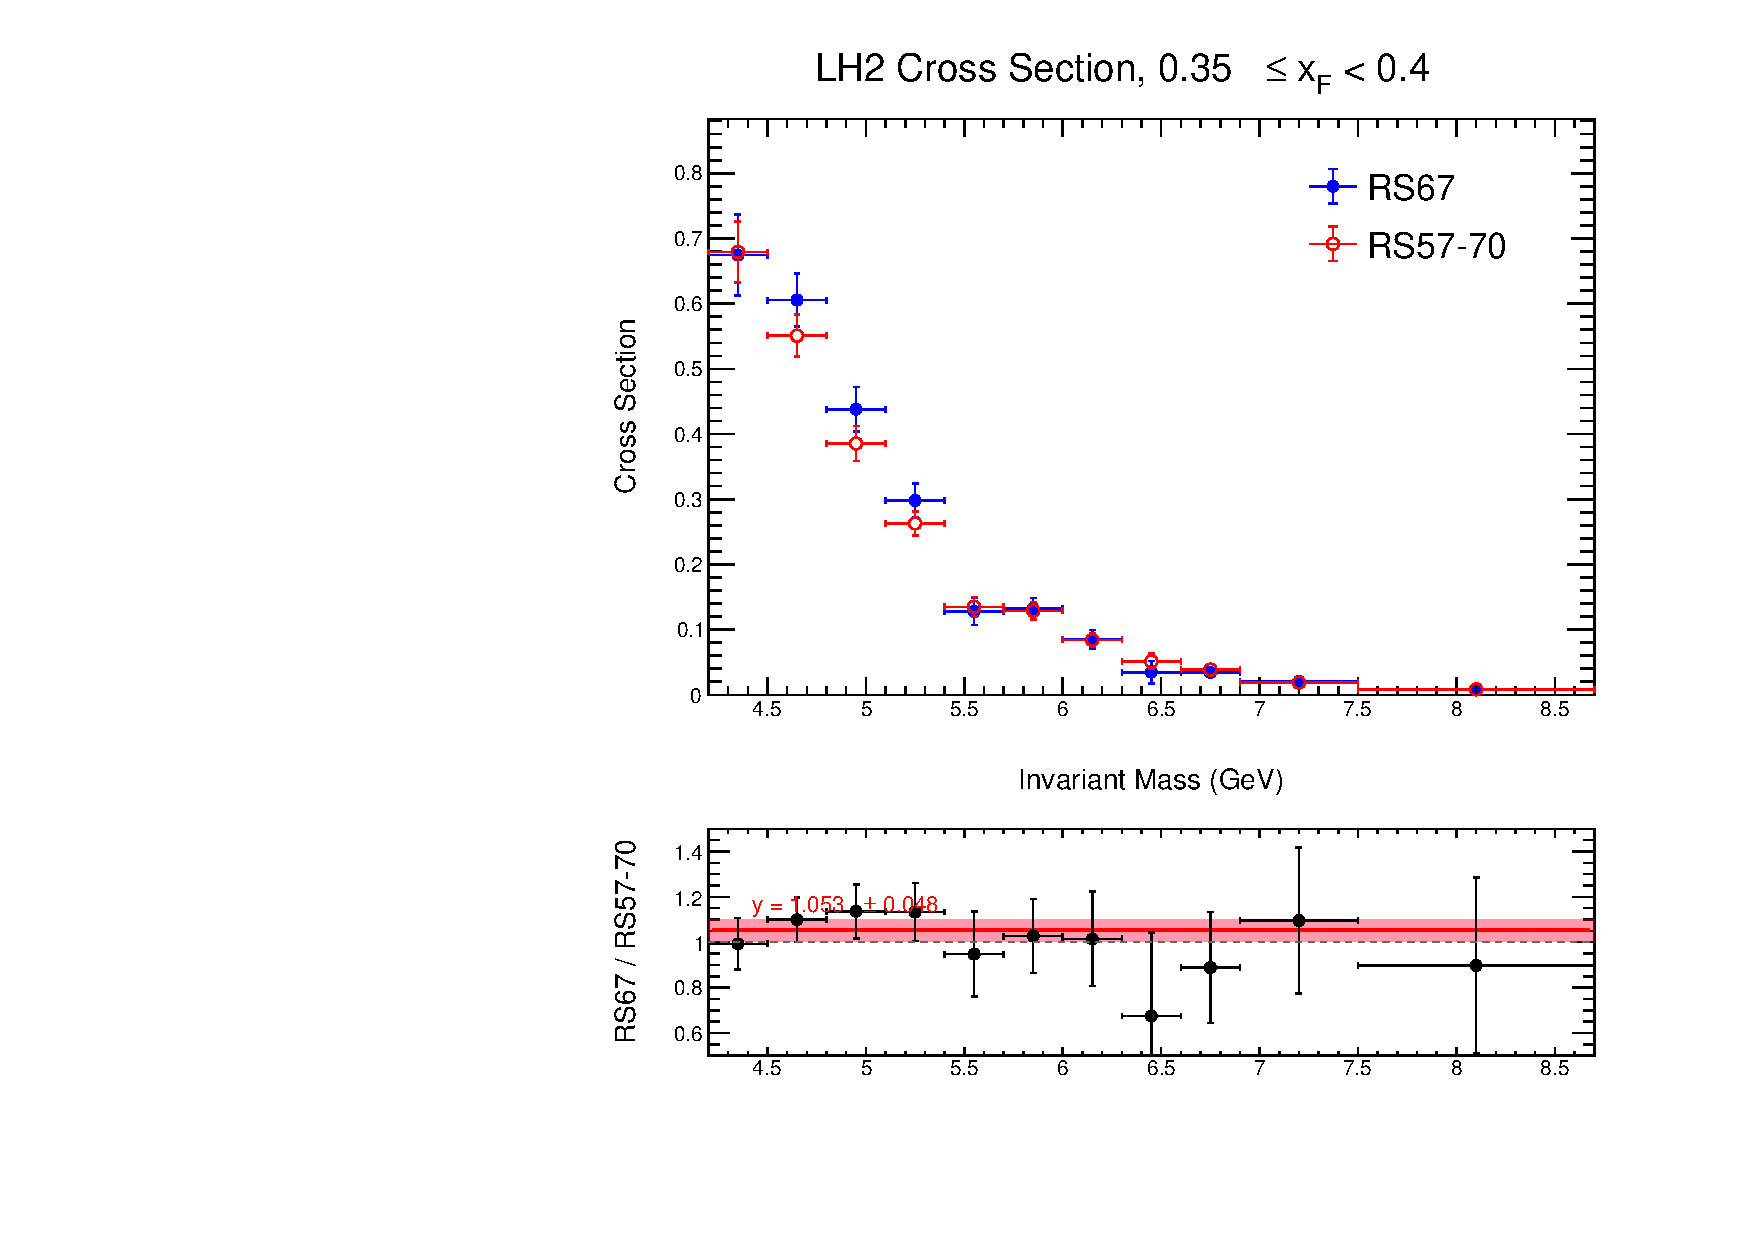
\includegraphics[width=\textwidth]{comparison_plots/XSec_Compare_LH2_xF_7.pdf}
    \end{column}
    \begin{column}{0.5\textwidth}
      \centering \textbf{Target: LD2}
      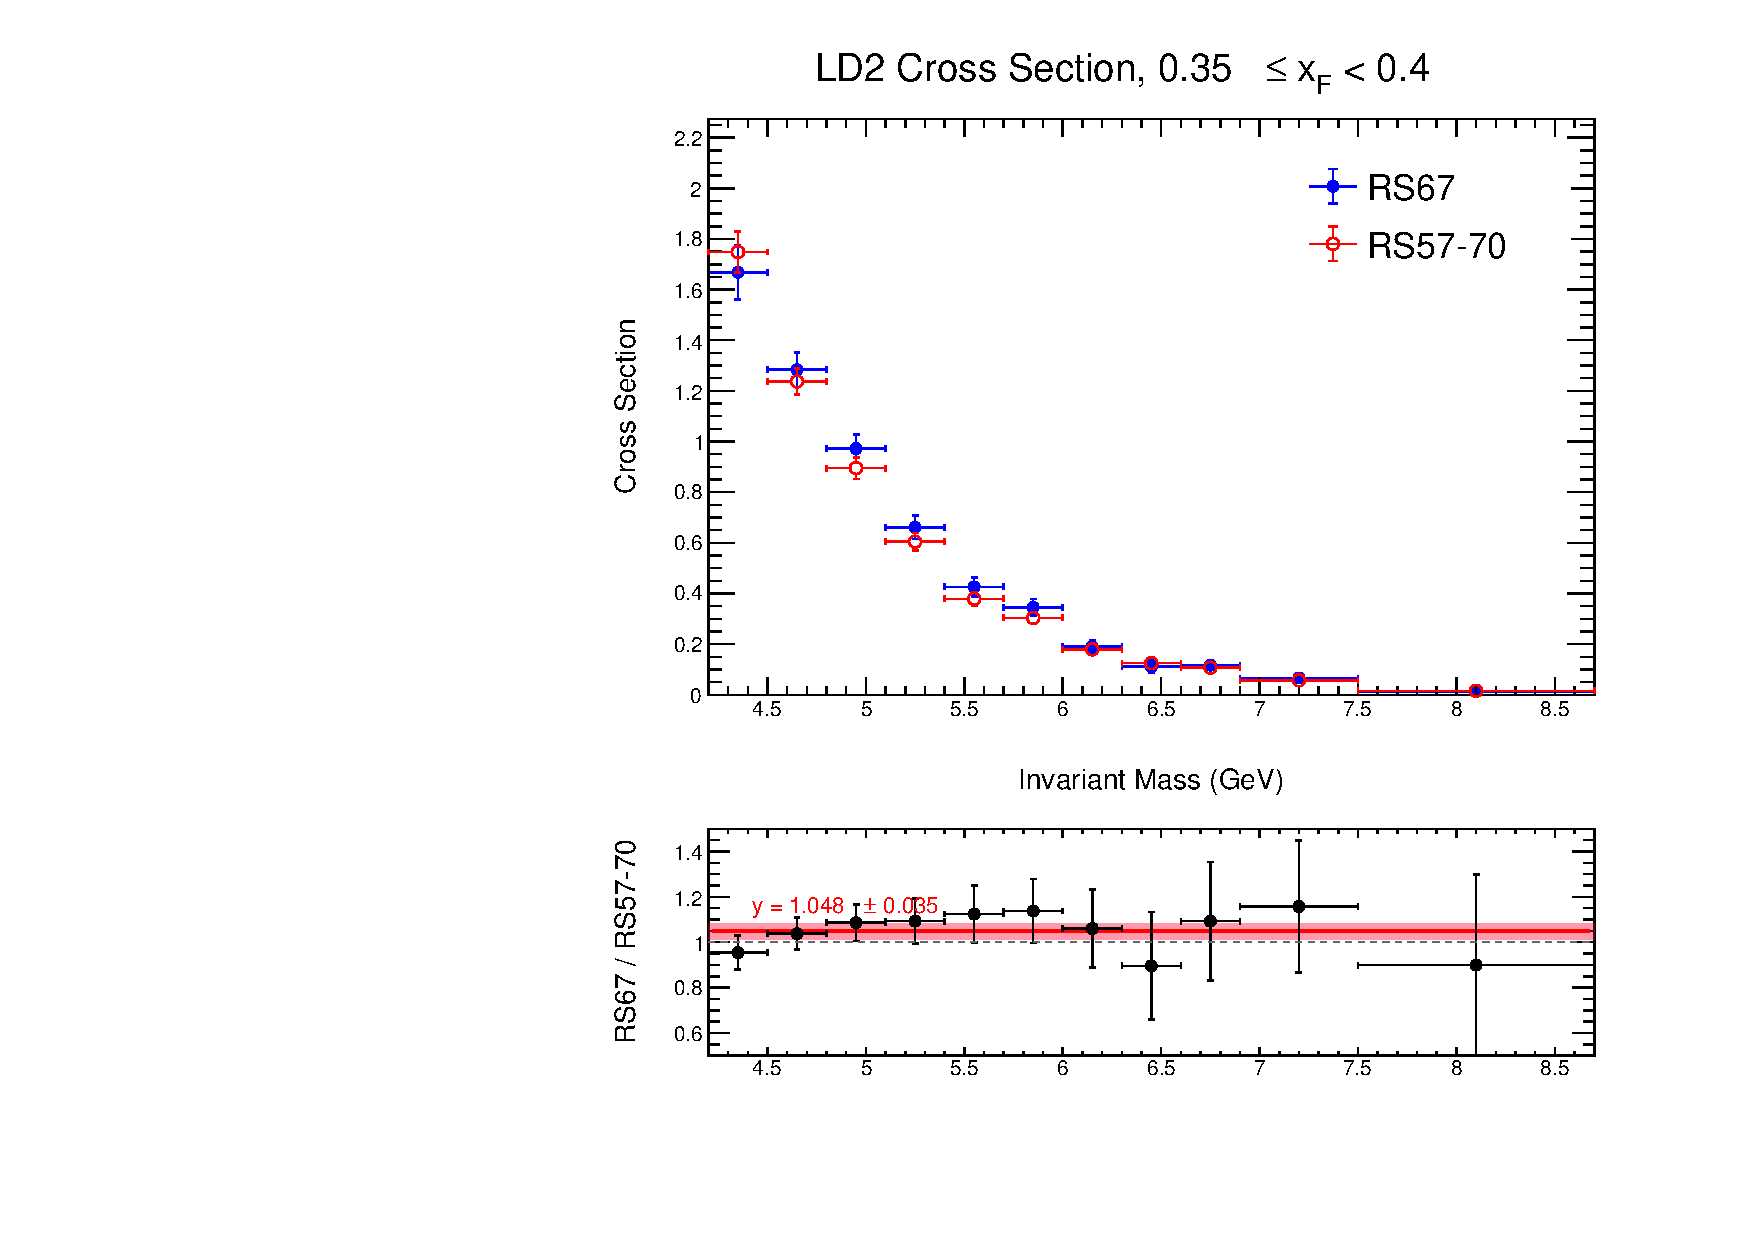
\includegraphics[width=\textwidth]{comparison_plots/XSec_Compare_LD2_xF_7.pdf}
    \end{column}
  \end{columns}
\end{frame}
\begin{frame}{Comparison for $0.4 \leq x_F < 0.45$}
  \begin{columns}
    \begin{column}{0.5\textwidth}
      \centering \textbf{Target: LH2}
      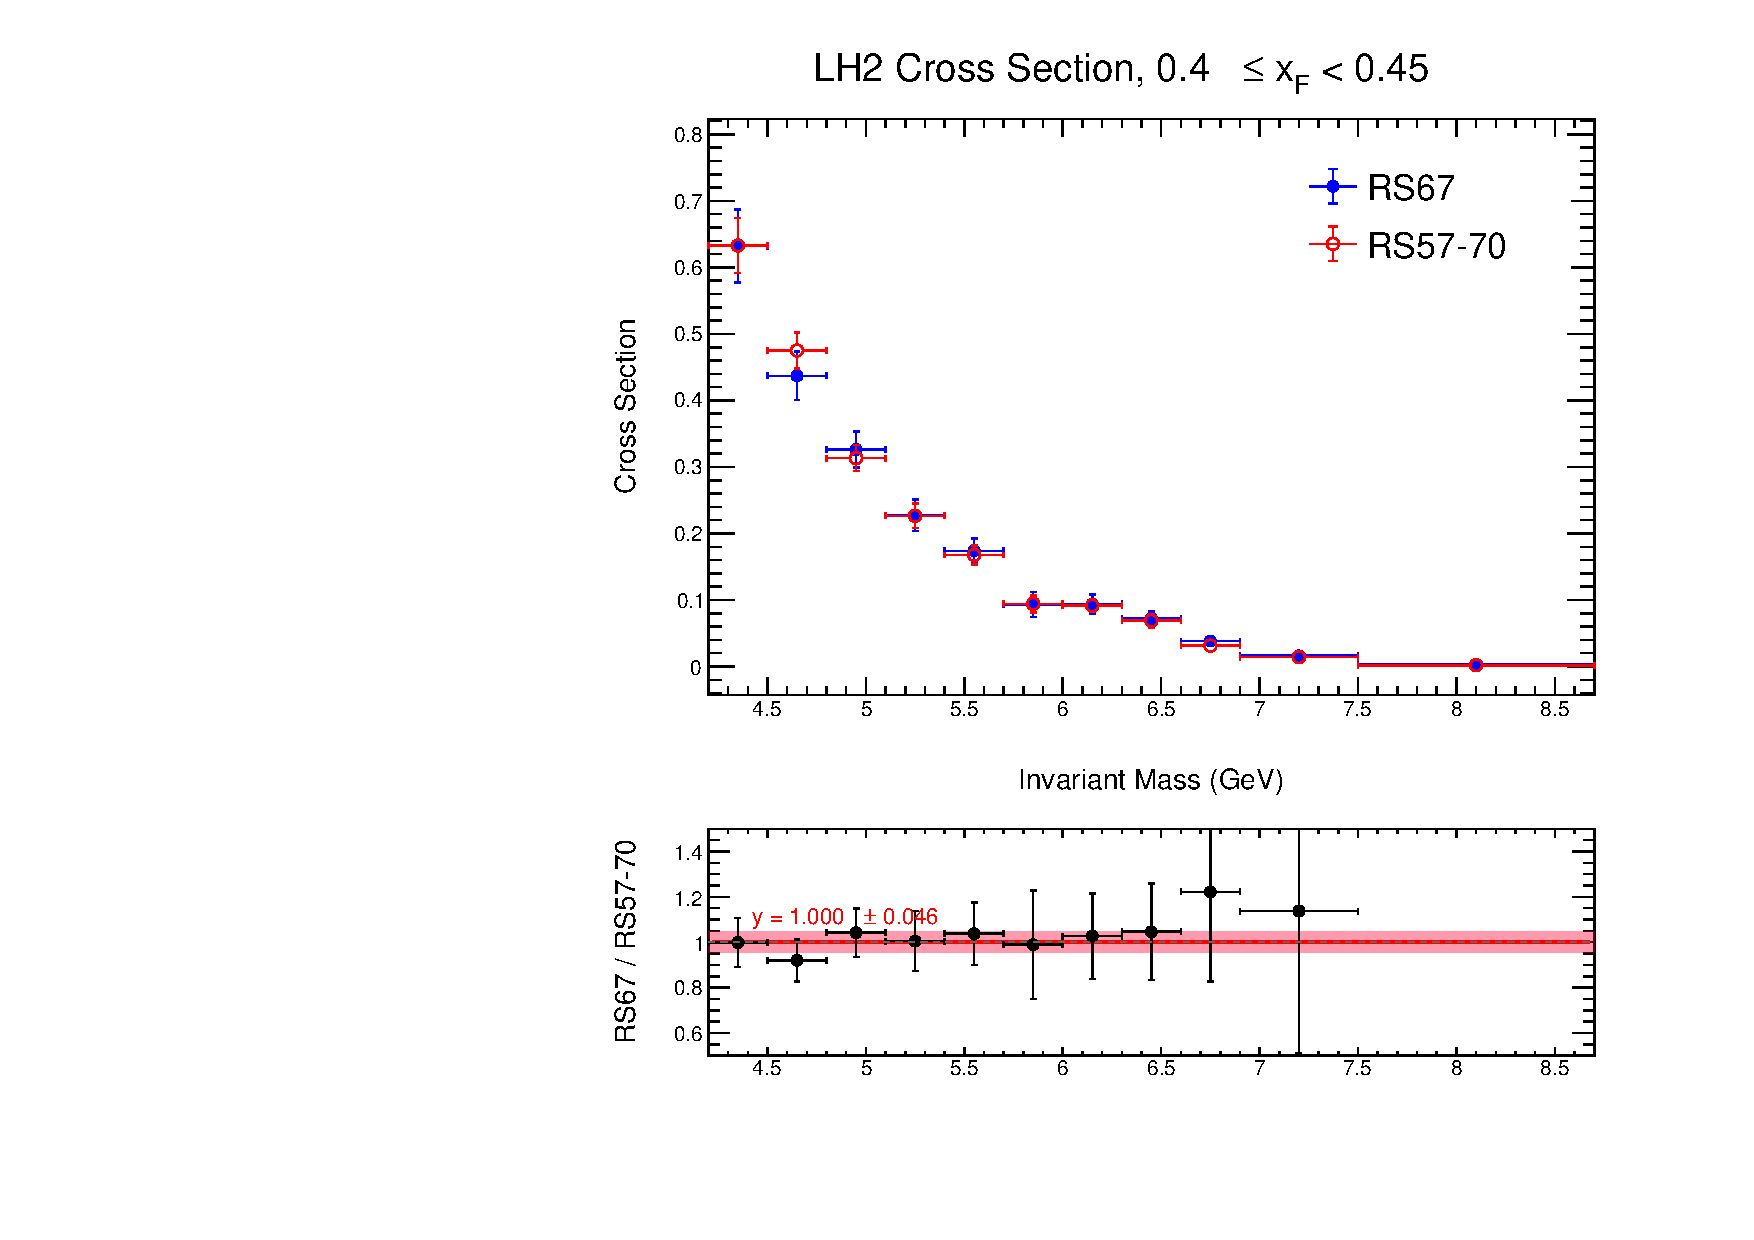
\includegraphics[width=\textwidth]{comparison_plots/XSec_Compare_LH2_xF_8.pdf}
    \end{column}
    \begin{column}{0.5\textwidth}
      \centering \textbf{Target: LD2}
      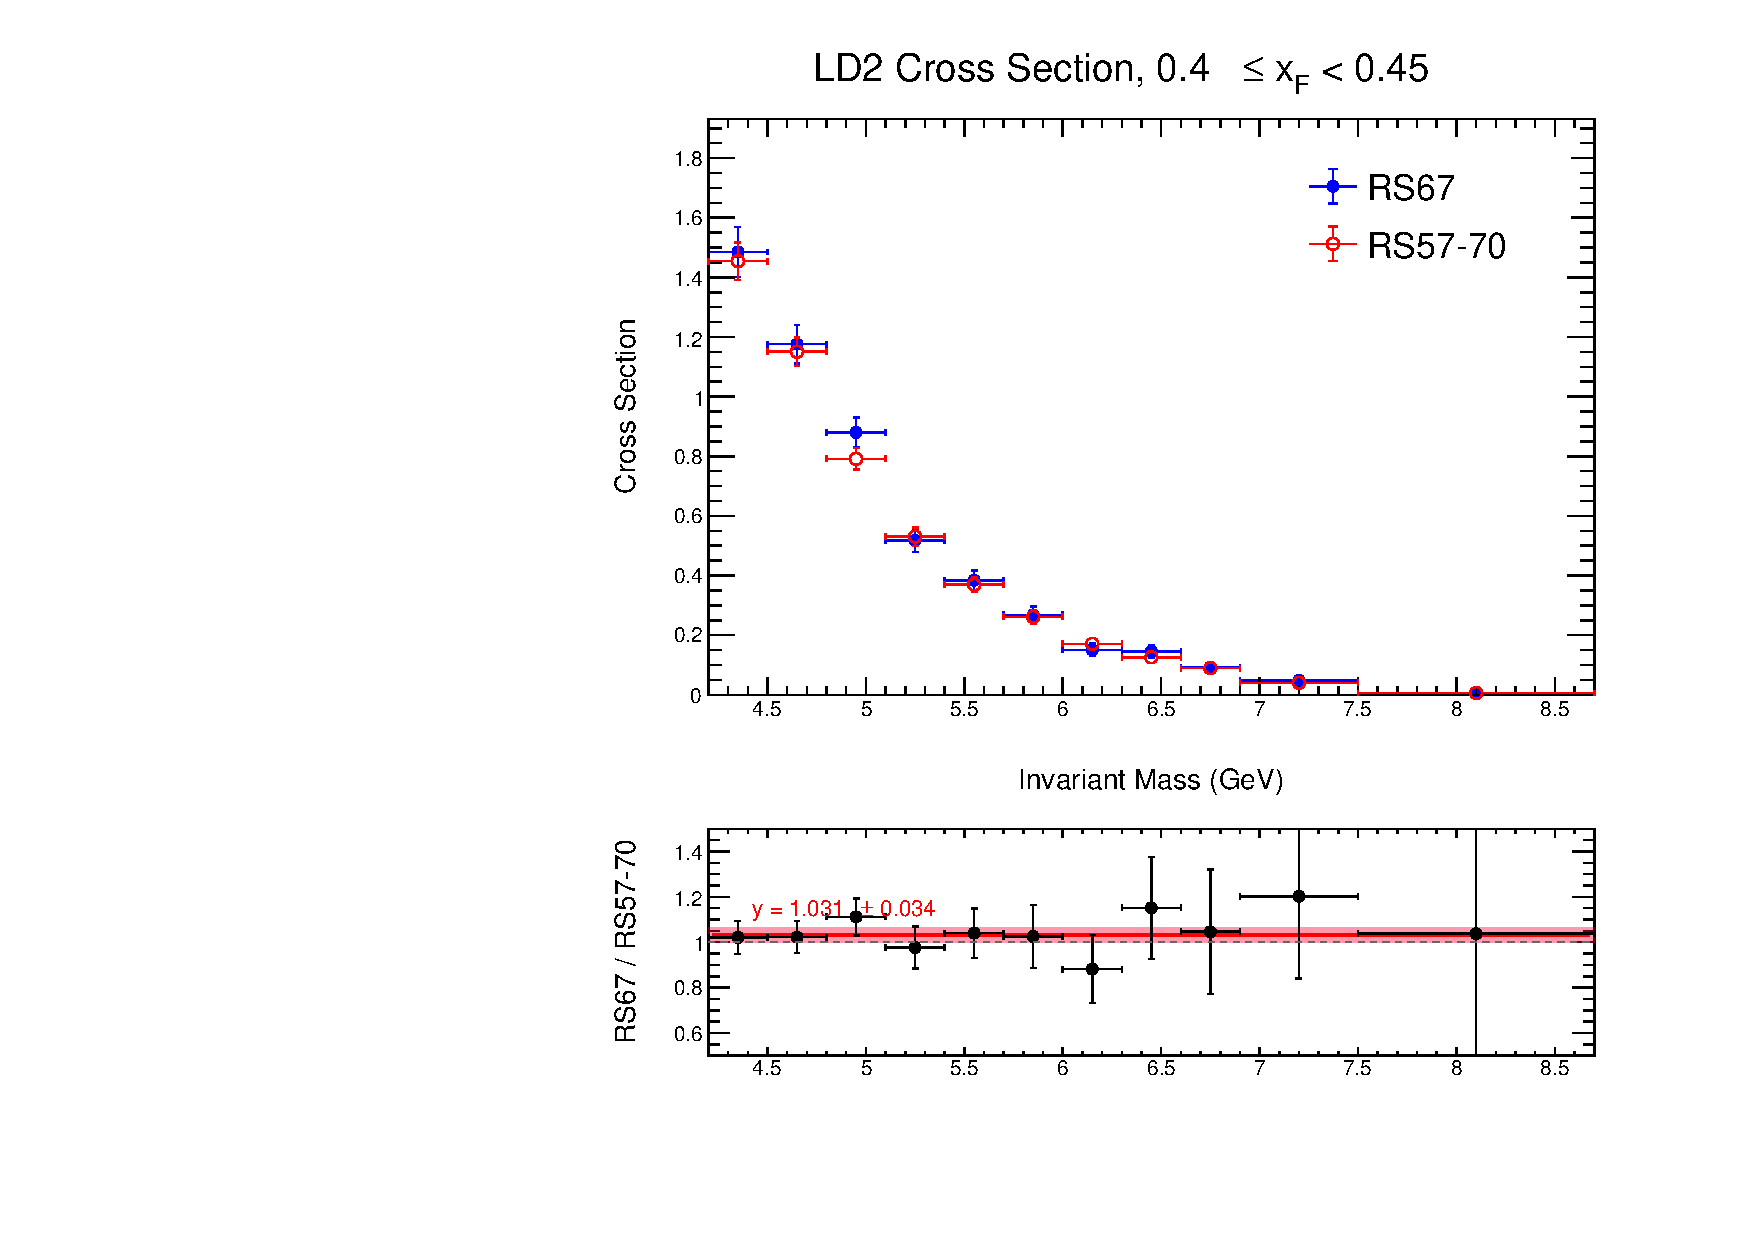
\includegraphics[width=\textwidth]{comparison_plots/XSec_Compare_LD2_xF_8.pdf}
    \end{column}
  \end{columns}
\end{frame}
\begin{frame}{Comparison for $0.45 \leq x_F < 0.5$}
  \begin{columns}
    \begin{column}{0.5\textwidth}
      \centering \textbf{Target: LH2}
      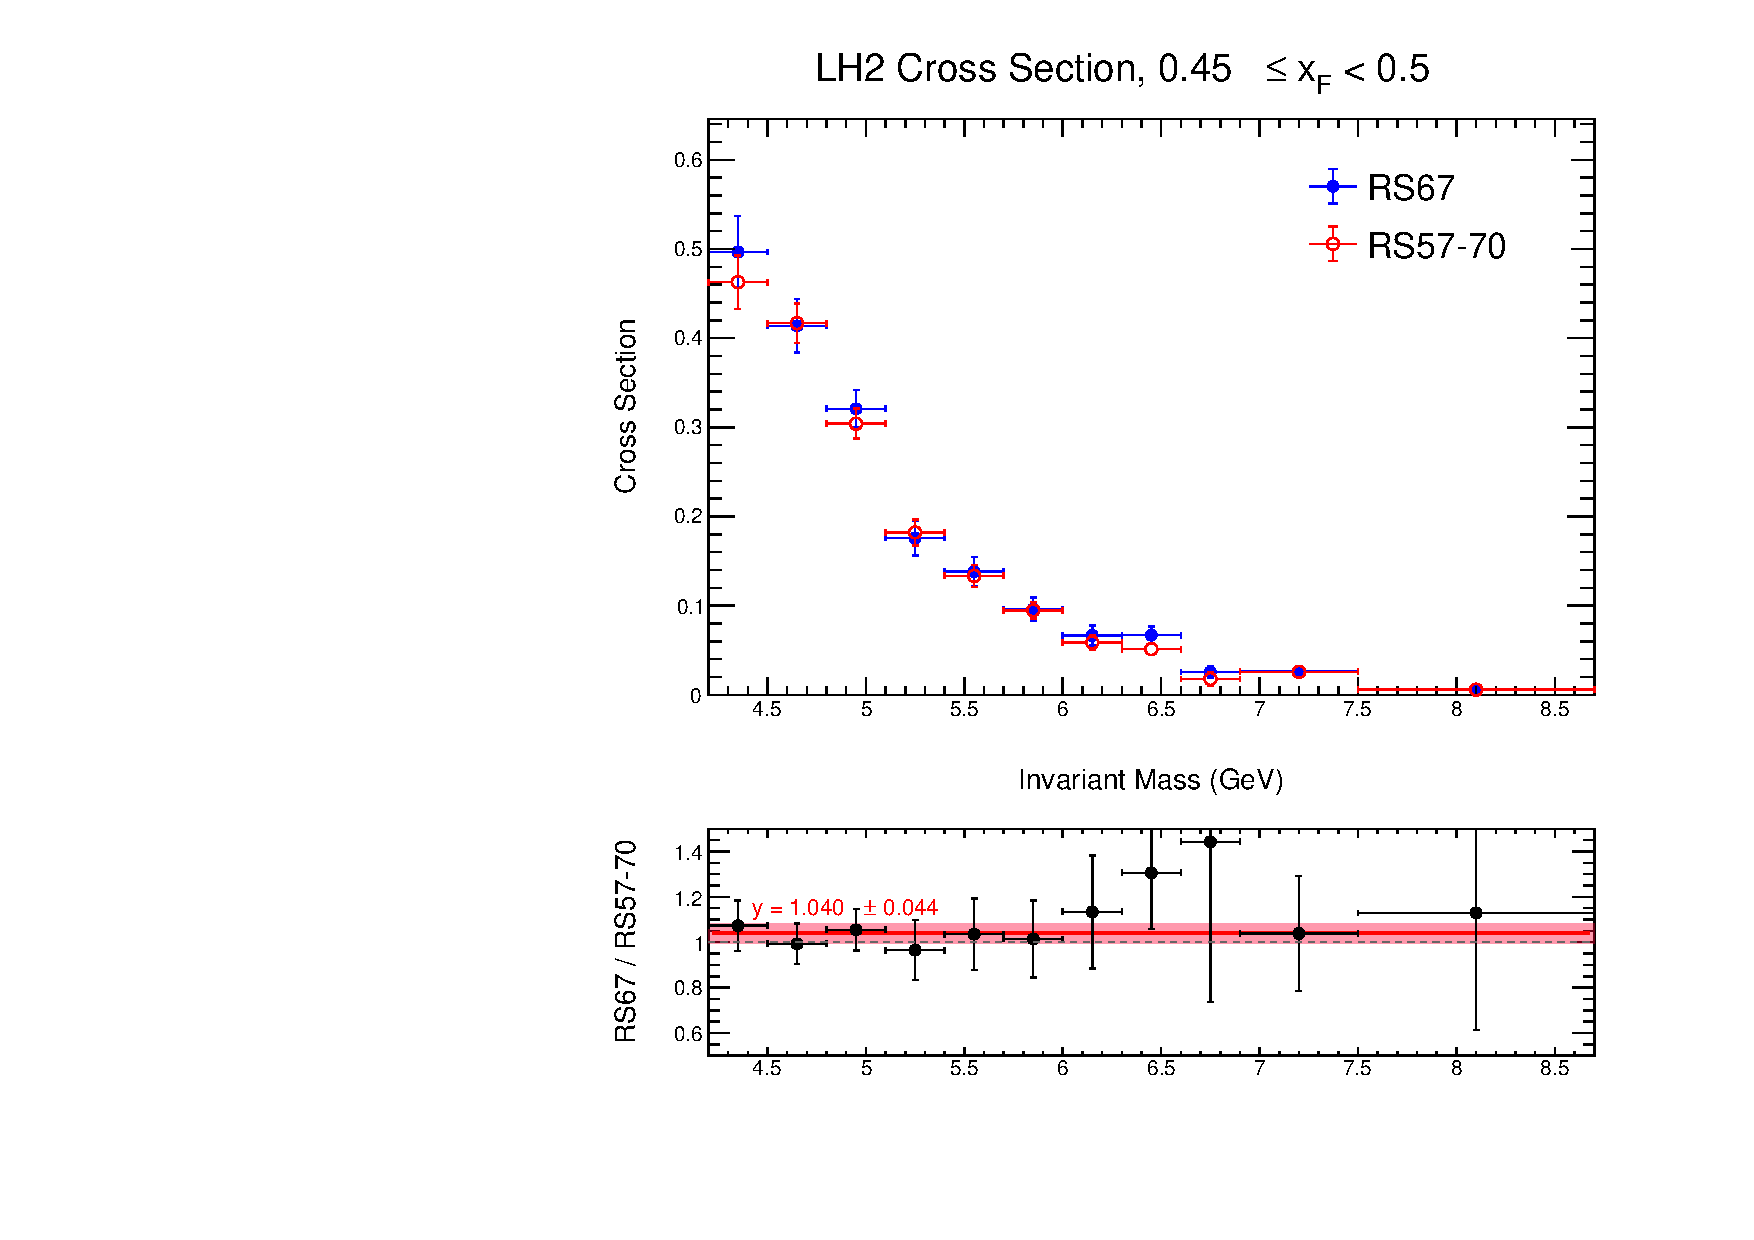
\includegraphics[width=\textwidth]{comparison_plots/XSec_Compare_LH2_xF_9.pdf}
    \end{column}
    \begin{column}{0.5\textwidth}
      \centering \textbf{Target: LD2}
      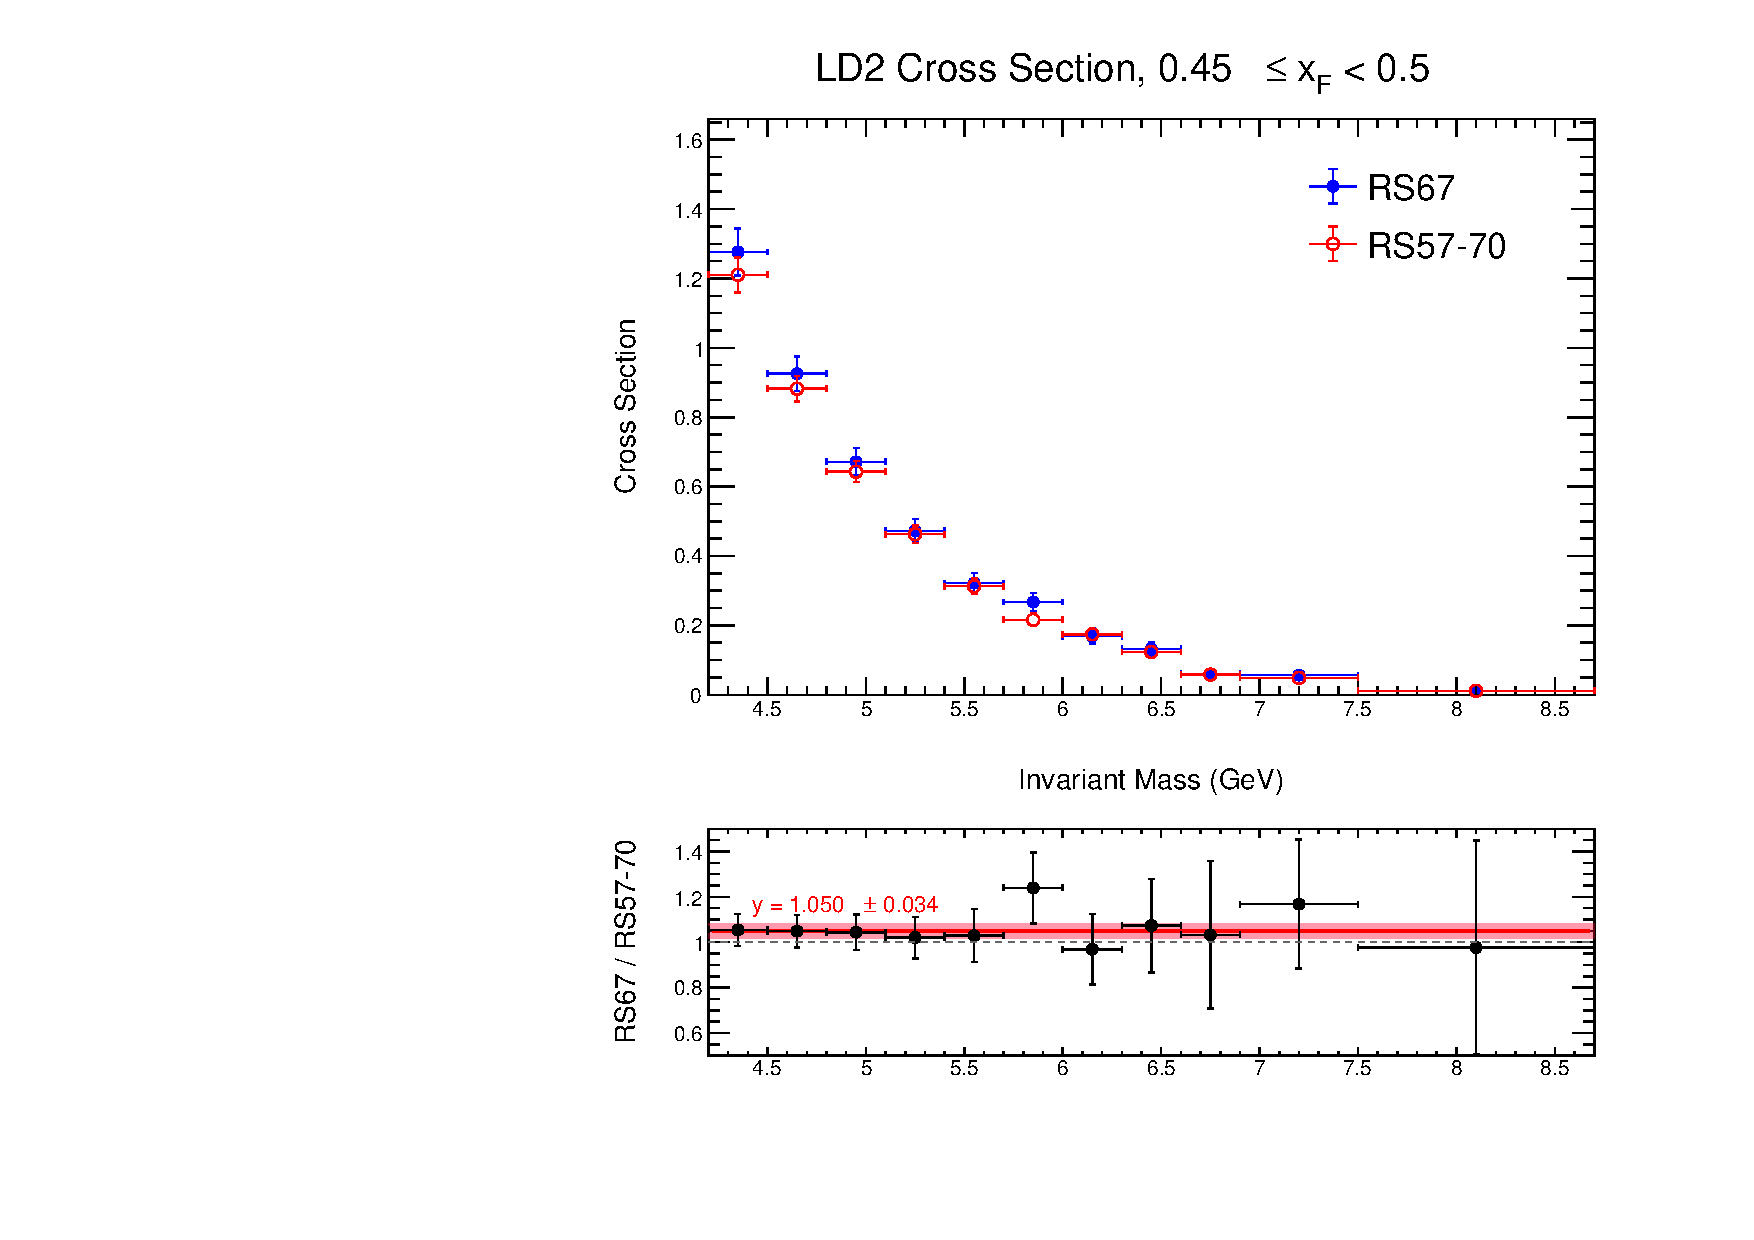
\includegraphics[width=\textwidth]{comparison_plots/XSec_Compare_LD2_xF_9.pdf}
    \end{column}
  \end{columns}
\end{frame}
\begin{frame}{Comparison for $0.5 \leq x_F < 0.55$}
  \begin{columns}
    \begin{column}{0.5\textwidth}
      \centering \textbf{Target: LH2}
      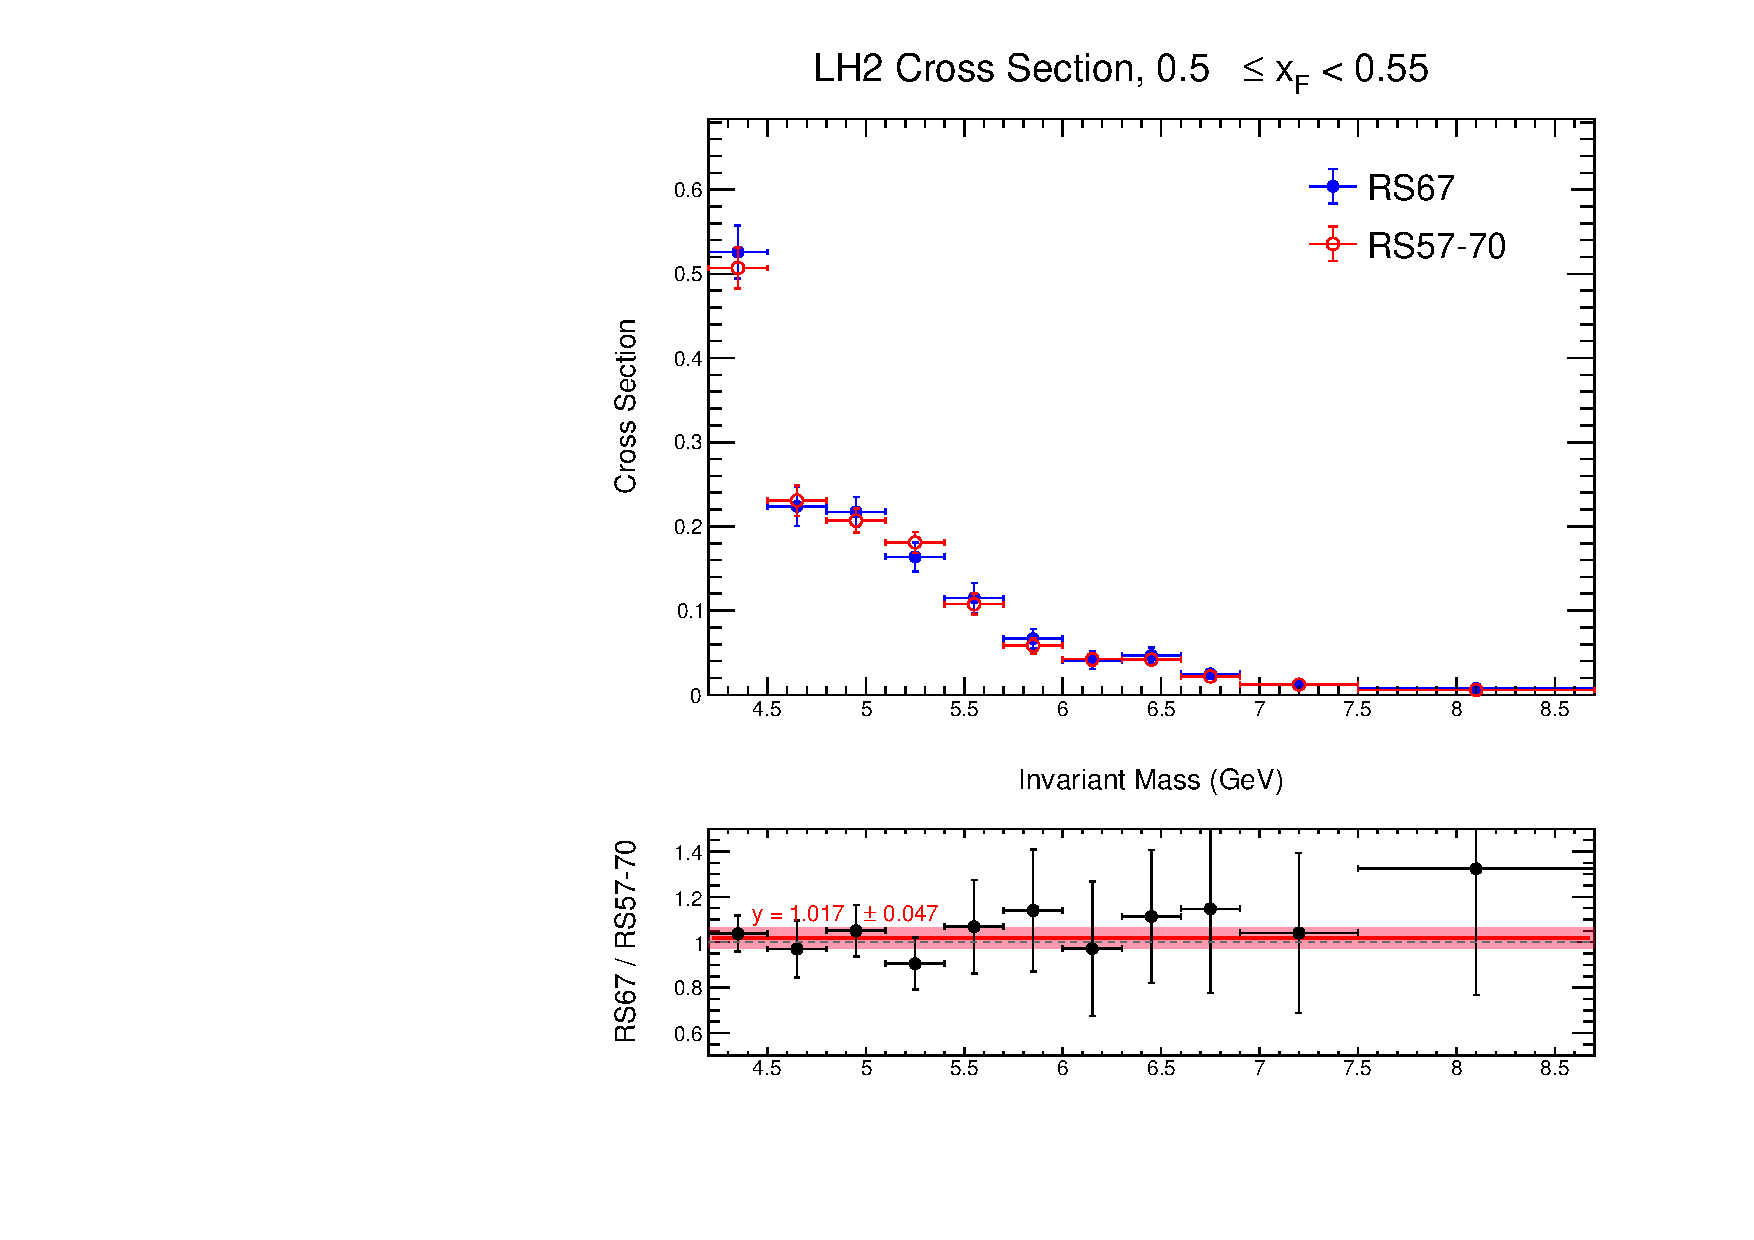
\includegraphics[width=\textwidth]{comparison_plots/XSec_Compare_LH2_xF_10.pdf}
    \end{column}
    \begin{column}{0.5\textwidth}
      \centering \textbf{Target: LD2}
      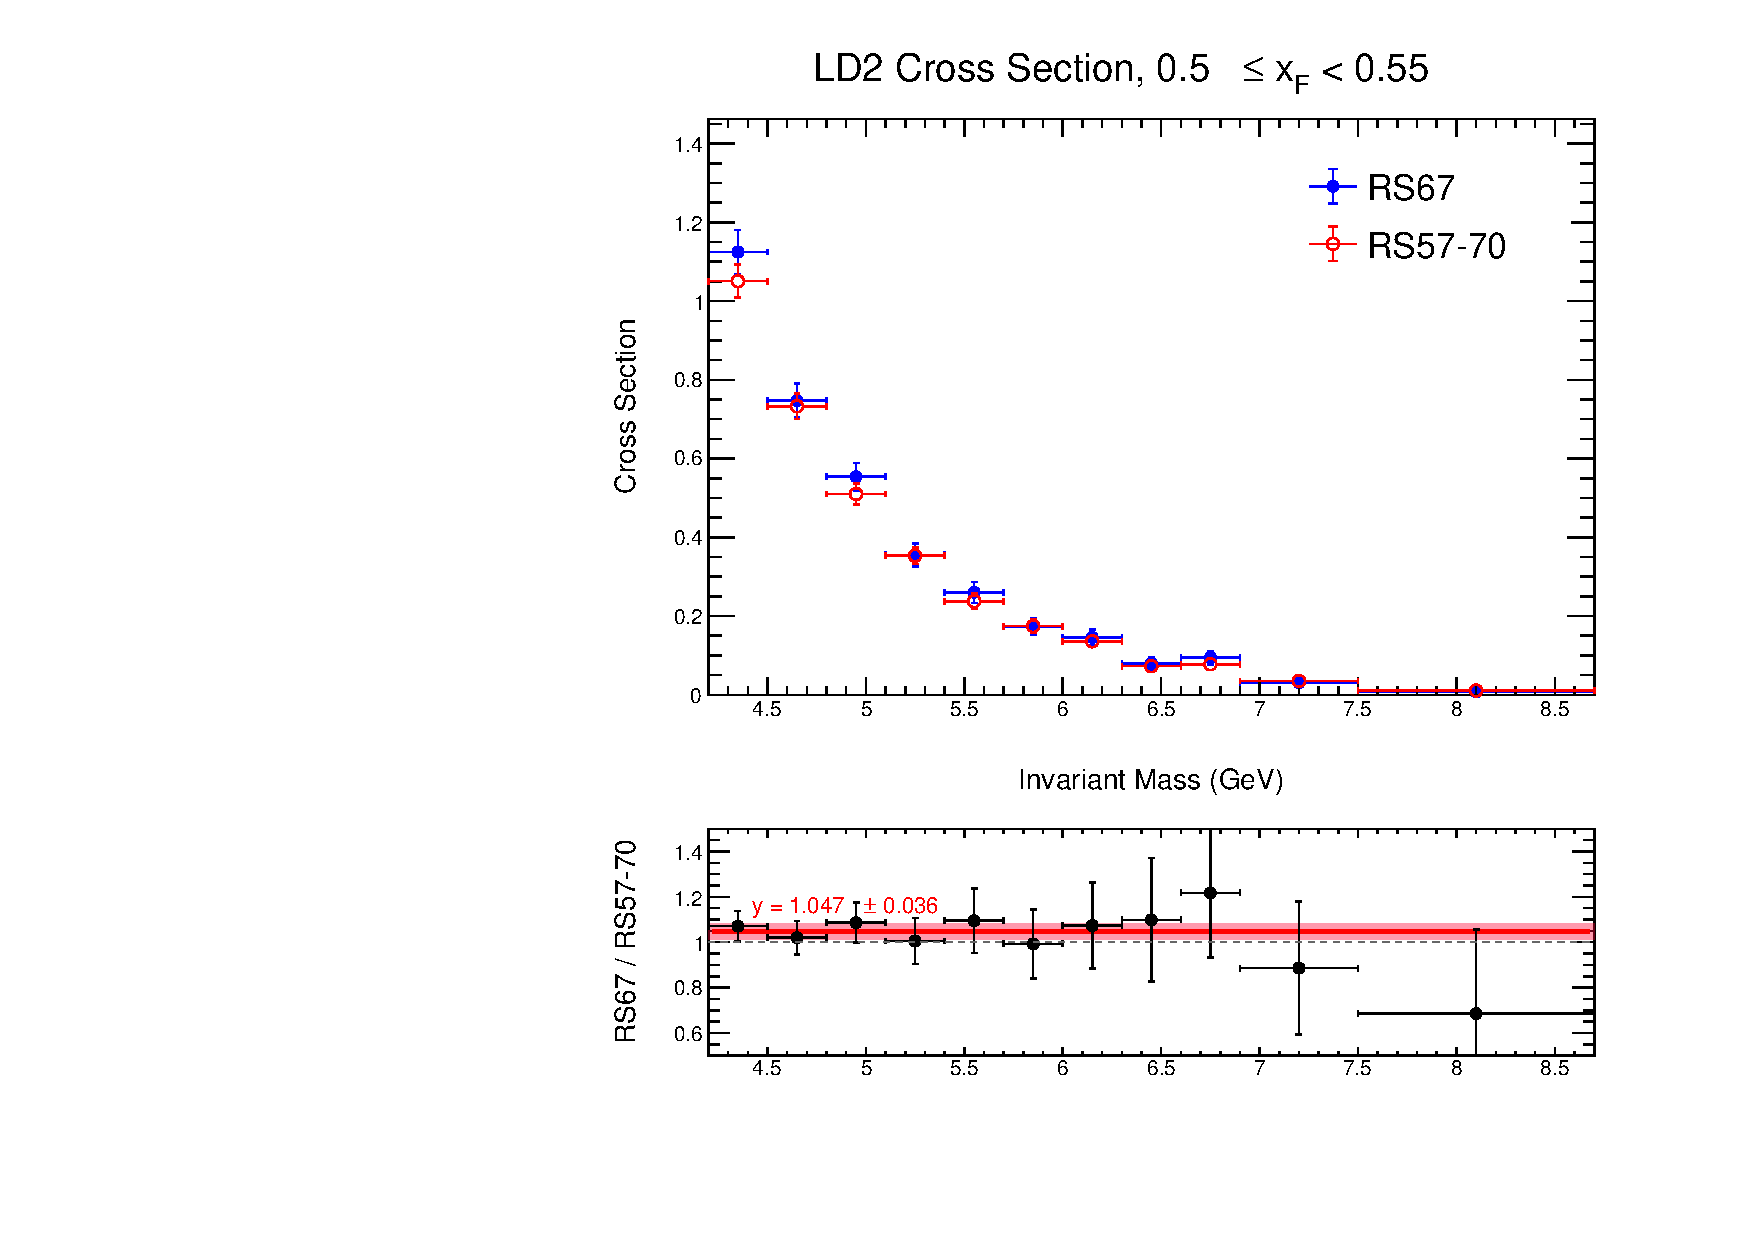
\includegraphics[width=\textwidth]{comparison_plots/XSec_Compare_LD2_xF_10.pdf}
    \end{column}
  \end{columns}
\end{frame}
\begin{frame}{Comparison for $0.55 \leq x_F < 0.6$}
  \begin{columns}
    \begin{column}{0.5\textwidth}
      \centering \textbf{Target: LH2}
      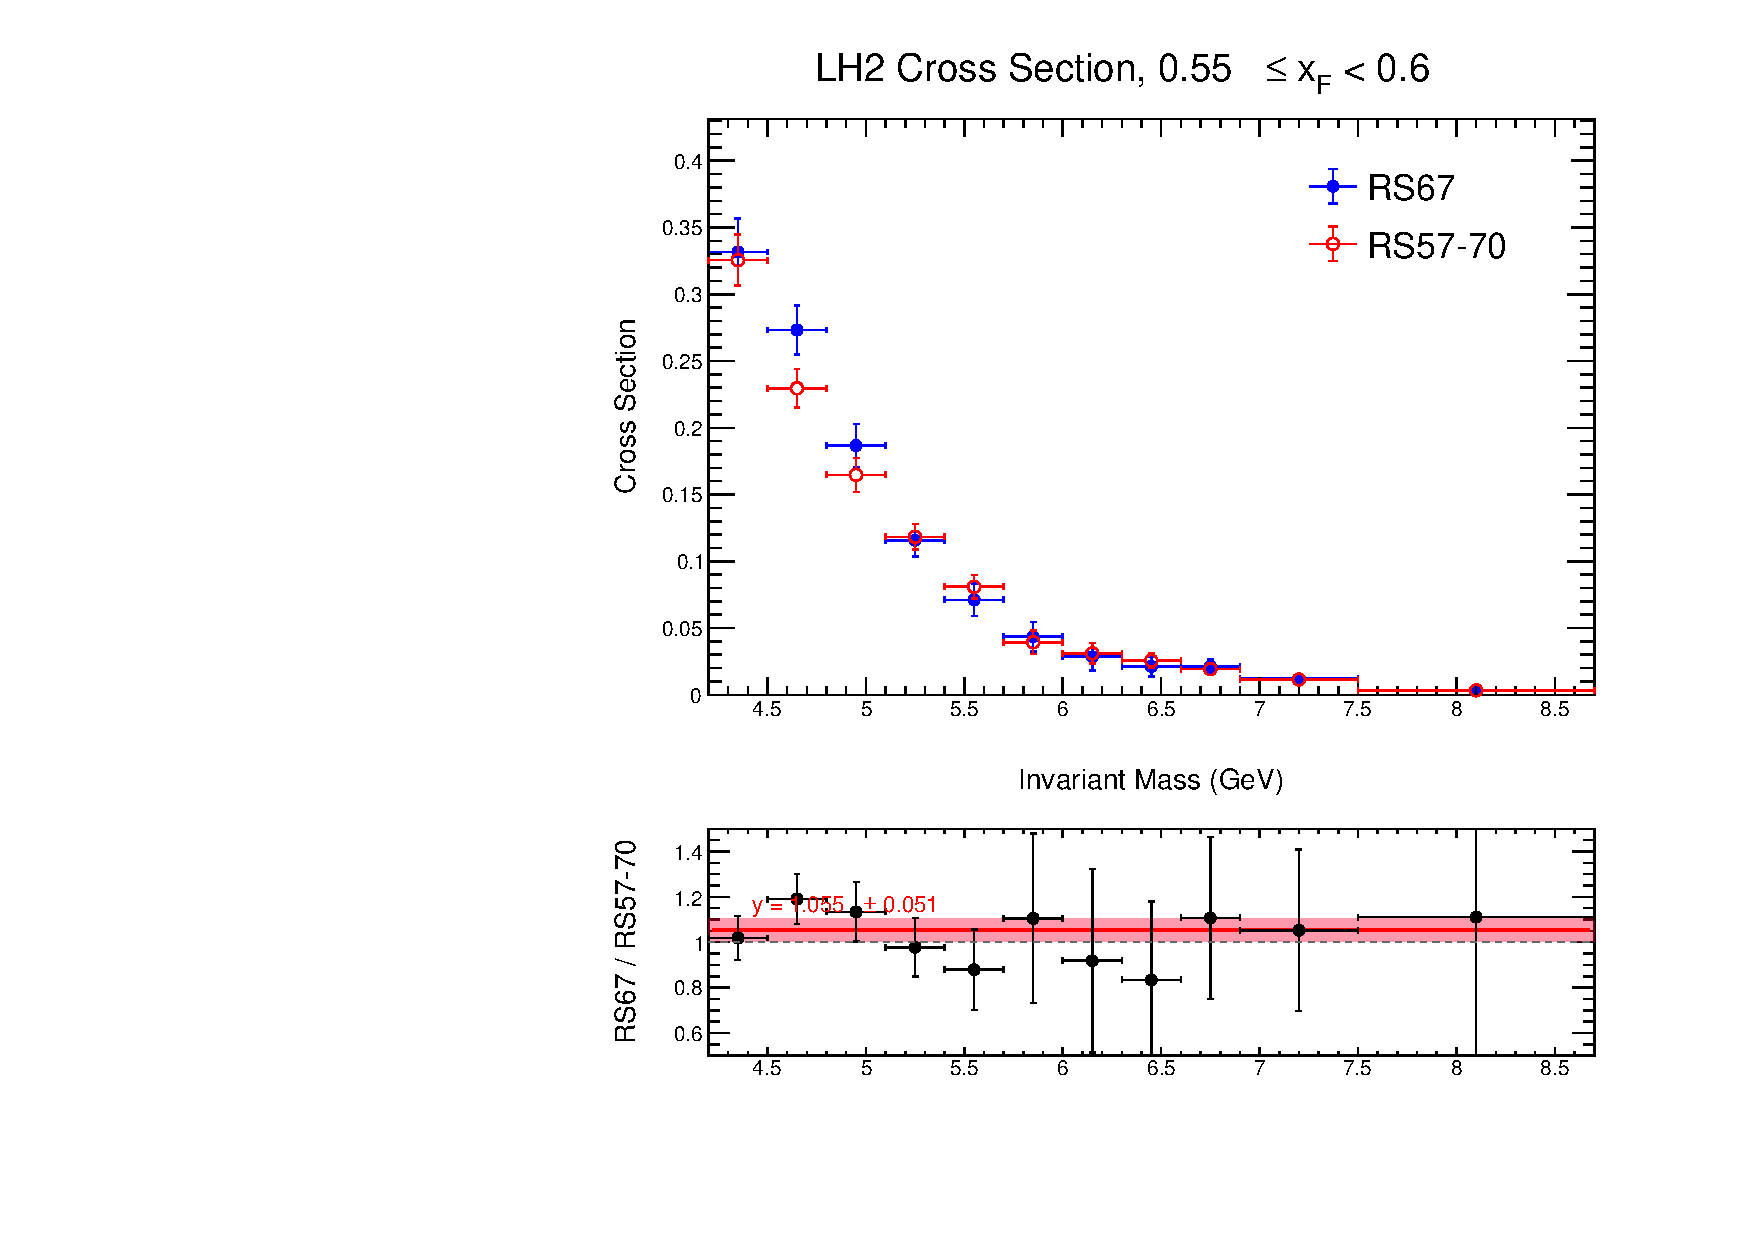
\includegraphics[width=\textwidth]{comparison_plots/XSec_Compare_LH2_xF_11.pdf}
    \end{column}
    \begin{column}{0.5\textwidth}
      \centering \textbf{Target: LD2}
      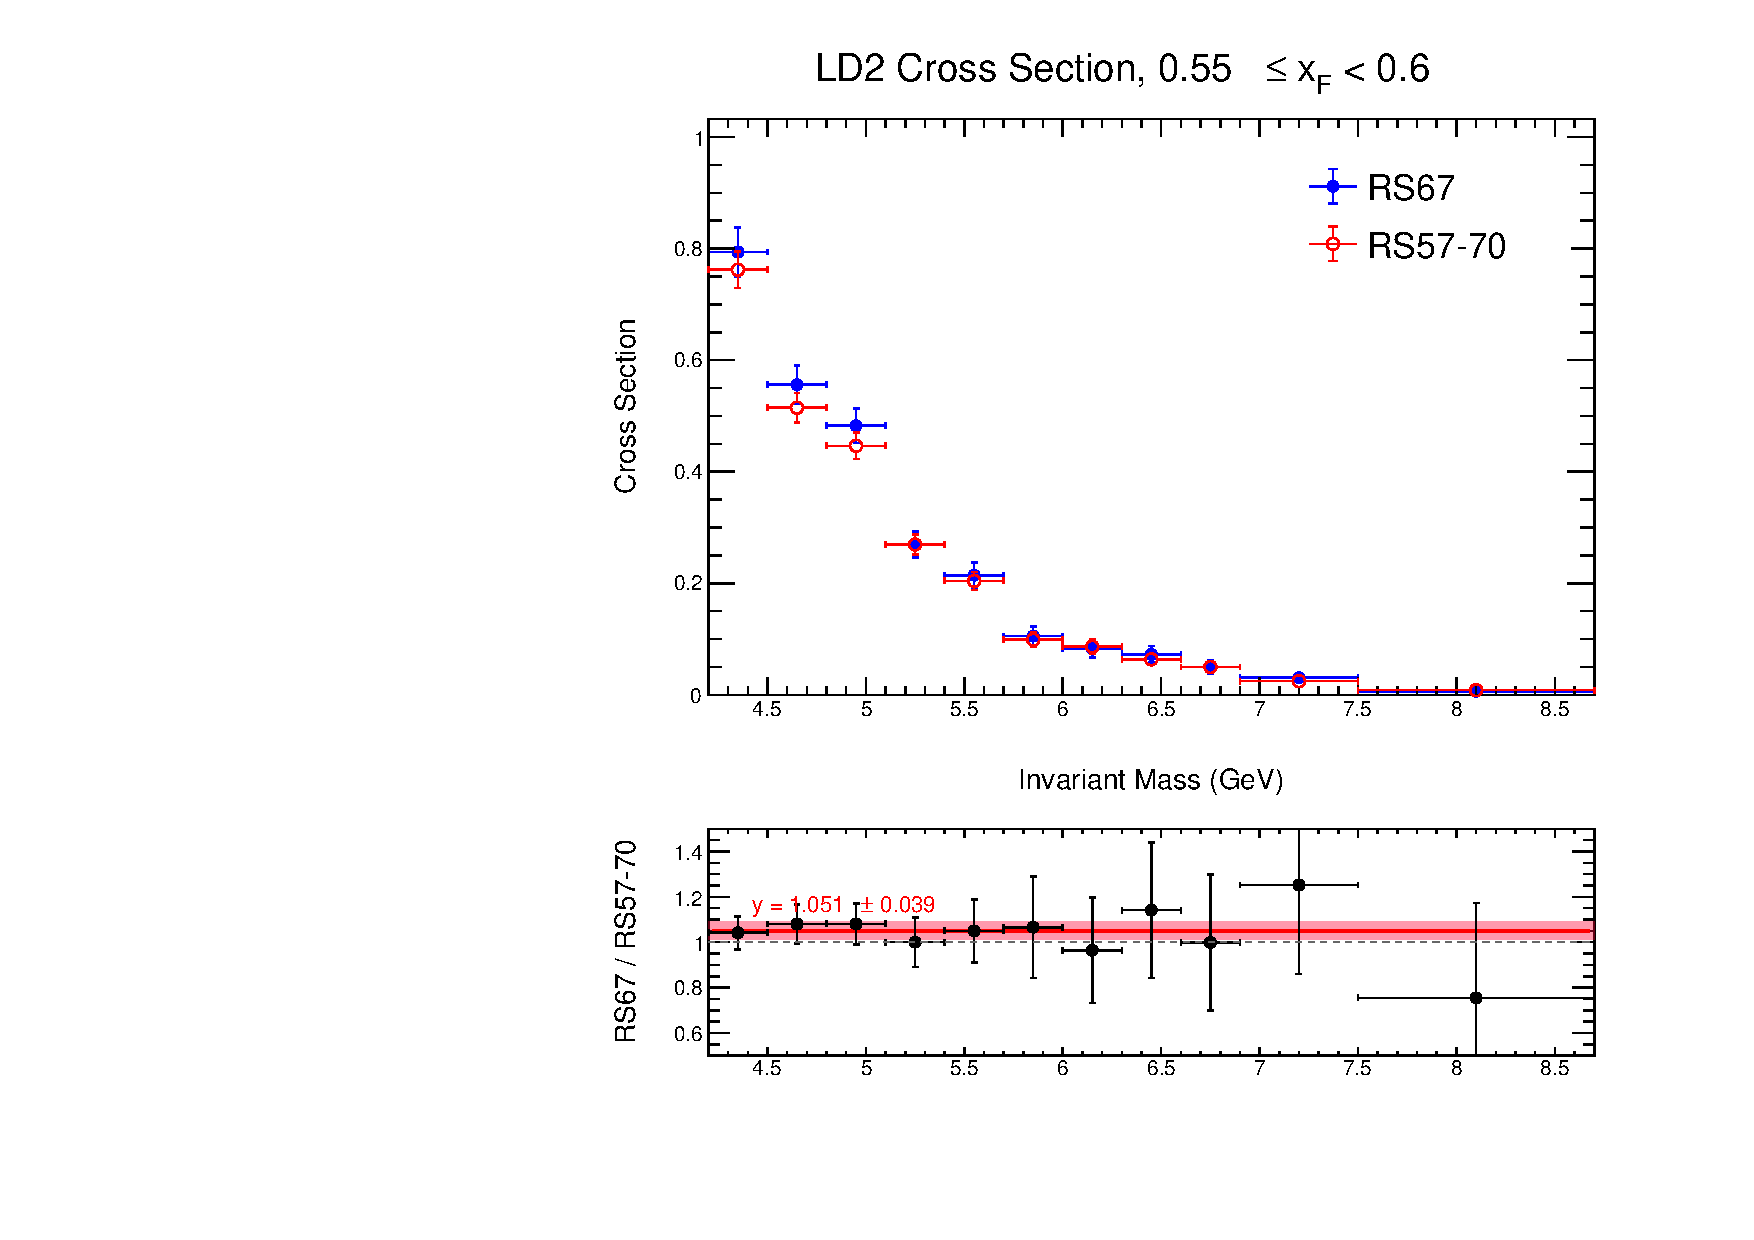
\includegraphics[width=\textwidth]{comparison_plots/XSec_Compare_LD2_xF_11.pdf}
    \end{column}
  \end{columns}
\end{frame}
\begin{frame}{Comparison for $0.6 \leq x_F < 0.65$}
  \begin{columns}
    \begin{column}{0.5\textwidth}
      \centering \textbf{Target: LH2}
      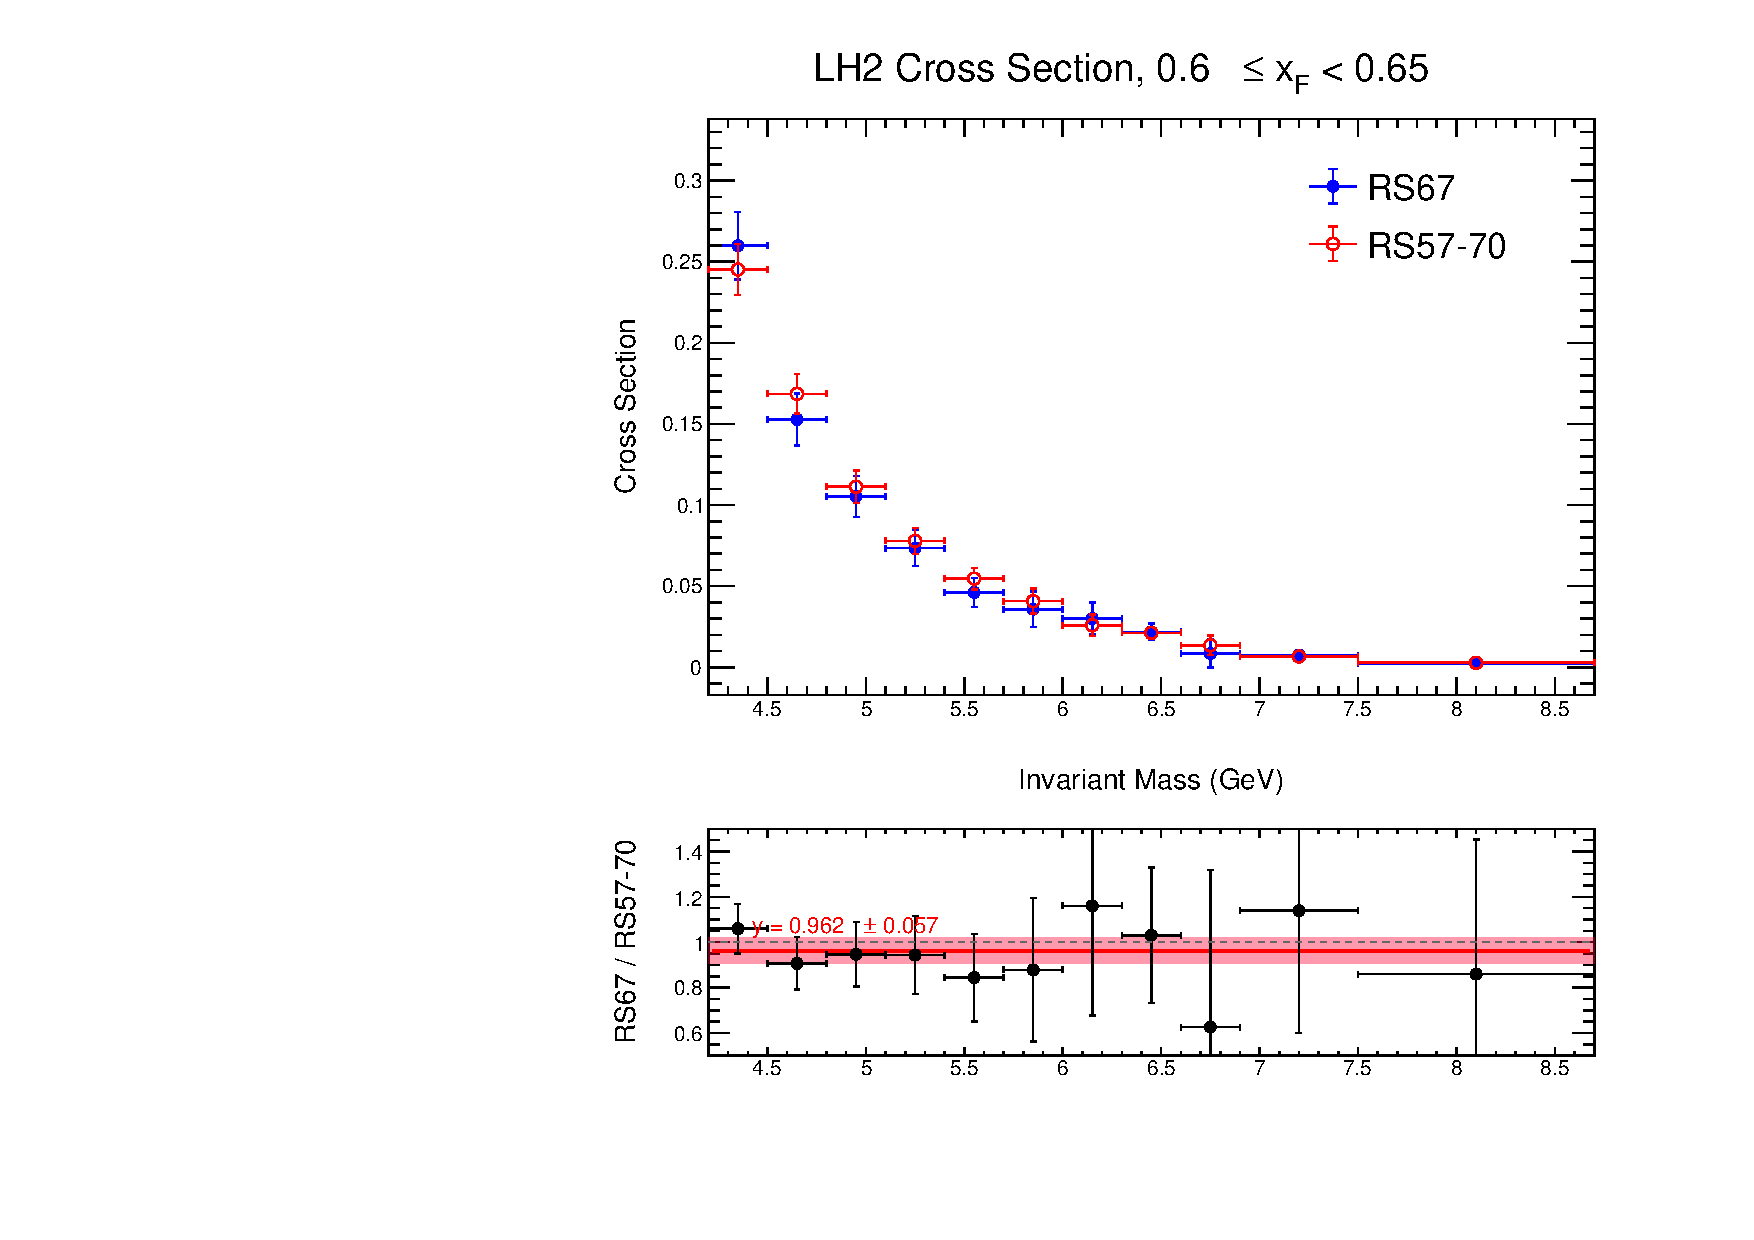
\includegraphics[width=\textwidth]{comparison_plots/XSec_Compare_LH2_xF_12.pdf}
    \end{column}
    \begin{column}{0.5\textwidth}
      \centering \textbf{Target: LD2}
      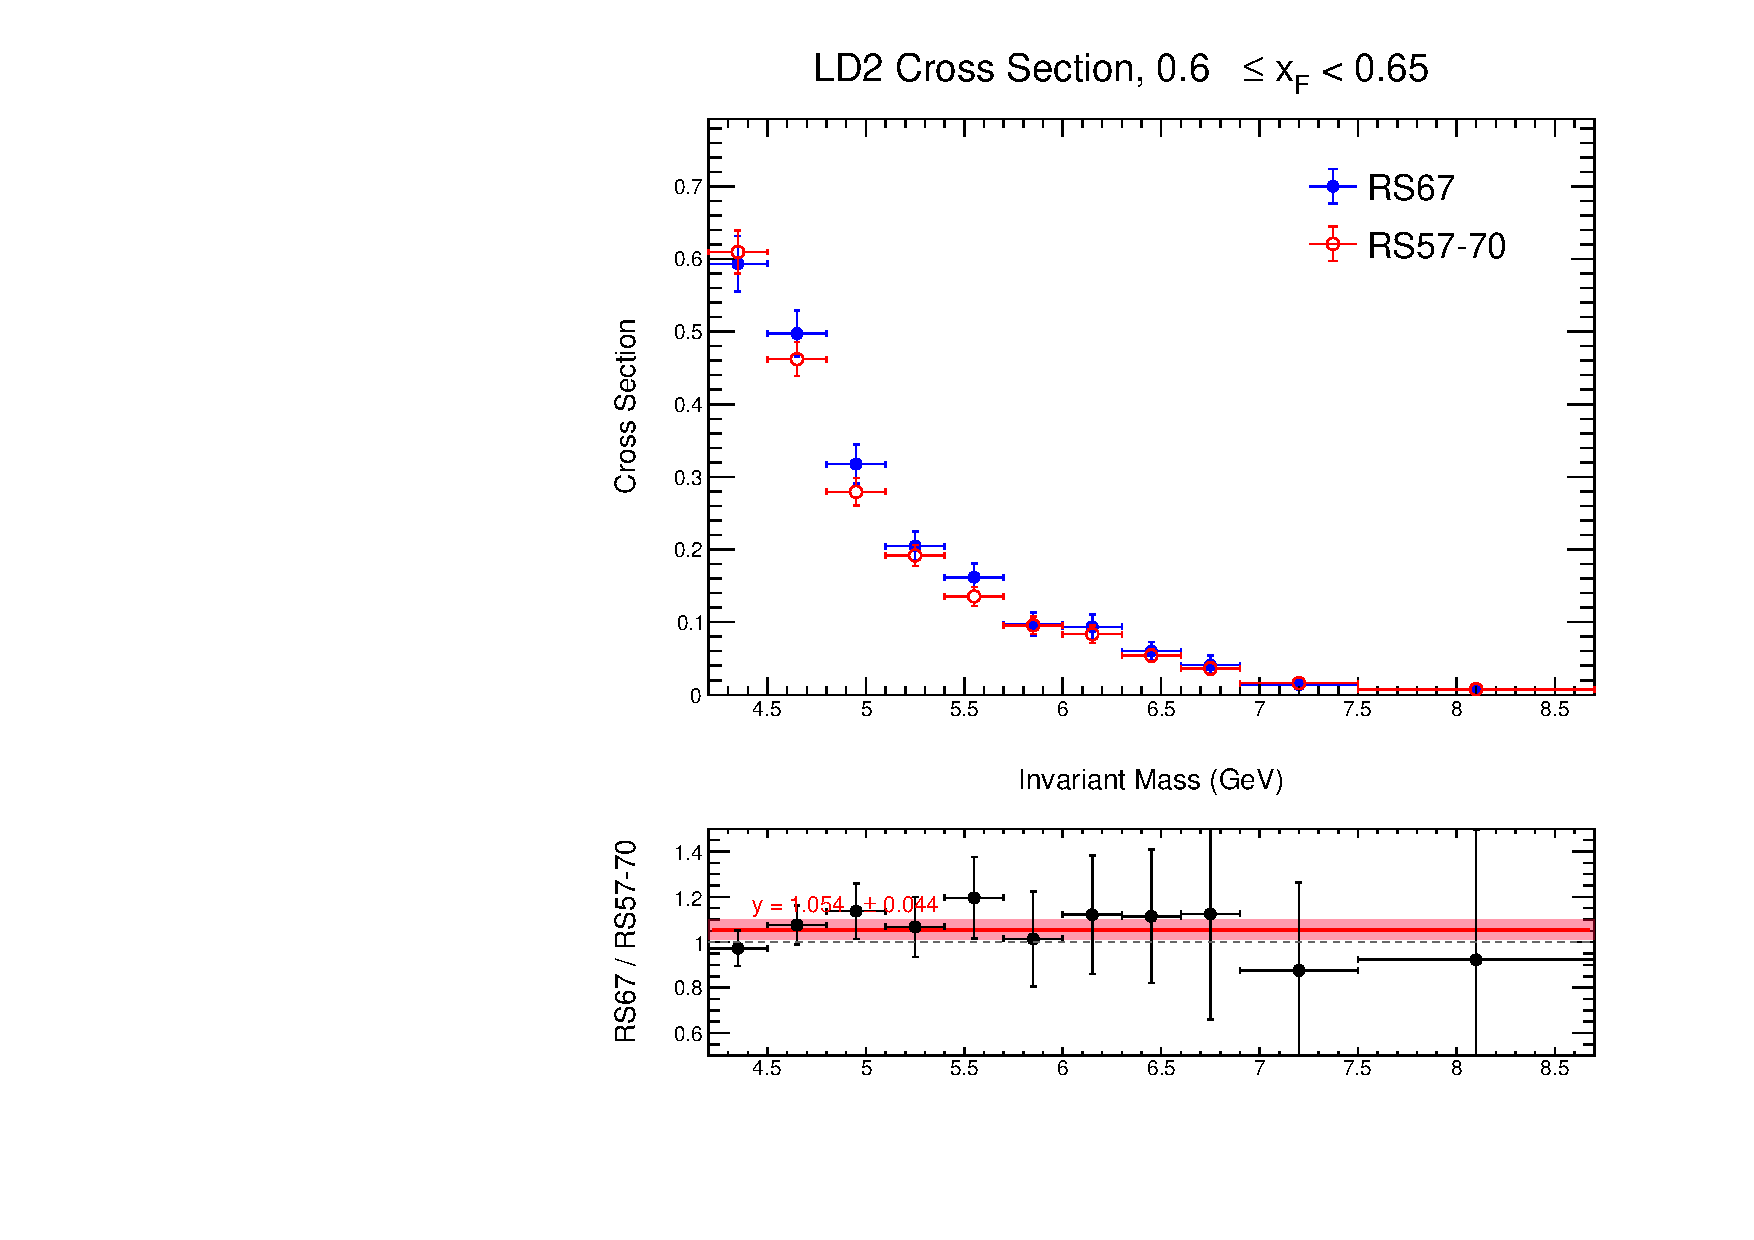
\includegraphics[width=\textwidth]{comparison_plots/XSec_Compare_LD2_xF_12.pdf}
    \end{column}
  \end{columns}
\end{frame}
\begin{frame}{Comparison for $0.65 \leq x_F < 0.7$}
  \begin{columns}
    \begin{column}{0.5\textwidth}
      \centering \textbf{Target: LH2}
      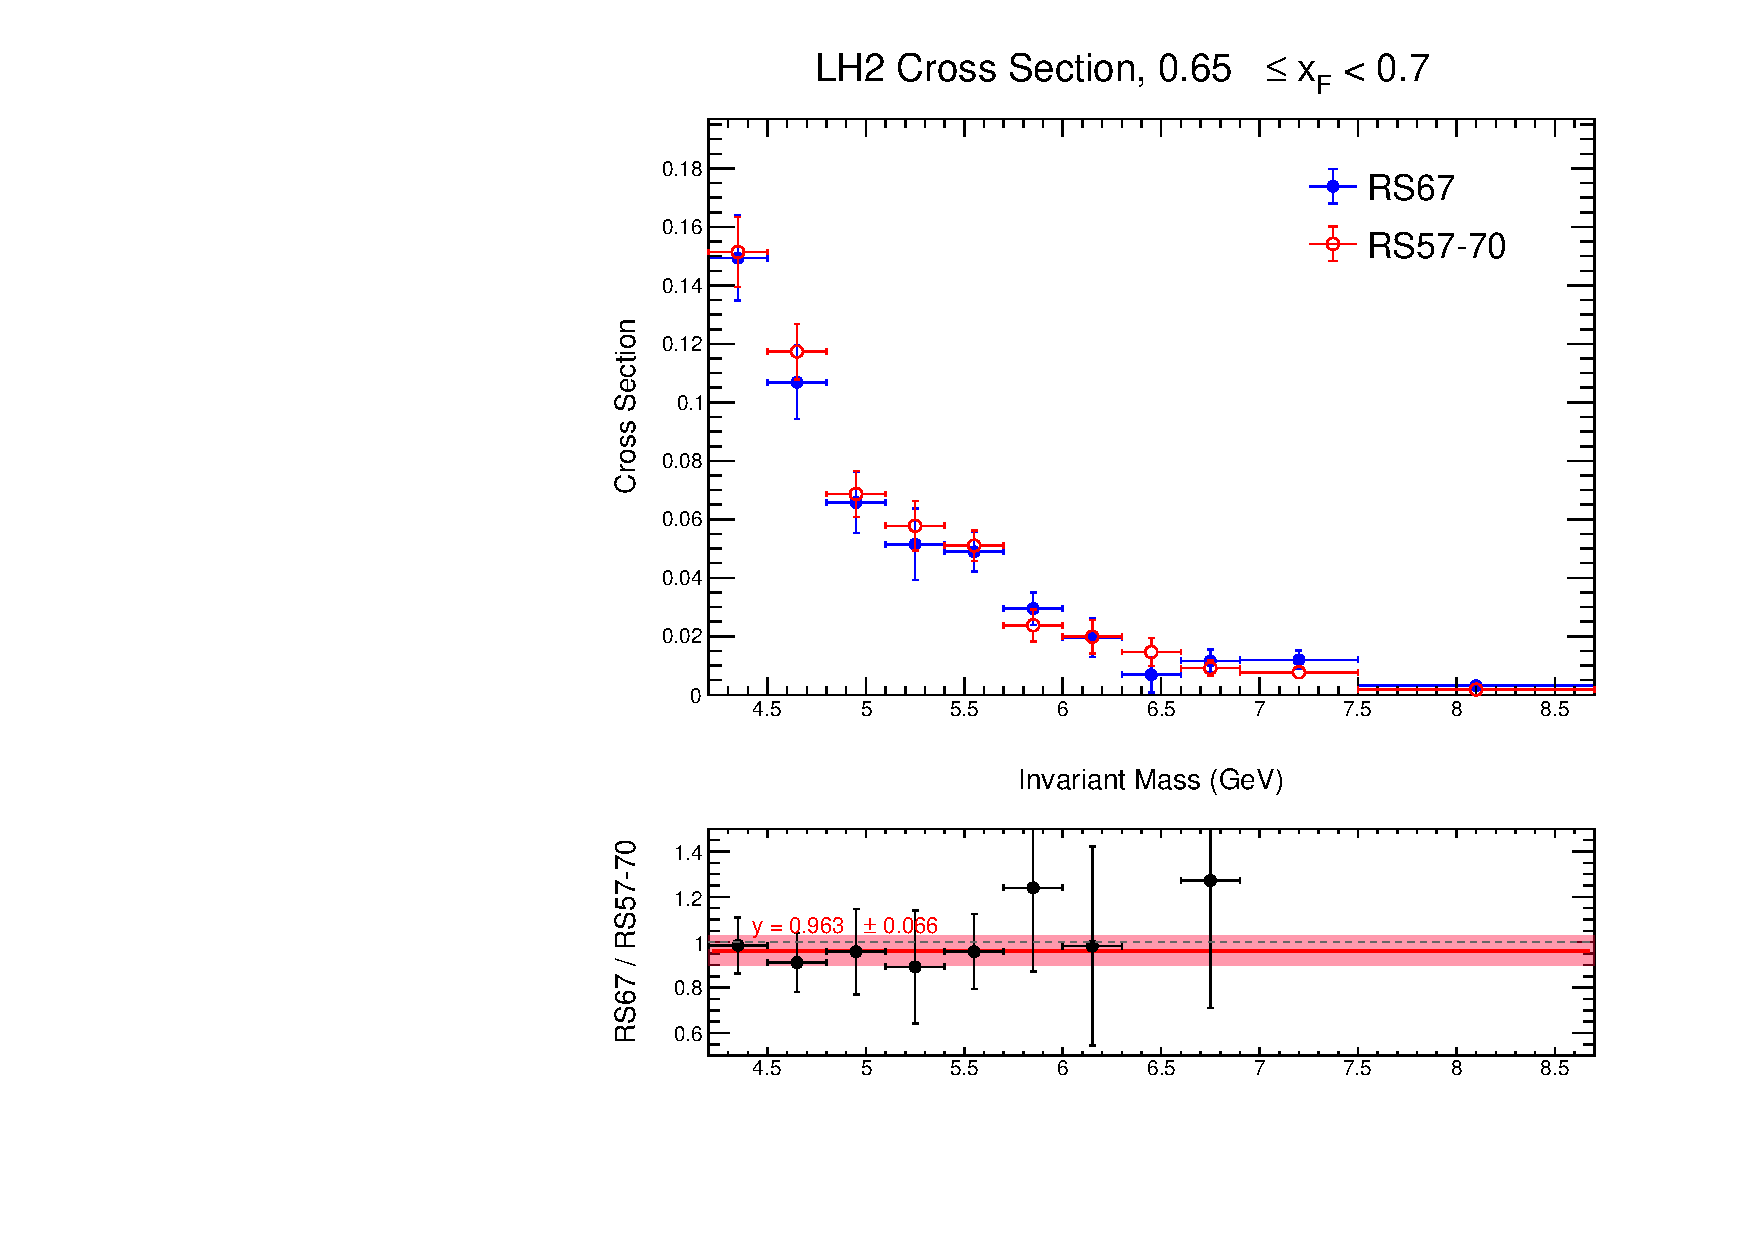
\includegraphics[width=\textwidth]{comparison_plots/XSec_Compare_LH2_xF_13.pdf}
    \end{column}
    \begin{column}{0.5\textwidth}
      \centering \textbf{Target: LD2}
      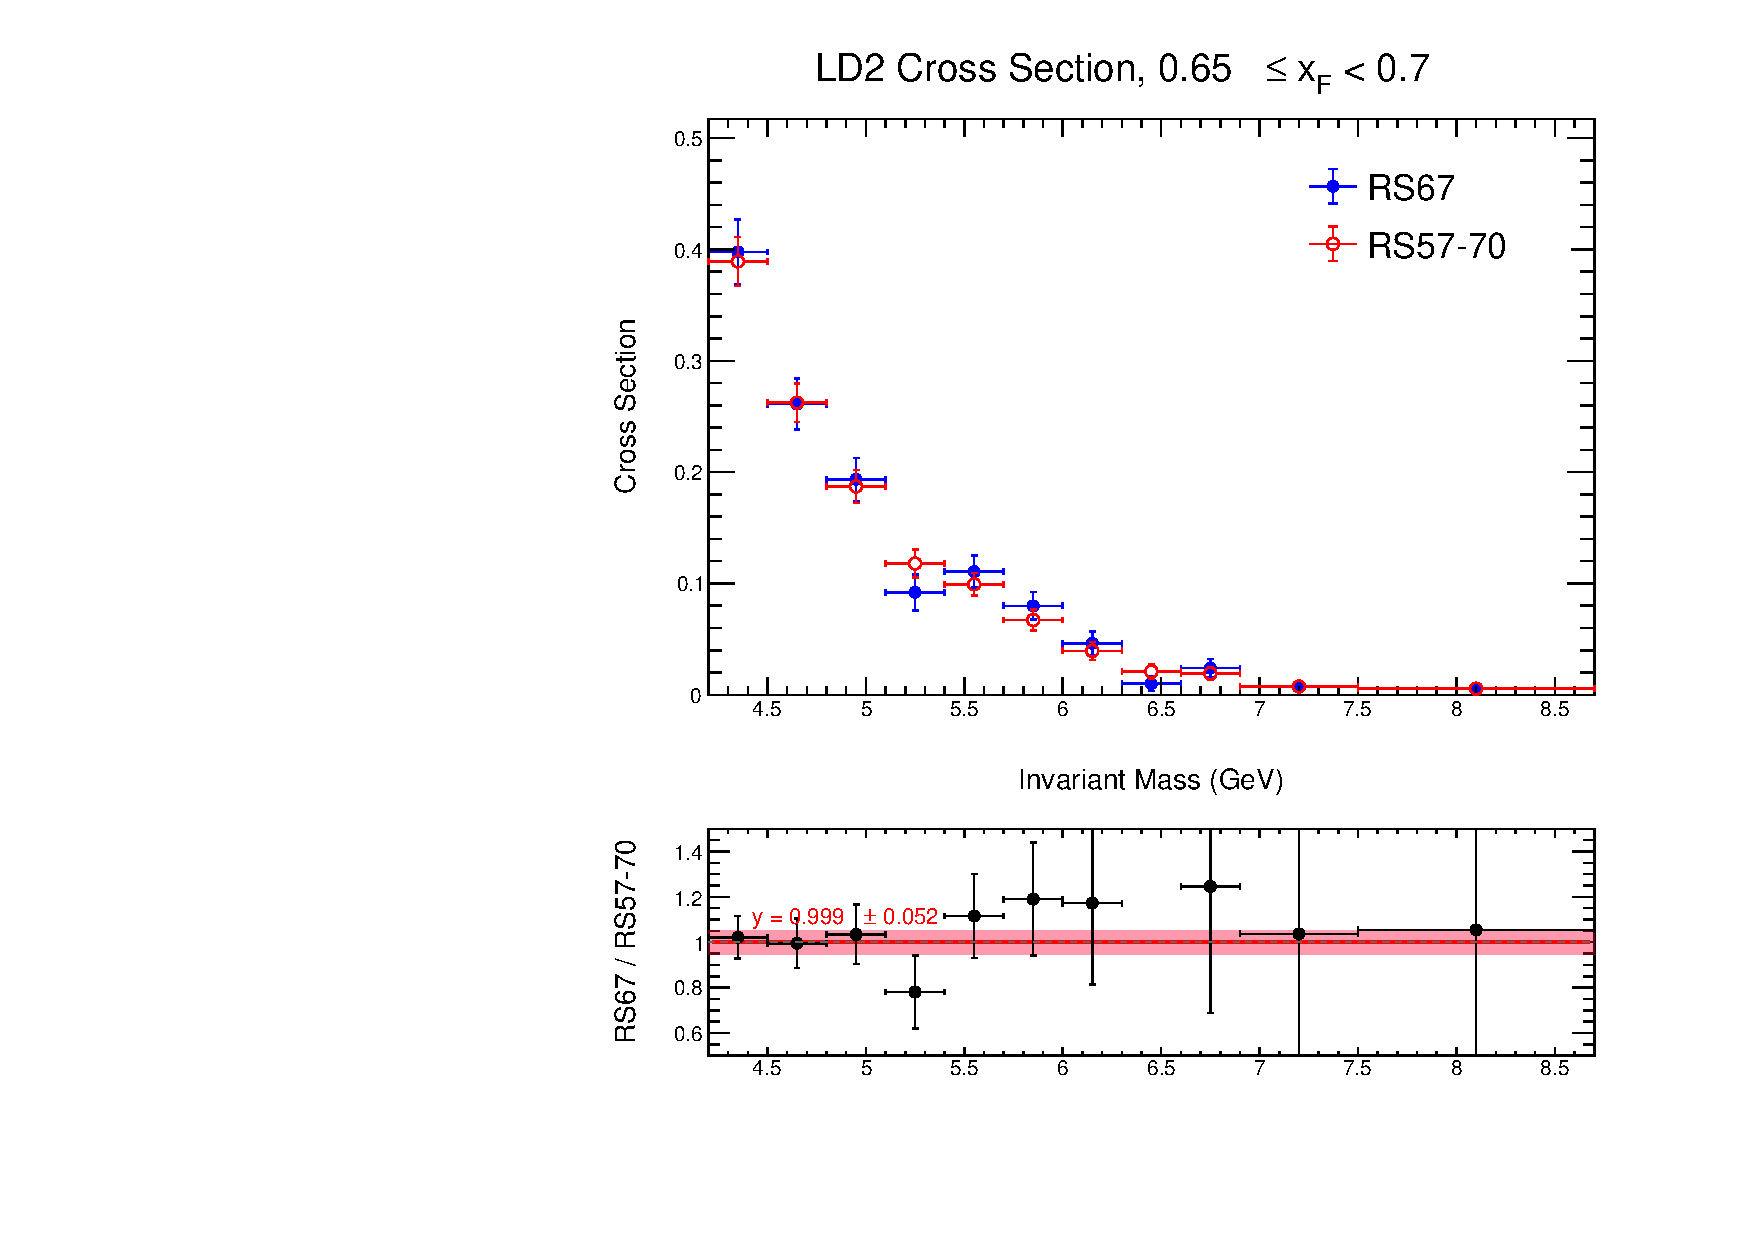
\includegraphics[width=\textwidth]{comparison_plots/XSec_Compare_LD2_xF_13.pdf}
    \end{column}
  \end{columns}
\end{frame}
\begin{frame}{Comparison for $0.7 \leq x_F < 0.75$}
  \begin{columns}
    \begin{column}{0.5\textwidth}
      \centering \textbf{Target: LH2}
      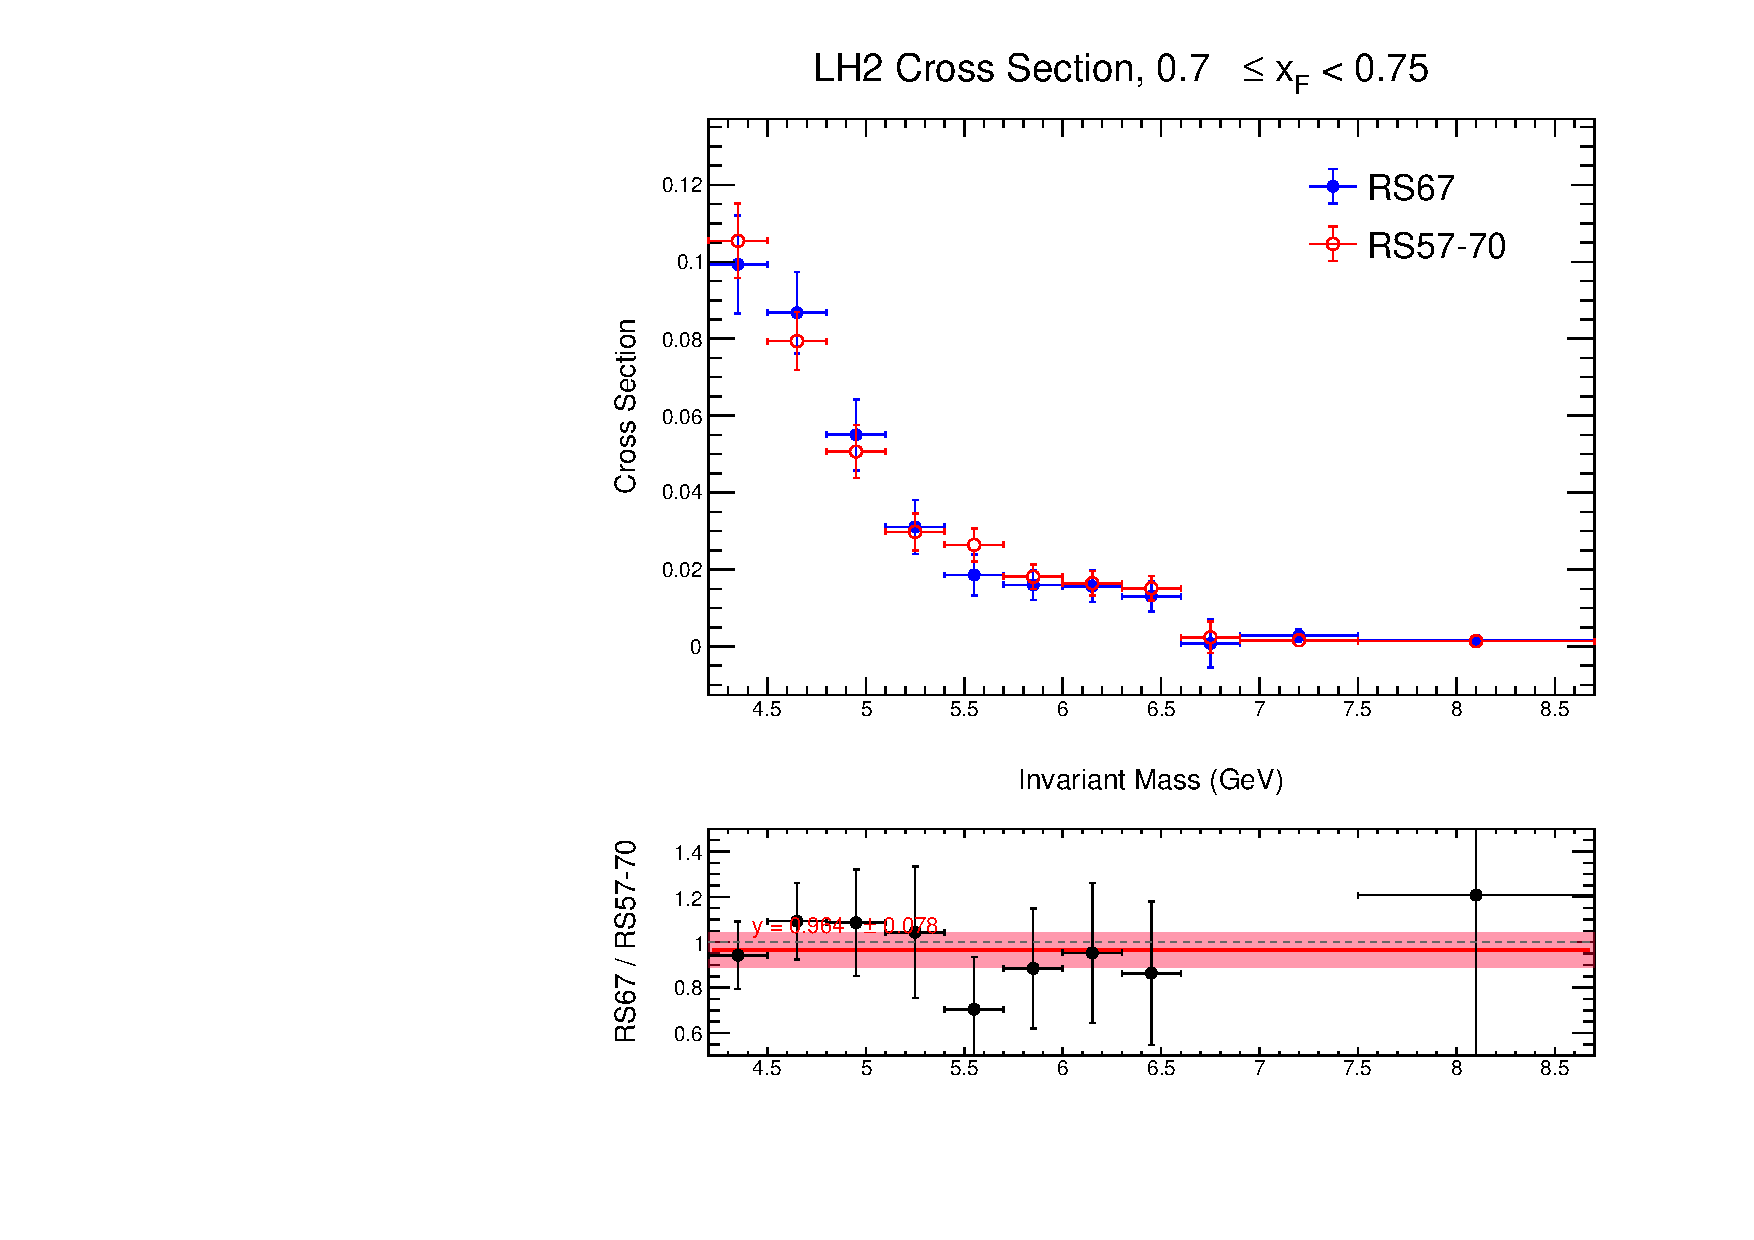
\includegraphics[width=\textwidth]{comparison_plots/XSec_Compare_LH2_xF_14.pdf}
    \end{column}
    \begin{column}{0.5\textwidth}
      \centering \textbf{Target: LD2}
      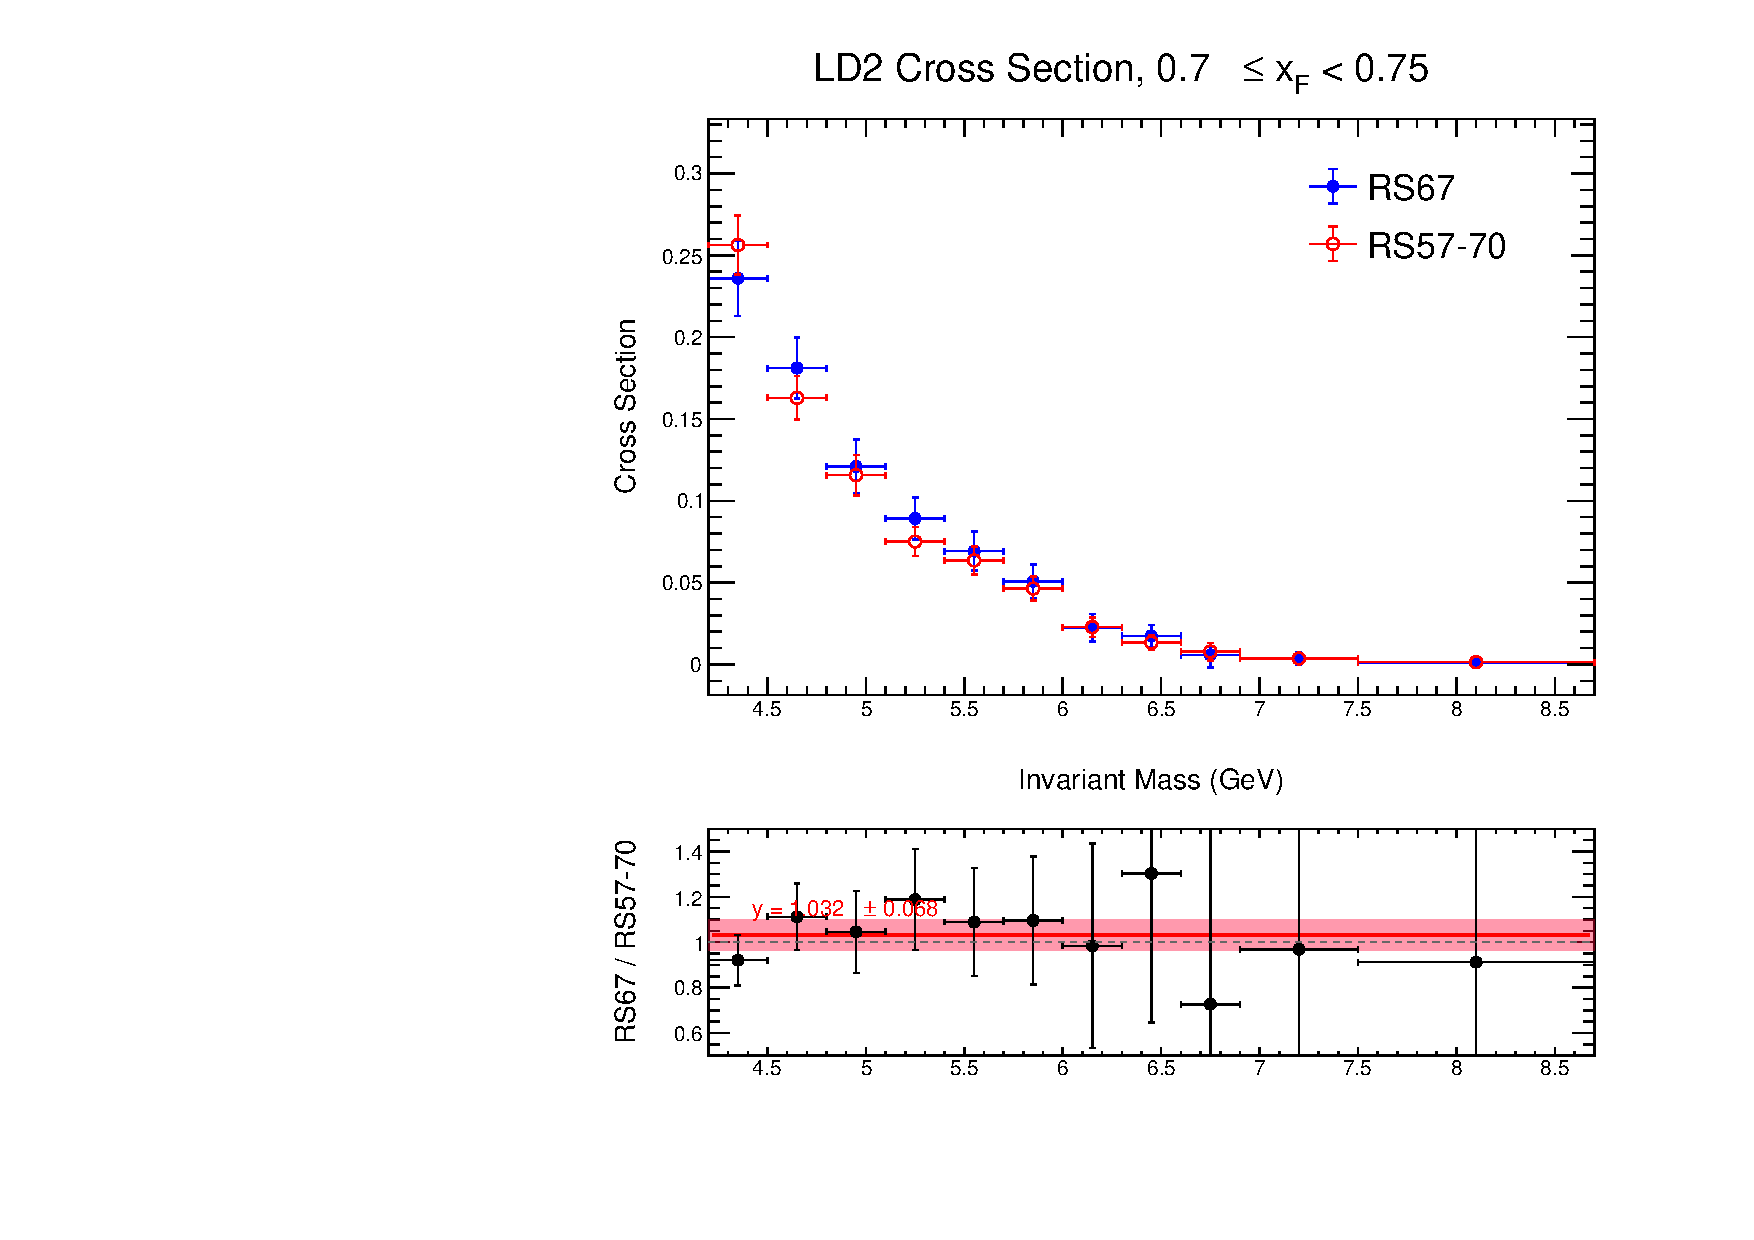
\includegraphics[width=\textwidth]{comparison_plots/XSec_Compare_LD2_xF_14.pdf}
    \end{column}
  \end{columns}
\end{frame}
\begin{frame}{Comparison for $0.75 \leq x_F < 0.8$}
  \begin{columns}
    \begin{column}{0.5\textwidth}
      \centering \textbf{Target: LH2}
      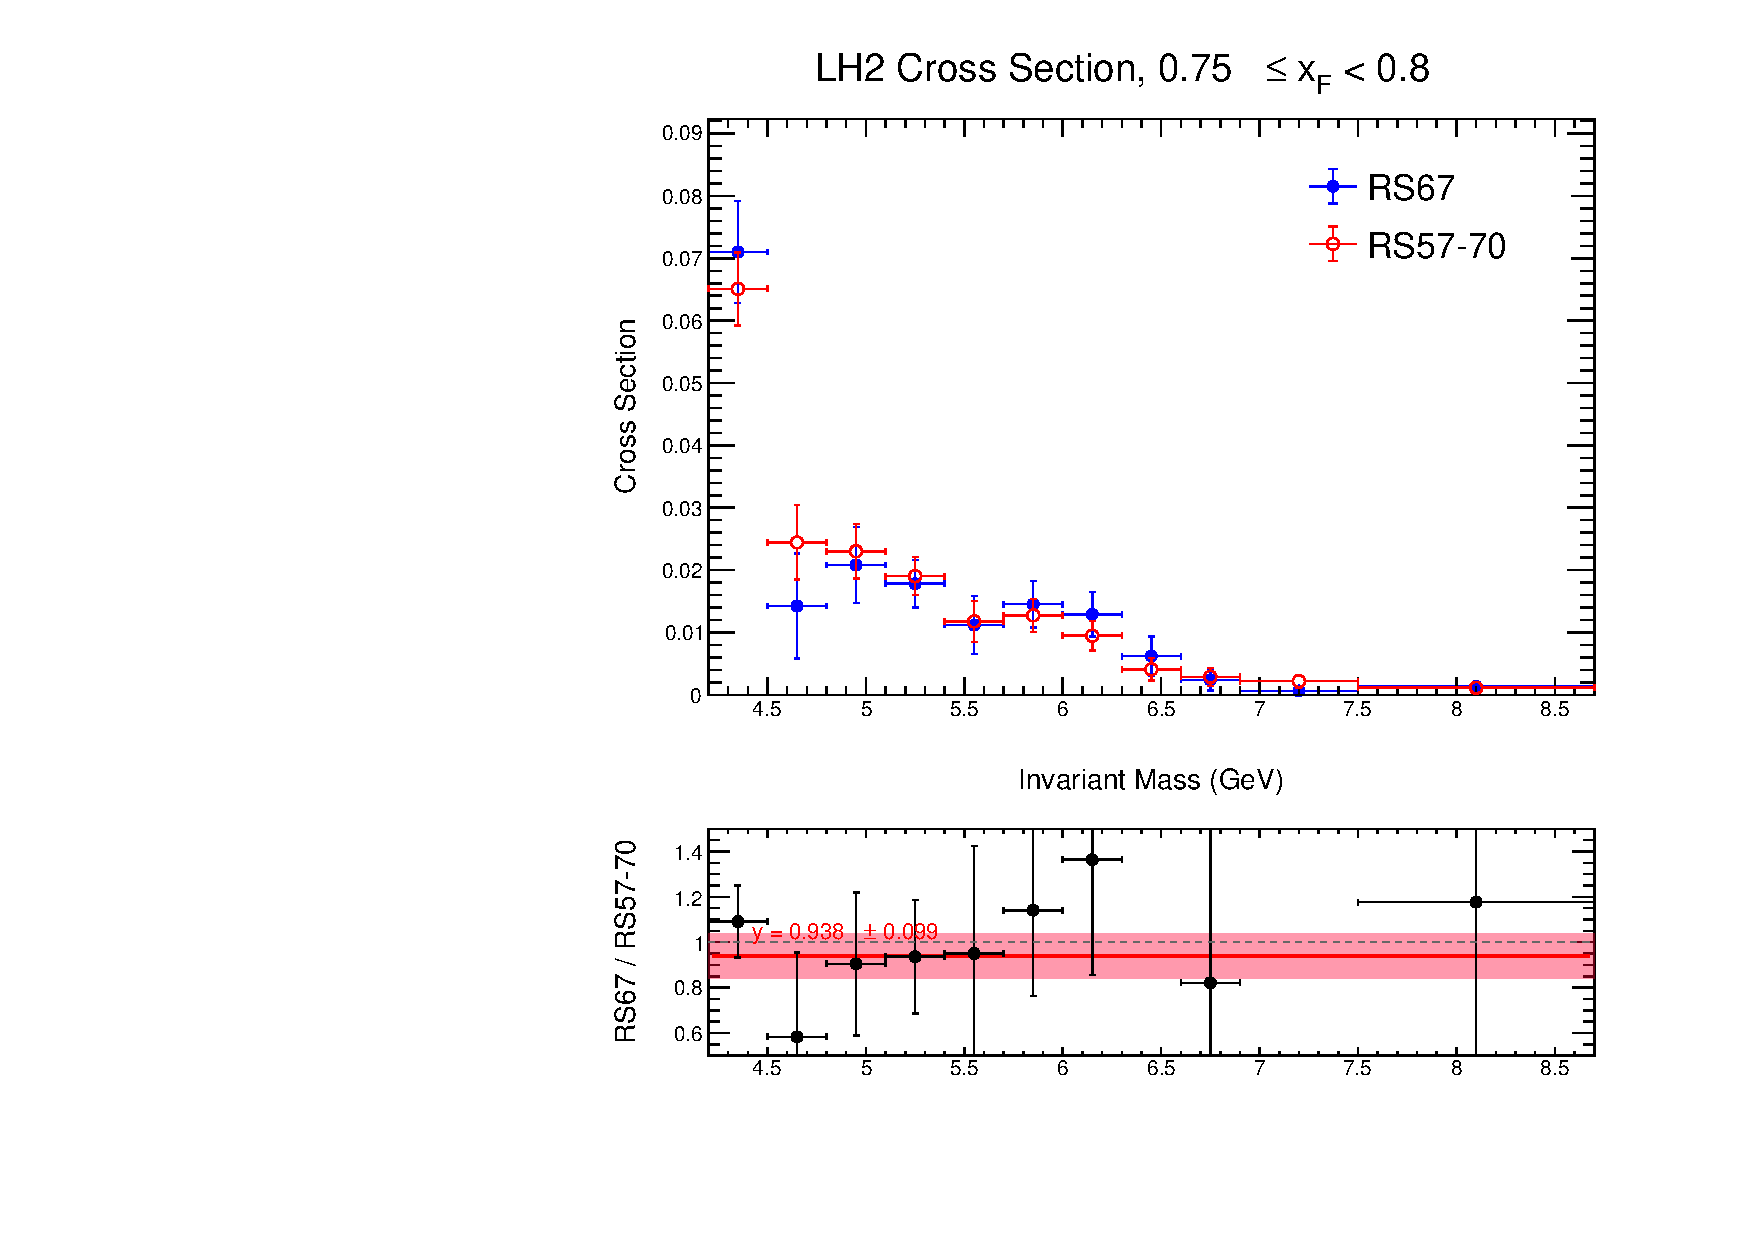
\includegraphics[width=\textwidth]{comparison_plots/XSec_Compare_LH2_xF_15.pdf}
    \end{column}
    \begin{column}{0.5\textwidth}
      \centering \textbf{Target: LD2}
      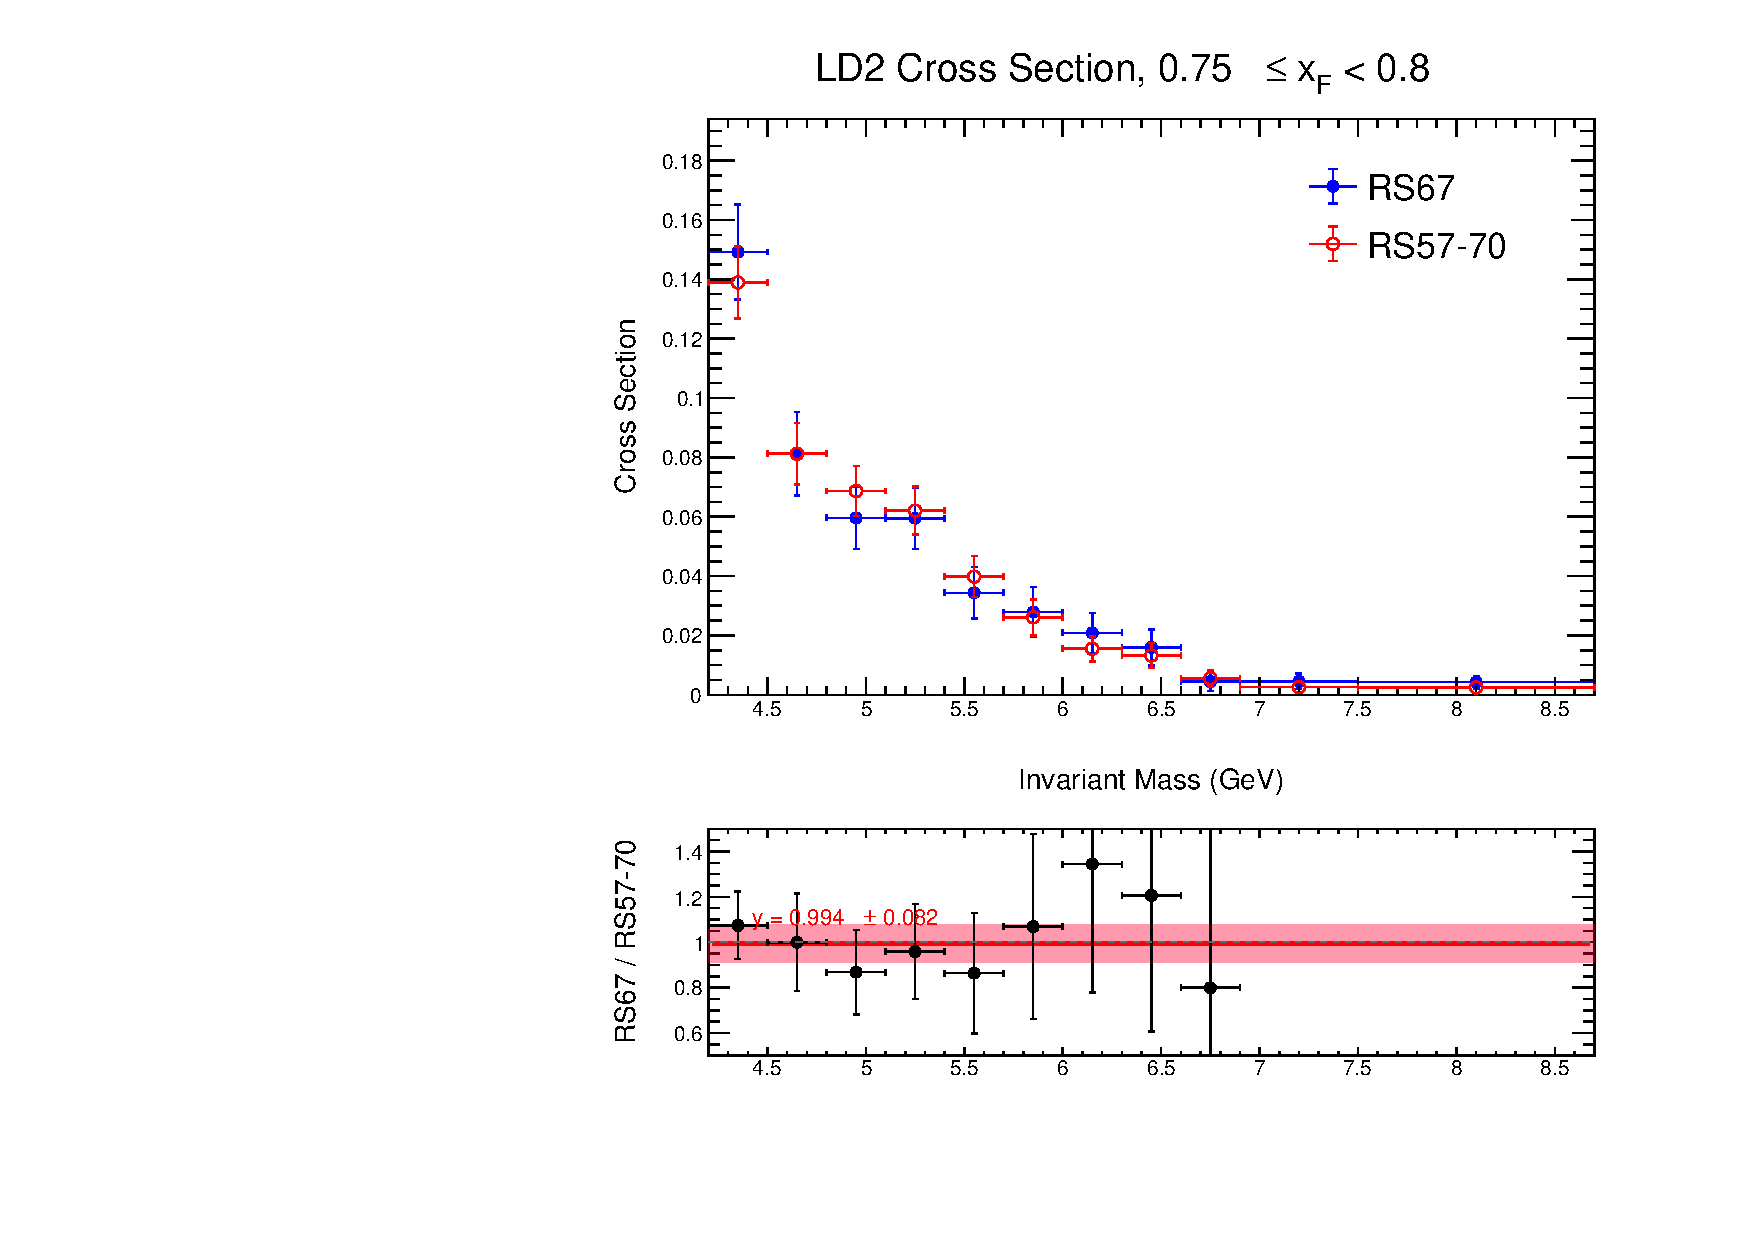
\includegraphics[width=\textwidth]{comparison_plots/XSec_Compare_LD2_xF_15.pdf}
    \end{column}
  \end{columns}
\end{frame}
\end{document}